\chapter{Pedrinhas mágicas}
\markboth{Módulo 1}{}

Neste módulo, vamos trabalhar com os alunos as habilidades
que tratam da manipulação dos algarismos, de modo que o aluno consiga
formar, ordenar e utilizar alguns números, de até 3 ordens, em diversas
aplicações de contagem, ordenação e identificação. 

\colorsec{Habilidades do SAEB}

\begin{itemize}
\item Reconhecer o que os números naturais indicam em diferentes situações:
quantidade, ordem, medida ou código de identificação.
\item Identificar a posição ordinal de um objeto ou termo em uma sequência
(1º, 2º etc.).
\item Escrever números naturais de até 3 ordens em sua representação por
algarismos ou em língua materna ou associar o registro numérico de
números naturais de até 3 ordens ao registro em língua materna.
\item Comparar ou ordenar quantidades de objetos (até 2 ordens).
\item Comparar ou ordenar números naturais de até 3 ordens com ou sem
suporte da reta numérica.
\item Identificar a ordem ocupada por um algarismo ou seu valor posicional
(ou valor relativo) em um número natural de até 3 ordens.
\end{itemize}

\colorsec{Habilidades da BNCC}

\begin{itemize}
\item EF02MA01, EF02MA03.
\end{itemize}
\paragraph{Conteúdo}\label{conteuxfado}

Você já ouviu falar no ábaco? Esse objeto é considerado, por alguns, como
a primeira calculadora do mundo. Existem vários tipos de ábacos. Temos o
chinês, o japonês, o grego, entre outros. Eles servem para representar
números, de várias ordens, além de auxiliar em alguns cálculos de
adição, subtração, multiplicação e até divisão.

\textless{}https://br.freepik.com/vetores-gratis/um-abaco-e-numero-no-quadro-negro\_2956211.htm\#page=2\&query=\%C3\%A1baco\&position=15\&from\_view=search\&track=sph.
Favor trocar a vírgula do número por um ponto, ou por um espaço
vazio.\textgreater{}

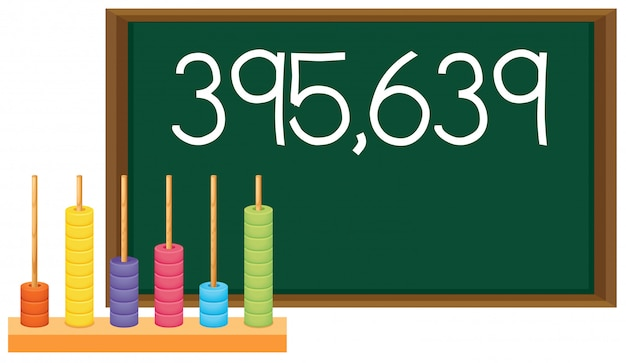
\includegraphics[width=3.51042in,height=2.03550in]{media/image1.jpeg}

O ábaco da figura é o mais simples e serve somente para representar
números de até 6 ordens. Perceba que cada ordem contém a quantidade de
pedrinhas correspondente ao algarismo que a representa. A primeira haste, da direita, tem 9 pedrinhas verdes, representando o algarismo
nove, da ordem das unidades. A haste logo à esquerda representa a
ordem das dezenas e assim por diante.

\textless{}https://br.freepik.com/fotos-gratis/garotinho-tendo-uma-sessao-de-terapia-ocupacional\_18036725.htm\#query=\%C3\%A1baco\%20japon\%C3\%AAs\&position=45\&from\_view=search\&track=ais\textgreater{}

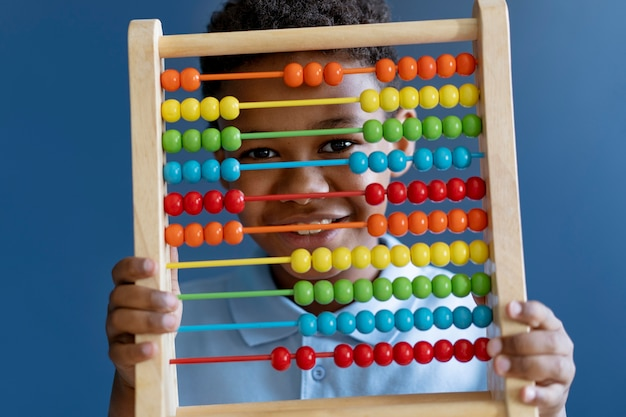
\includegraphics[width=4.73800in,height=3.15625in]{media/image2.jpeg}

Nessa figura temos um ábaco mais conhecido, onde hastes
horizontais representam as ordens dos números. Para representar o
número zero, posicionamos todas as bolinhas do lado esquerdo. Se
puxarmos duas bolinhas da primeira haste de baixo para a direita, mais
três bolinhas da próxima haste também para a direita, formamos o número
32. Nesse ábaco é possível realizar operações simples, sobrepondo as
pedrinhas que queremos adicionar, por exemplo.

Se possível, leve um ábaco para a sala de aula e demonstre
alguns números aos alunos; ou, então, permita que eles façam alguns.

\paragraph{Atividades }\label{atividades}

\subparagraph{1.}\label{section}

Ligue os números das figuras a seguir, de acordo com o que esses números
representam.

\textless{}https://br.freepik.com/vetores-gratis/ilustracao-de-barcode\_3232987.htm\#query=codigo\%20de\%20barras\&position=2\&from\_view=search\&track=ais;
https://br.freepik.com/fotos-premium/nota-de-cem-reais-do-brasil-caindo-sobre-fundo-branco-isolado\_27213030.htm\#query=dinheiro\&position=10\&from\_view=search\&track=sph;
https://br.freepik.com/vetores-gratis/podio-do-vencedor-de-esportes-iluminados_1529256.htm#query=podium&position=36&from_view=search&track=sph

\begin{longtable}[]{@{}ll@{}}
\toprule
\begin{minipage}[b]{0.48\columnwidth}\raggedright\strut
CÓDIGO DE

IDENTIFICAÇÃO\strut
\end{minipage} & \begin{minipage}[b]{0.48\columnwidth}\raggedright\strut
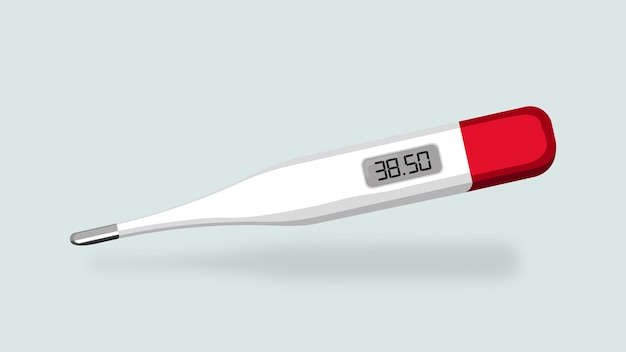
\includegraphics[width=2.28891in,height=0.67601in]{media/image3.jpeg}\strut
\end{minipage}\tabularnewline
\midrule
\endhead
QUANTIDADE &
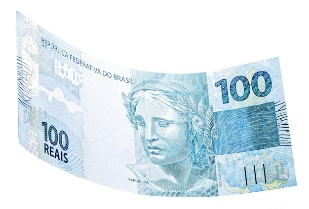
\includegraphics[width=1.39514in,height=0.94497in]{media/image4.jpeg}\tabularnewline
ORDEM &

\includegraphics[width=1.19792in,height=0.69792in]{media/image5.jpeg}\tabularnewline
MEDIDA &
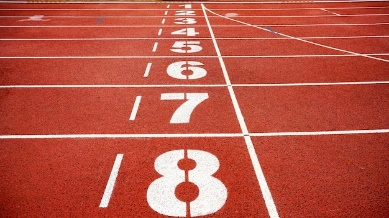
\includegraphics[width=1.75972in,height=0.98664in]{media/image6.jpeg}\tabularnewline
\bottomrule
\end{longtable}

Oriente os alunos a pensarem na função que cada número
exerce, nas aplicações em que são apresentados, antes de escolherem a
relação.

\subparagraph{2. }\label{section-1}

Pinte o quadrado que contém o 5° número da sequência de números a seguir.
Cuidado! Esses números estão fora da ordem; portanto, você deve
ordená-los primeiro.

\begin{longtable}[]{@{}llllllllll@{}}
\toprule
56 & 32 & 78 & 21 & 47 & 14 & 03 & 97 & 10 & 28\tabularnewline
\bottomrule
\end{longtable}

Oriente os alunos a primeiramente ordenar os números em
uma folha separada. Algum aluno pode, afoitamente, pintar o quinto
quadradinho.

\subparagraph{3. }\label{section-2}

Escreva por extenso os números representados nos ábacos. A ordem
é crescente da direita para a esquerda, ou seja, a primeira haste da
direita representa as unidades e assim por diante.

\textless{}Inserir as figuras de ábacos, conforme as imagens a
seguir. Colocar quadros ao lado das figuras com a indicação de
linhas.\textgreater{}

\begin{longtable}[]{@{}ll@{}}
\toprule
\begin{minipage}[b]{0.48\columnwidth}\raggedright\strut
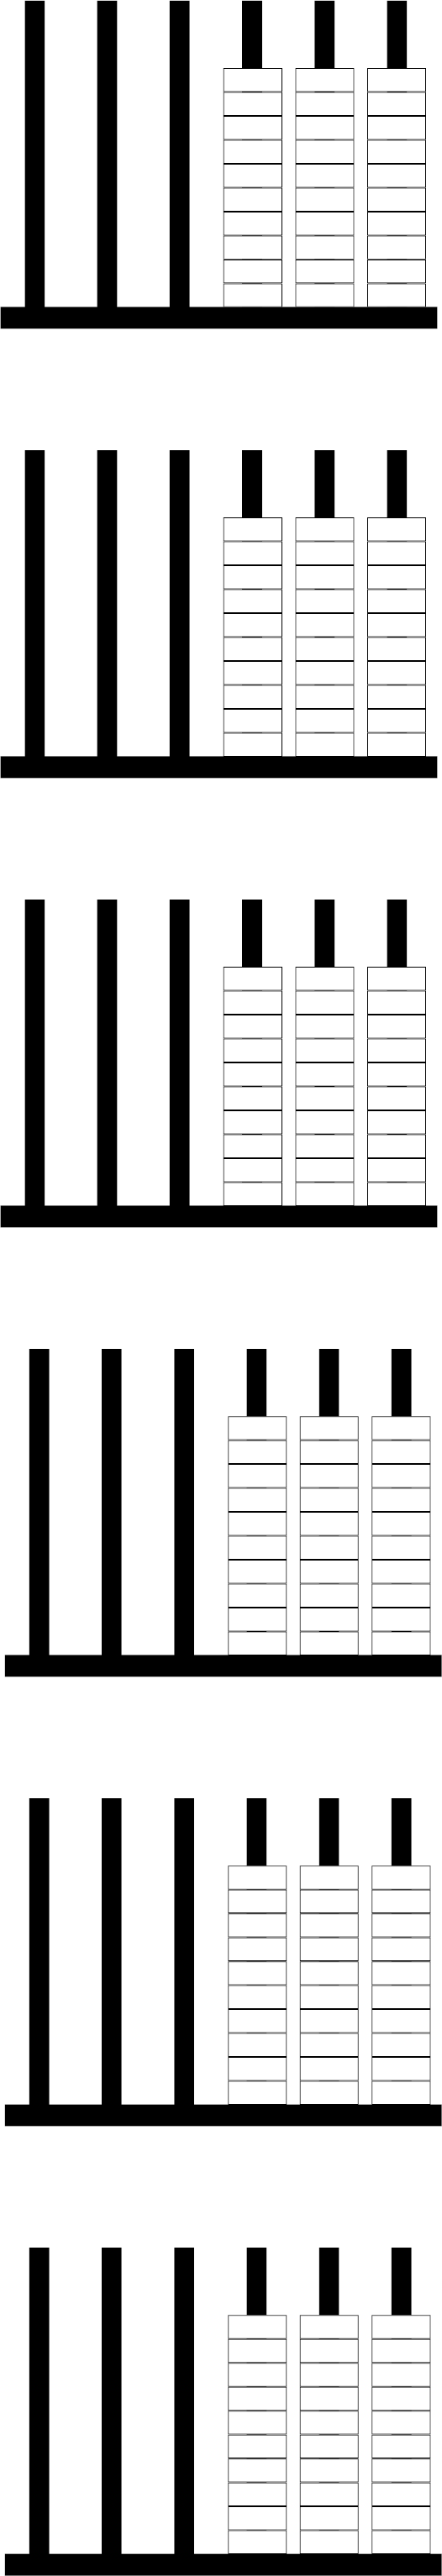
\includegraphics[width=2.46062in,height=1.44792in]{media/image7.png}\strut
\end{minipage} & \begin{minipage}[b]{0.48\columnwidth}\raggedright\strut
\textless{}4 linhas\textgreater{}

Oitocentos e trinta e quatro.\strut
\end{minipage}\tabularnewline
\midrule
\endhead
\begin{minipage}[t]{0.48\columnwidth}\raggedright\strut
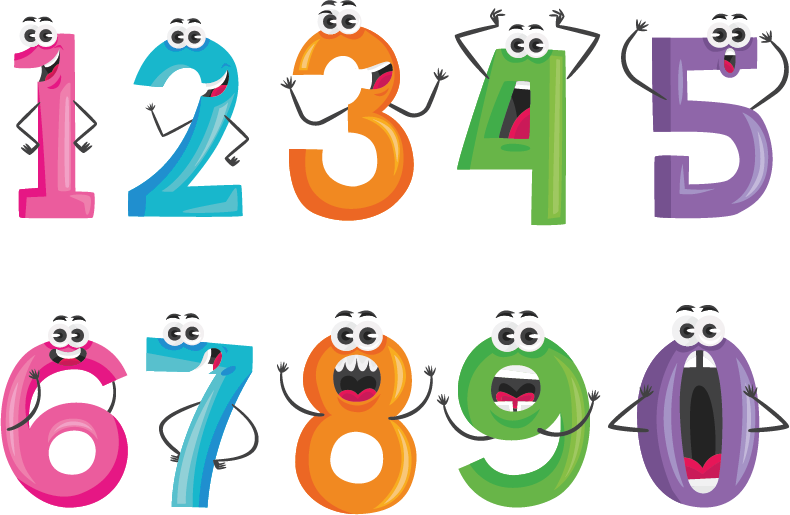
\includegraphics[width=2.40625in,height=1.57296in]{media/image8.png}\strut
\end{minipage} & \begin{minipage}[t]{0.48\columnwidth}\raggedright\strut
\textless{}4 linhas\textgreater{}

Quinhentos e trinta e nove.\strut
\end{minipage}\tabularnewline
\begin{minipage}[t]{0.48\columnwidth}\raggedright\strut
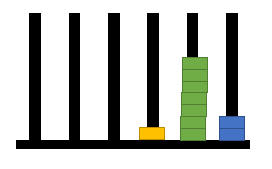
\includegraphics[width=2.45833in,height=1.52742in]{media/image9.png}\strut
\end{minipage} & \begin{minipage}[t]{0.48\columnwidth}\raggedright\strut
\textless{}4 linhas\textgreater{}

Cento e setenta e dois.\strut
\end{minipage}\tabularnewline
\begin{minipage}[t]{0.48\columnwidth}\raggedright\strut
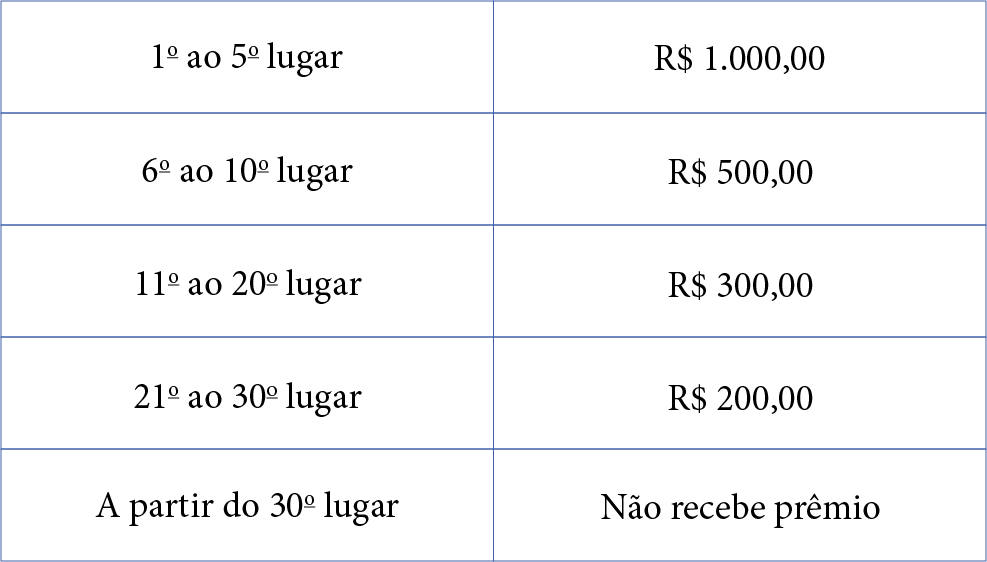
\includegraphics[width=2.40625in,height=1.53287in]{media/image10.png}\strut
\end{minipage} & \begin{minipage}[t]{0.48\columnwidth}\raggedright\strut
\textless{}4 linhas\textgreater{}

Cento e onze.\strut
\end{minipage}\tabularnewline
\begin{minipage}[t]{0.48\columnwidth}\raggedright\strut
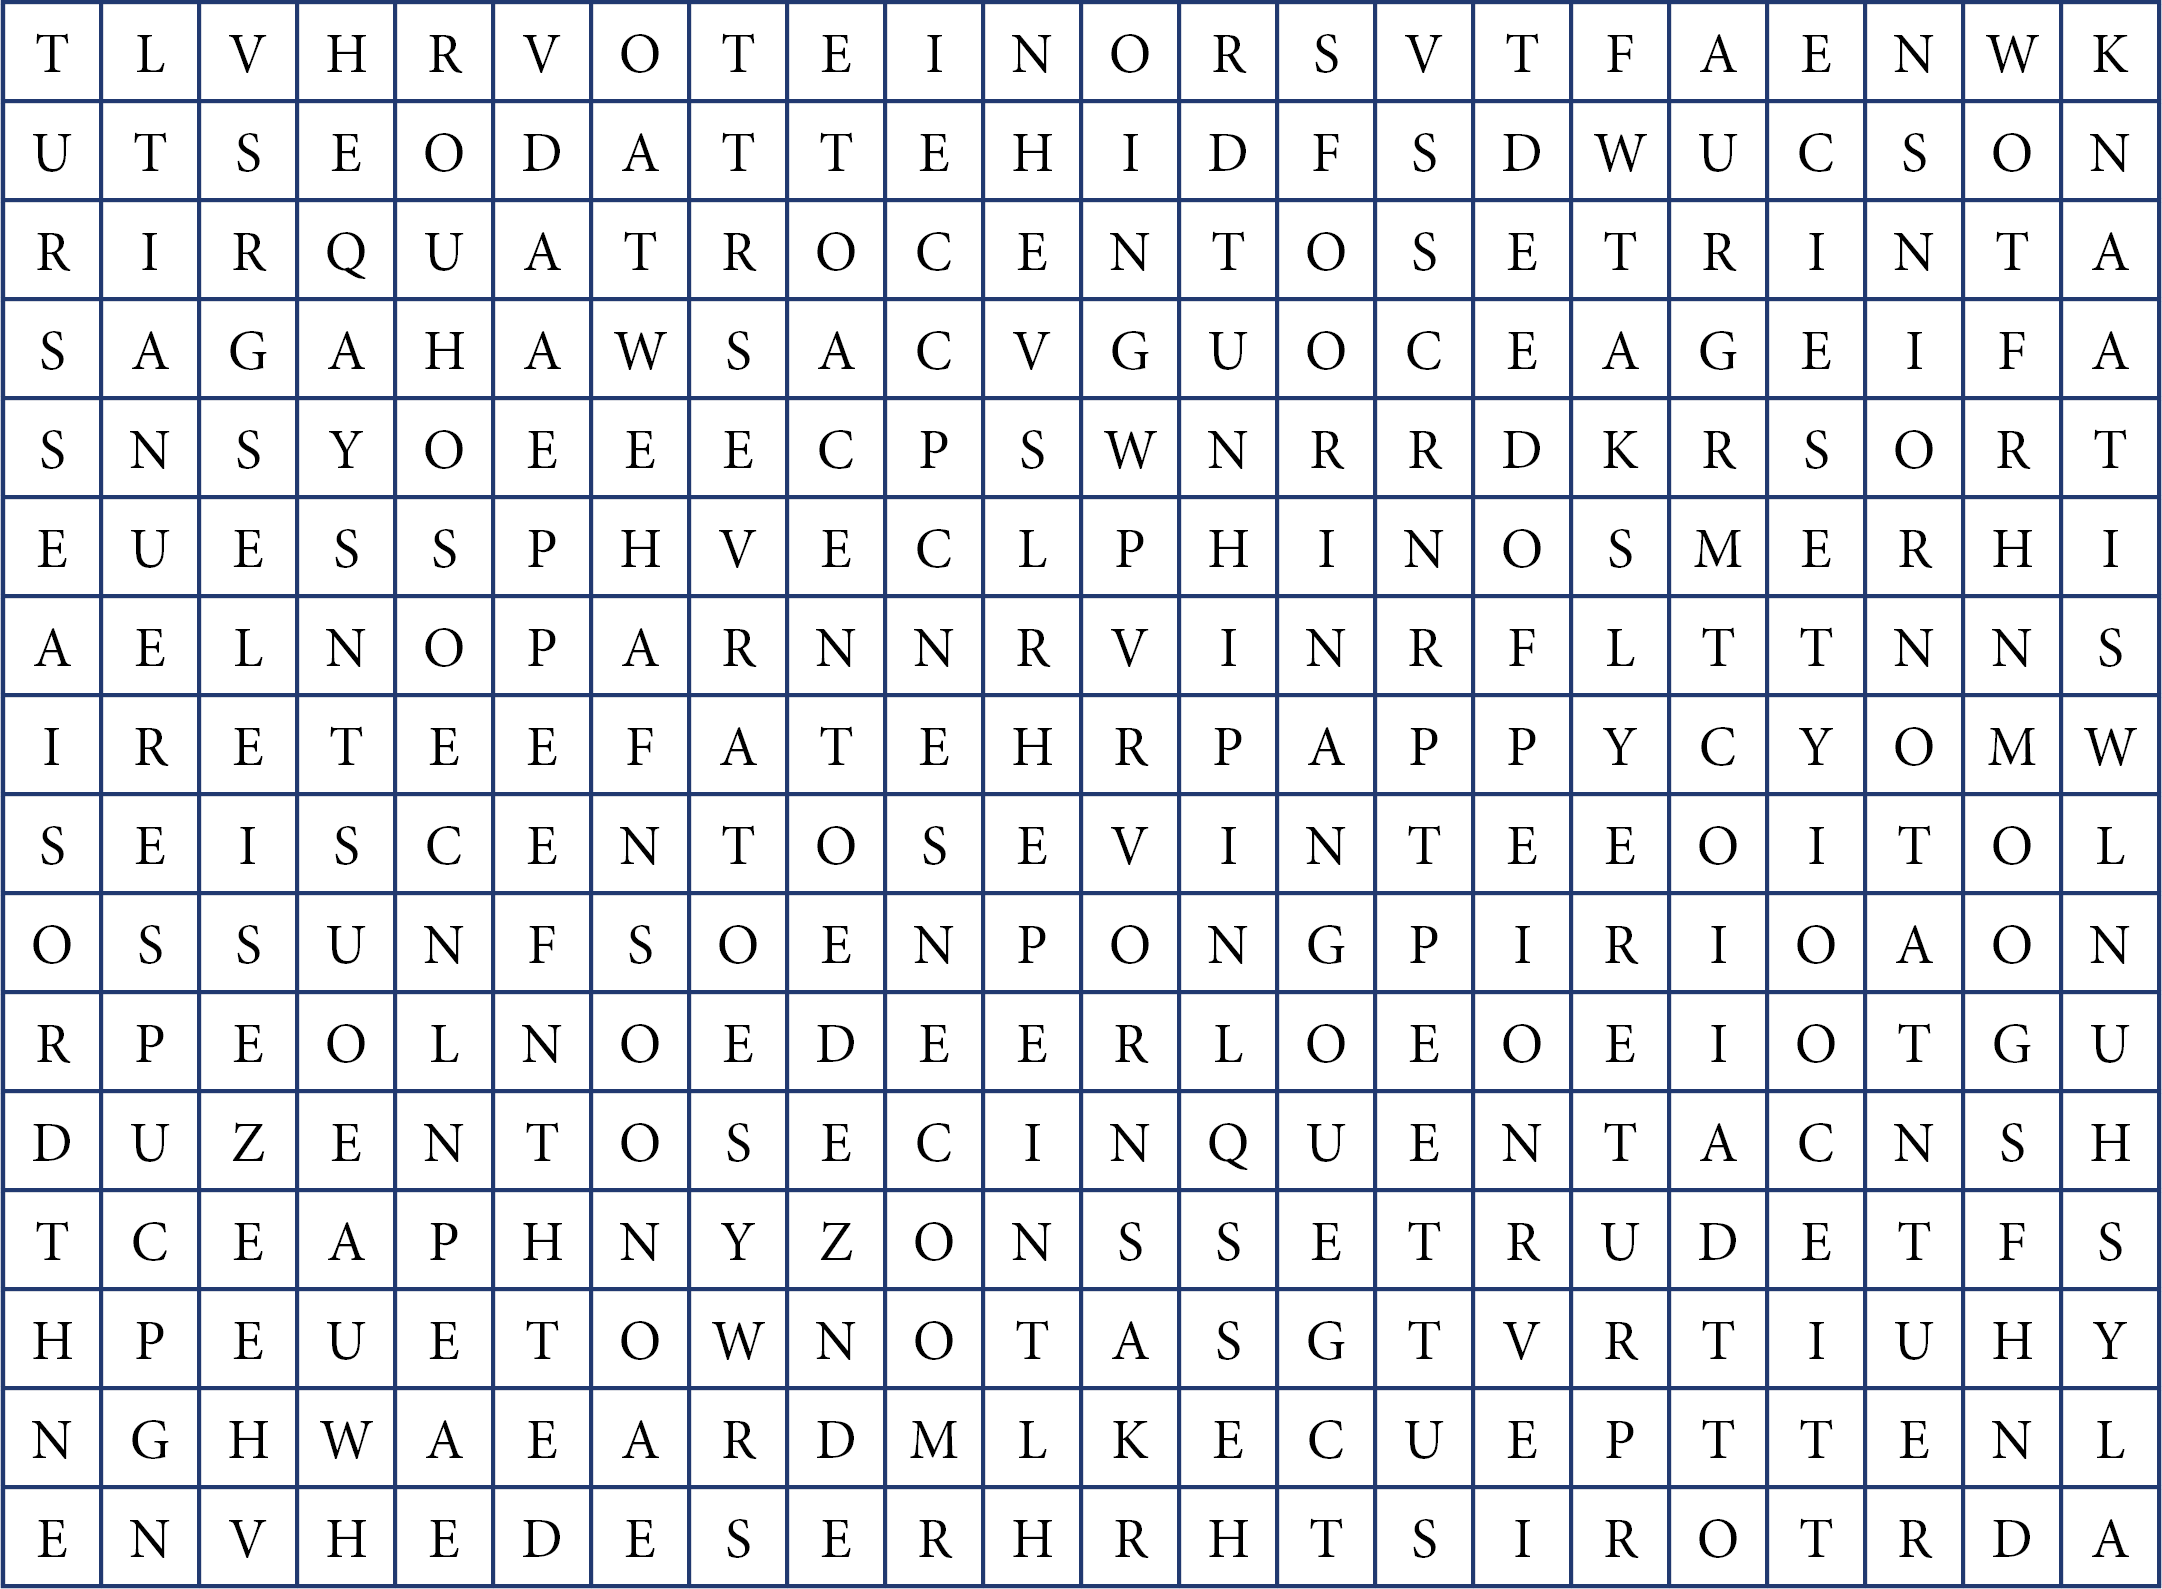
\includegraphics[width=2.45833in,height=1.55359in]{media/image11.png}\strut
\end{minipage} & \begin{minipage}[t]{0.48\columnwidth}\raggedright\strut
\textless{}4 linhas\textgreater{}

Novecentos e noventa e nove.\strut
\end{minipage}\tabularnewline
\begin{minipage}[t]{0.48\columnwidth}\raggedright\strut
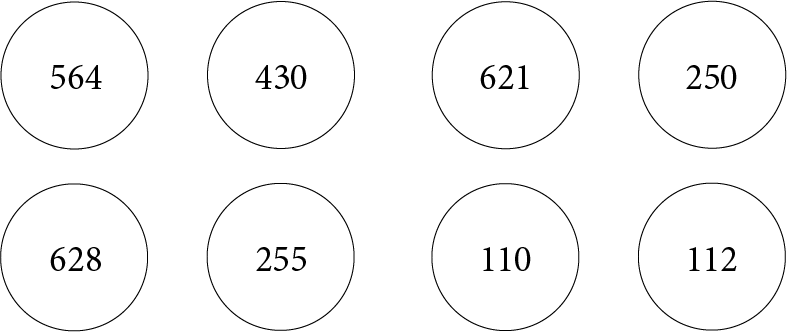
\includegraphics[width=2.40625in,height=1.40287in]{media/image12.png}\strut
\end{minipage} & \begin{minipage}[t]{0.48\columnwidth}\raggedright\strut
\textless{}4 linhas\textgreater{}

Seiscentos e cinquenta e oito.\strut
\end{minipage}\tabularnewline
\bottomrule
\end{longtable}

Oriente os alunos a não escreverem os algarismos, mas sim
a escreverem os números por extenso, em língua portuguesa.

\subparagraph{4. }\label{section-3}

Ordene os números representados nos ábacos, preenchendo os
números nos quadros abaixo das letras. Depois, ordene as letras no
quadro das posições.

\textless{}Inserir a figura dos ábacos, conforme os modelos
abaixo\textgreater{}

\begin{longtable}[]{@{}llll@{}}
\toprule
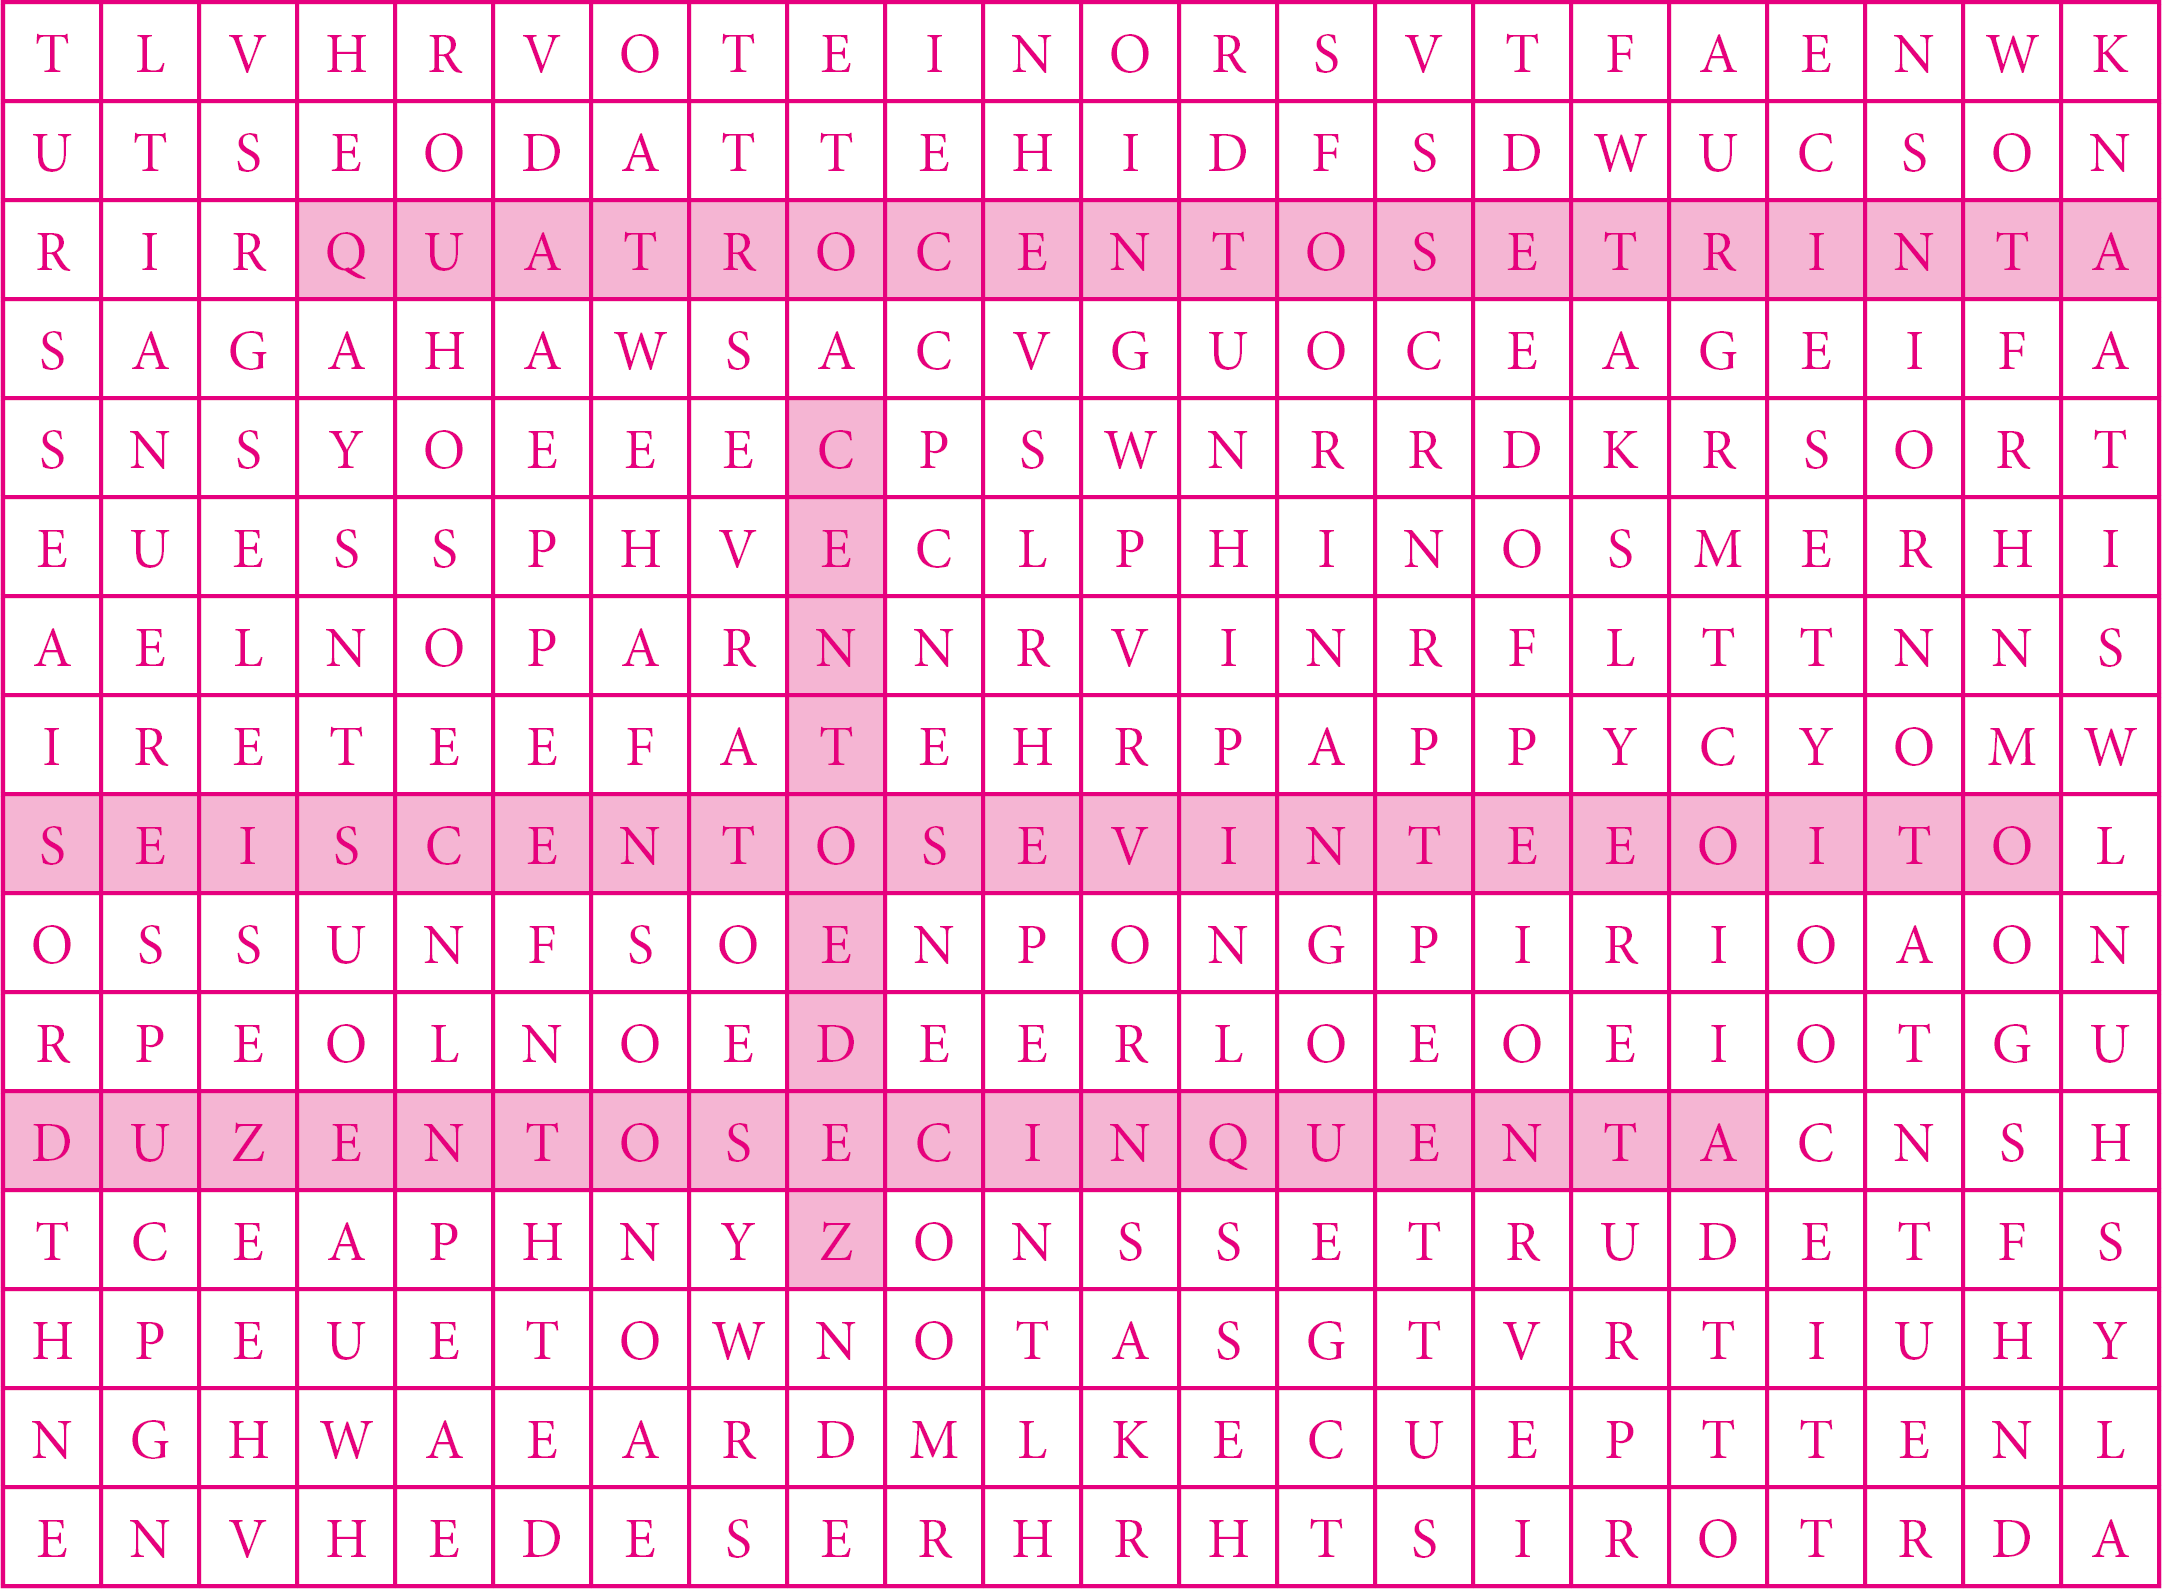
\includegraphics[width=1.24938in,height=0.76667in]{media/image13.png} &
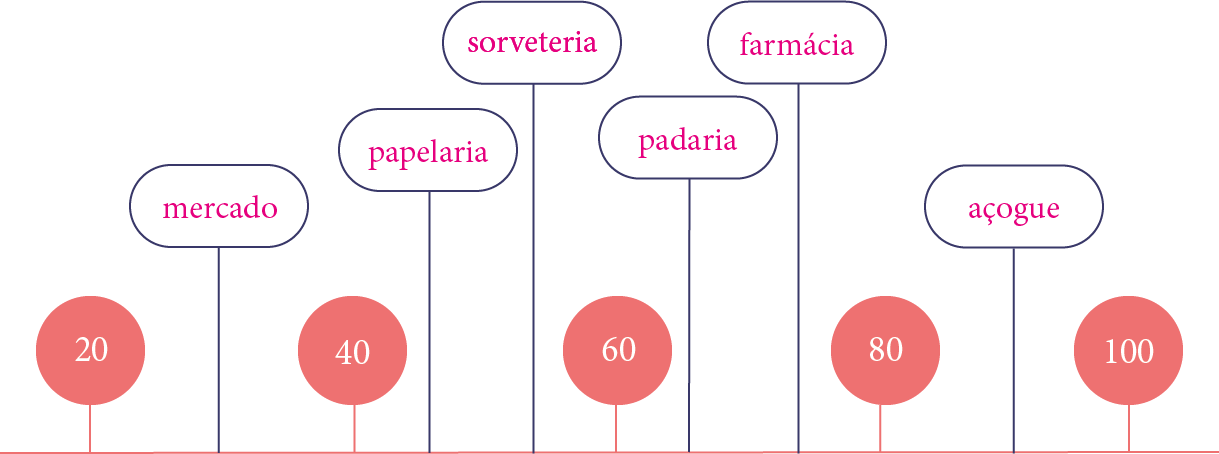
\includegraphics[width=1.35417in,height=0.78502in]{media/image14.png} &
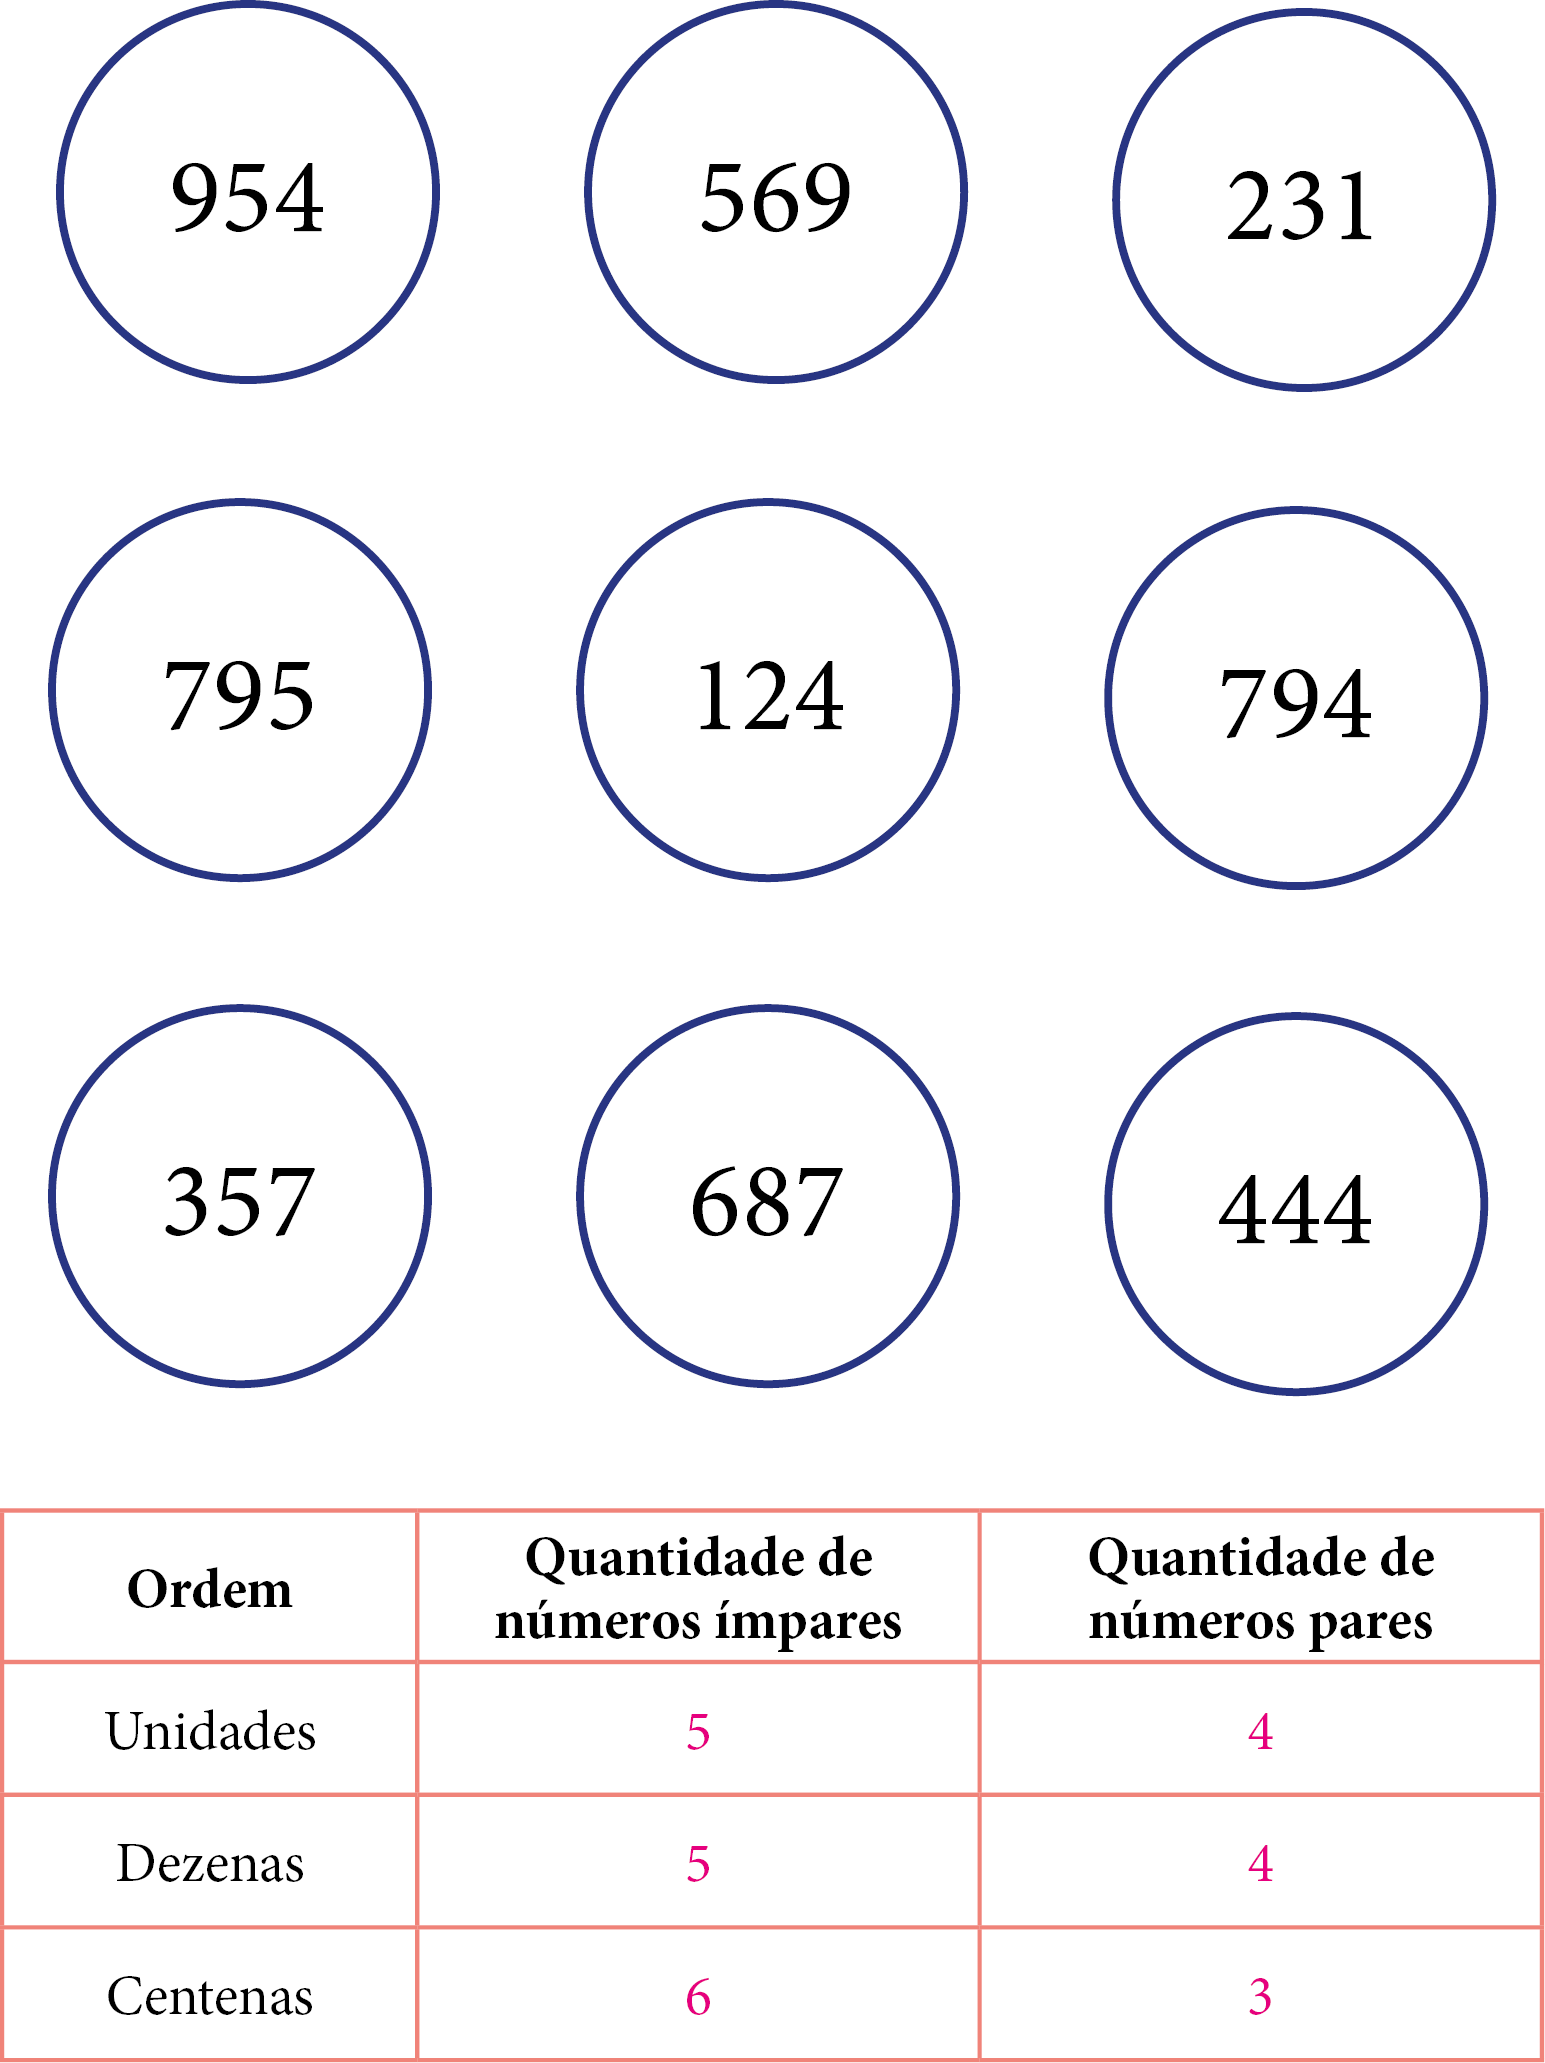
\includegraphics[width=1.29167in,height=0.76677in]{media/image15.png} &
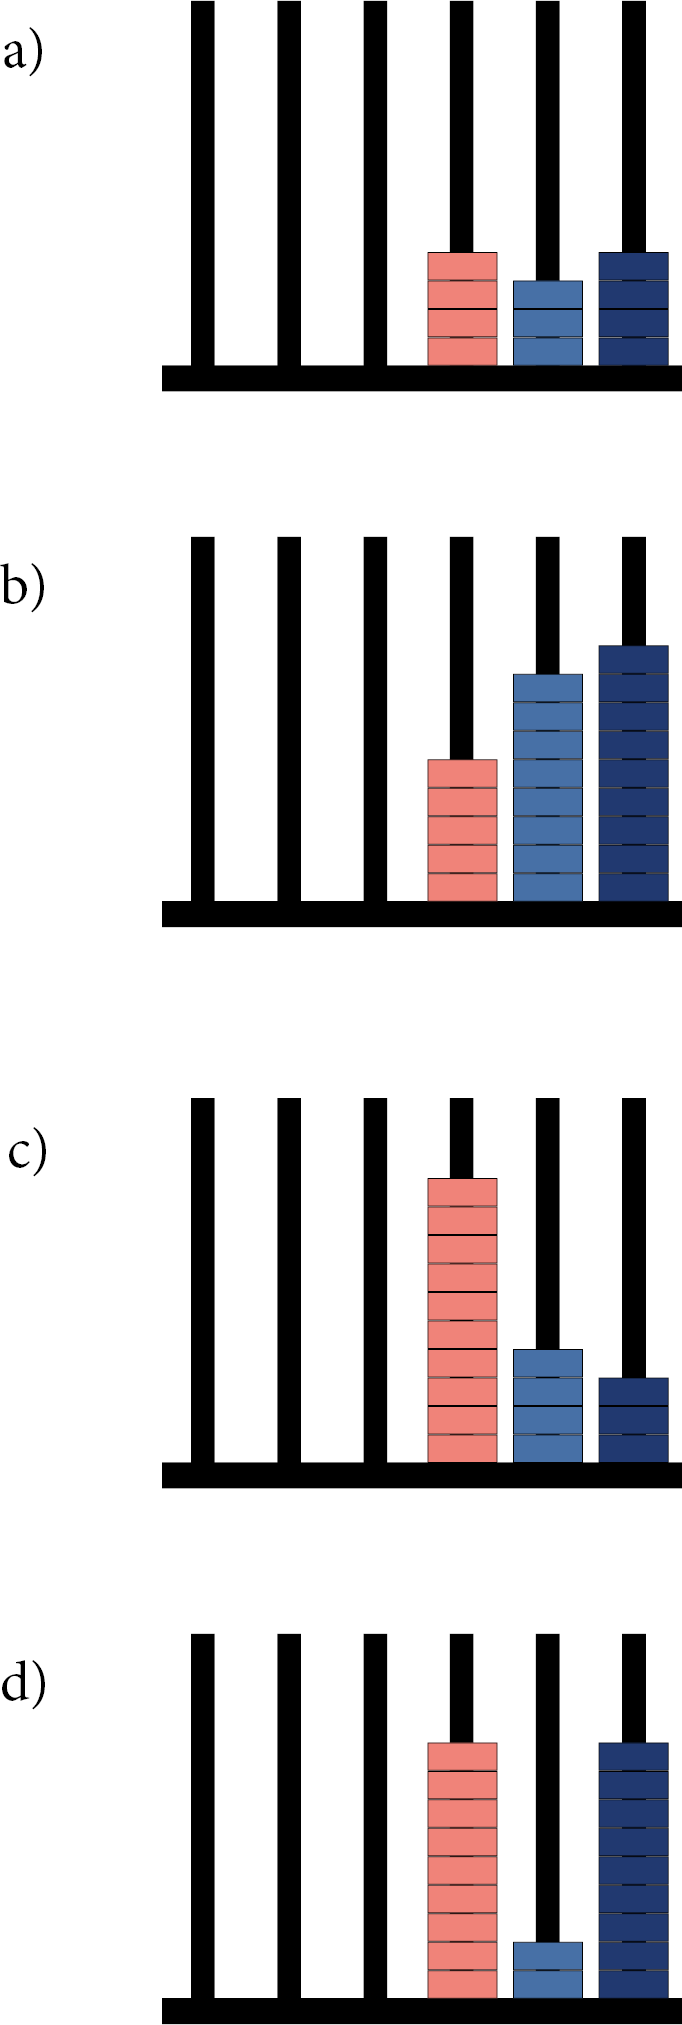
\includegraphics[width=1.25000in,height=0.78248in]{media/image16.png}\tabularnewline
\midrule
\endhead
A & B & C & D\tabularnewline
553 & 425 & 513 & 326\tabularnewline
\bottomrule
\end{longtable}

\begin{longtable}[]{@{}llll@{}}
\toprule
\textbf{1°} & \textbf{2°} & \textbf{3°} & \textbf{4°}\tabularnewline
\midrule
\endhead
D & B & C & A\tabularnewline
\bottomrule
\end{longtable}

Oriente os alunos a descobrirem os números, antes de ordená-los.

\subparagraph{5. }\label{section-4}

É dada a seguinte sequência numérica: 236, 541, 698, 147, 852 e 321. Pinte os
ábacos a seguir, ordenando essa sequência corretamente, de forma
decrescente.

\textless{}Inserir as figuras dos ábacos em branco, conforme o modelo
abaixo.\textgreater{}

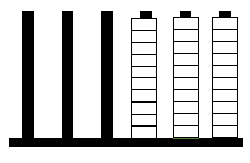
\includegraphics[width=2.03125in,height=1.32438in]{media/image17.png}

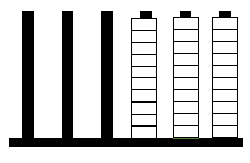
\includegraphics[width=2.03125in,height=1.32438in]{media/image17.png}

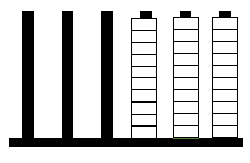
\includegraphics[width=2.03125in,height=1.32438in]{media/image17.png}

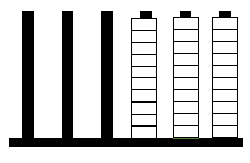
\includegraphics[width=2.03125in,height=1.32438in]{media/image17.png}

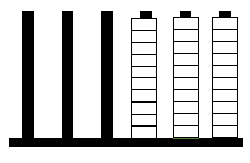
\includegraphics[width=2.03125in,height=1.32438in]{media/image17.png}

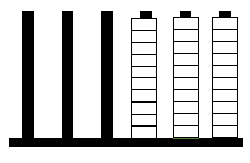
\includegraphics[width=2.03125in,height=1.32438in]{media/image17.png}

A sequência correta, ordenada de forma decrescente, é: 852,
698, 541, 321, 236 e 147. Oriente os alunos a preencherem o ábaco,
considerando a primeira coluna à direita, como representante da ordem
das unidades.

\subparagraph{6. }\label{section-5}

Descubra a charada. Eu sou um algarismo. Se adicionarem o meu valor à
segunda ordem no número 3~927, da direita para a esquerda, os números das próximas
ordens serão mudados. Que algarismo eu sou?

\textless{}https://br.freepik.com/vetores-gratis/colecao-de-numeros-dos-desenhos-animados-com-personagens\_2310814.htm\#query=n\%C3\%BAmeros\%20malucos\%20abra\%C3\%A7ado\&position=34\&from\_view=search\&track=ais\textgreater{}

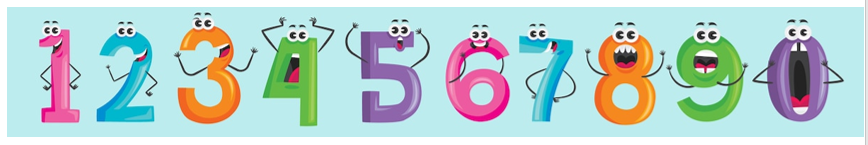
\includegraphics[width=5.90556in,height=0.98611in]{media/image18.png}

\textless{}1 linha\textgreater{}

O aluno deve perceber que, se ele somar o algarismo 8 à
ordem das dezenas, o número obtido será o 4007; logo, as ordens das
centenas e milhares terão seus algarismos modificados. Porém, o
algarismo da ordem das unidades continuará o mesmo.

\subparagraph{7. }\label{section-6}

Dê exemplos de como os números podem ser usados em cada uma das
situações.

\begin{longtable}[]{@{}ll@{}}
\toprule
\begin{minipage}[b]{0.48\columnwidth}\raggedright\strut
Para representar quantidade\strut
\end{minipage} & \begin{minipage}[b]{0.48\columnwidth}\raggedright\strut
\textless{}4 linhas\textgreater{}

Quantidade de pontos de um time de basquete.\strut
\end{minipage}\tabularnewline
\midrule
\endhead
\begin{minipage}[t]{0.48\columnwidth}\raggedright\strut
Para representar ordem\strut
\end{minipage} & \begin{minipage}[t]{0.48\columnwidth}\raggedright\strut
\textless{}4 linhas\textgreater{}

Número de chamada dos alunos da classe.\strut
\end{minipage}\tabularnewline
\begin{minipage}[t]{0.48\columnwidth}\raggedright\strut
Para representar medida\strut
\end{minipage} & \begin{minipage}[t]{0.48\columnwidth}\raggedright\strut
\textless{}4 linhas\textgreater{}

Valor do comprimento de uma régua.\strut
\end{minipage}\tabularnewline
\begin{minipage}[t]{0.48\columnwidth}\raggedright\strut
Para representar código\strut
\end{minipage} & \begin{minipage}[t]{0.48\columnwidth}\raggedright\strut
\textless{}4 linhas\textgreater{}

Número na camisa de jogadores de futebol.\strut
\end{minipage}\tabularnewline
\bottomrule
\end{longtable}

Tente estimular os próprios alunos a citarem diferentes exemplos. Caso, porém, eles não consigam fazê-lo de forma autônoma, ajude-os, mostrando você mesmo a eles os exemplos.

\subparagraph{8. }\label{section-7}

Jorge estava correndo uma maratona em sua cidade. Ele começou a corrida
na posição 63. Na primeira metade da corrida, ele ultrapassou 18
competidores. Na segunda metade, o cansaço chegou; logo, ele foi
ultrapassado por 5 desses competidores que ele havia ultrapassado antes.
Mas, perto do fim da corrida, Jorge juntou forças, começou a correr como
nunca e ultrapassou mais 25 corredores, antes de cruzar a linha de
chegada. Olhe a tabela e indique qual foi o prêmio de Jorge.

\begin{longtable}[]{@{}ll@{}}
\toprule
1° ao 5° lugar & R\$ 1.000,00\tabularnewline
\midrule
\endhead
6° ao 10° lugar & R\$ 500,00\tabularnewline
11° ao 20° lugar & R\$ 300,00\tabularnewline
21° ao 30° lugar & R\$ 200,00\tabularnewline
A partir do 30° lugar & Não recebe prêmio.\tabularnewline
\bottomrule
\end{longtable}

Jorge chegou à metade da corrida em 45° (\(63 - 18\ \)).

Na segunda metade, ficou em 50° (\(45 + 5\ \)).

No finalzinho, ele cruzou a linha em 25° (\(50 - 25\ \)).

Logo, o prêmio foi de de R\$ 200,00.

\subparagraph{9. }\label{section-8}

Indique quais dos números a seguir estão no caça-palavras. Pinte
as bolas que contêm esses números.

\textless{}Inserir o caça-palavras conforme o modelo abaixo, assim como
as bolas com os números.\textgreater{}

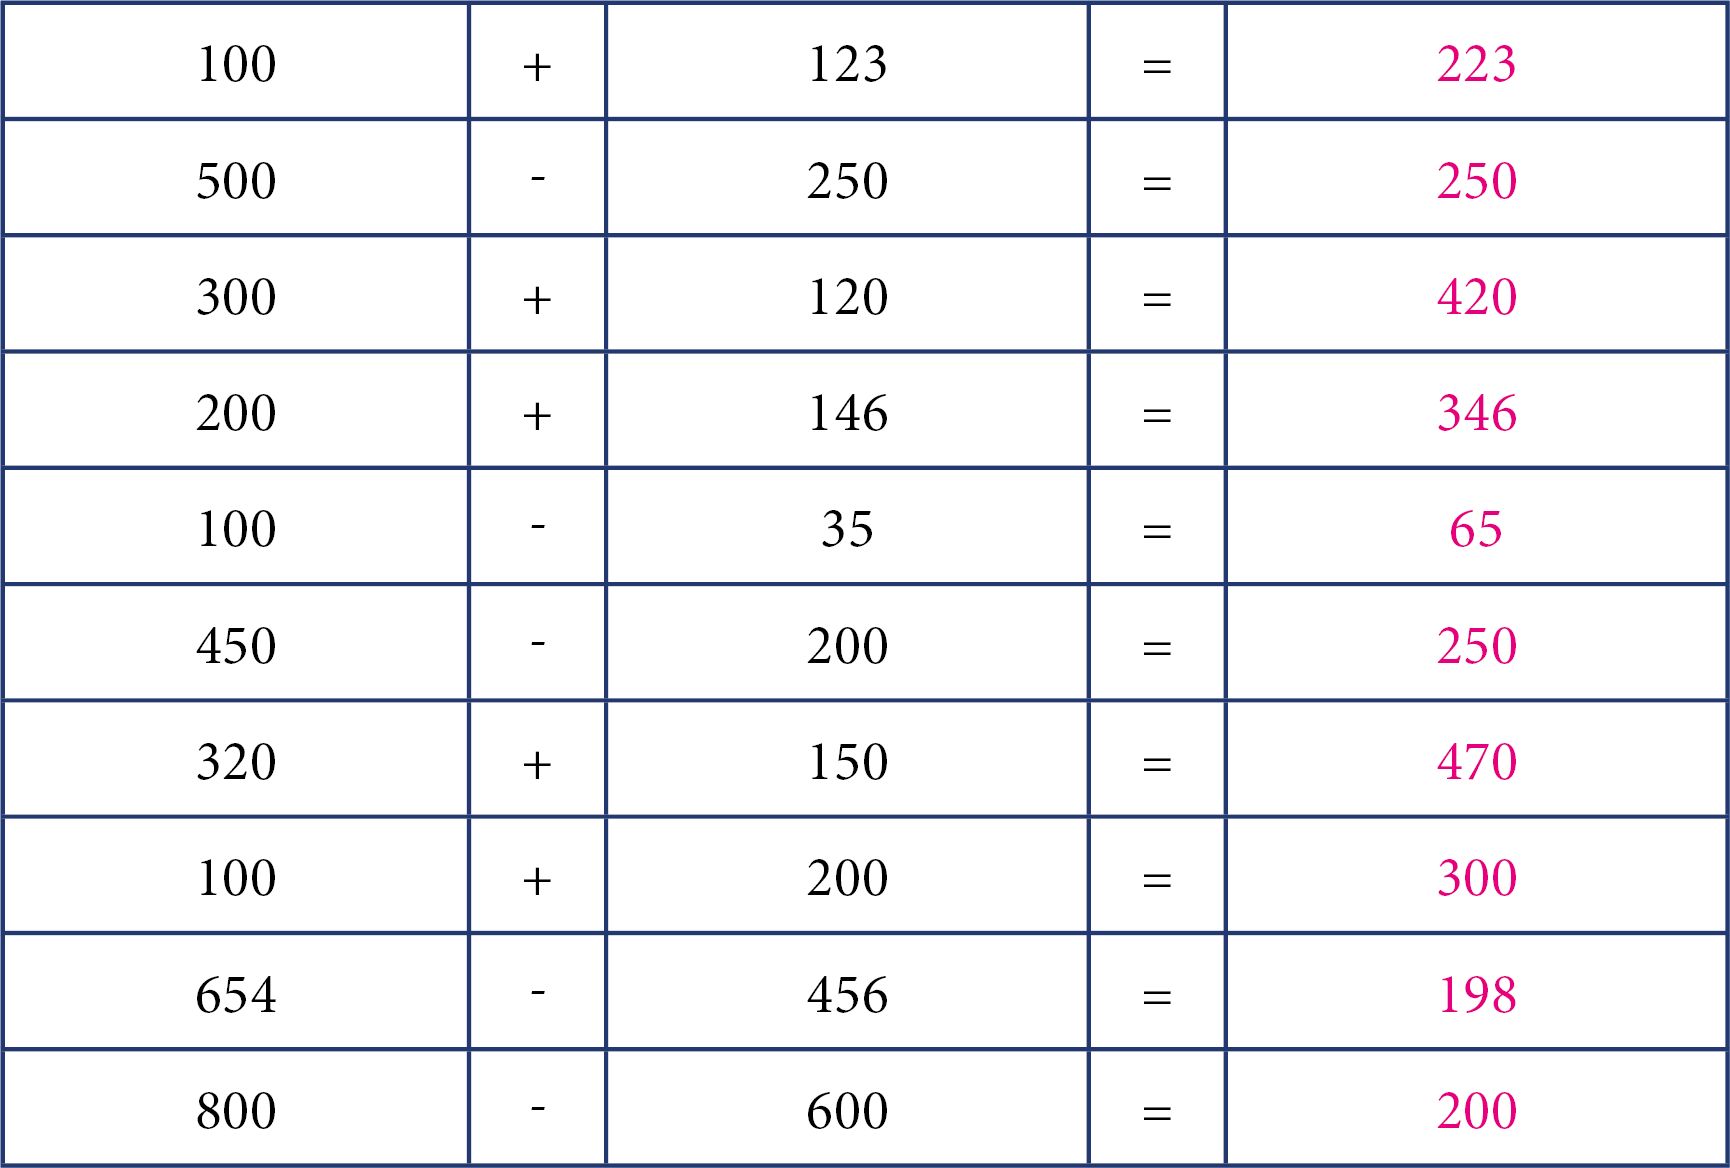
\includegraphics[width=5.00000in,height=3.61458in]{media/image19.png}

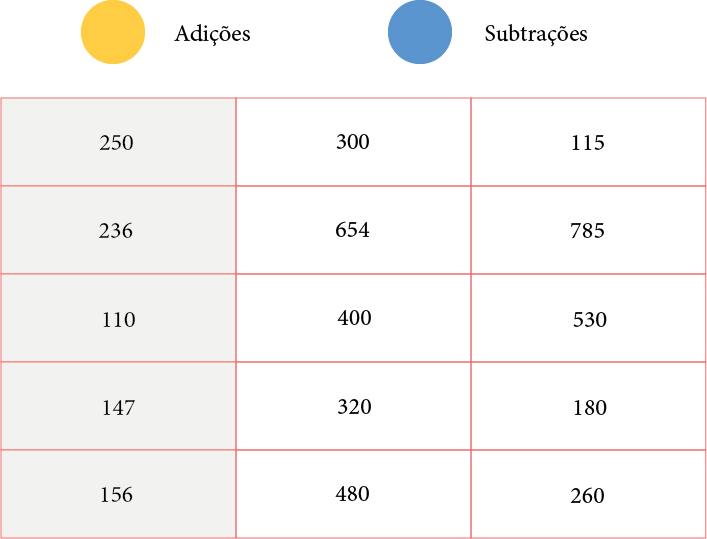
\includegraphics[width=4.35417in,height=1.75000in]{media/image20.png}

Os números encontrados são: 628, 430, 110 e 250.

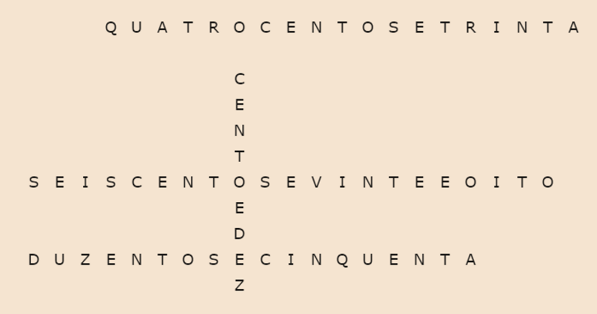
\includegraphics[width=2.71875in,height=1.42734in]{media/image21.png}

\subparagraph{10. }\label{section-9}

Alinhe os estabelecimentos na reta numérica. Escreva o nome dos
estabelecimentos nos quadrados correspondentes, depois de ler o texto.

\textless{}Inserir uma reta numérica com quadrados e marcações, conforme
o modelo a seguir.\textgreater{}

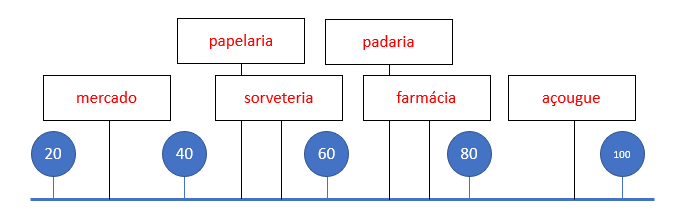
\includegraphics[width=6.36364in,height=2.11458in]{media/image22.png}

Uma padaria fica entre os números 60 e 100 de determinada rua. Já a
farmácia fica entre a padaria e o açougue. A sorveteria fica no número
46, logo após a papelaria. O mercado fica antes da papelaria.

\subparagraph{11. }\label{section-10}

Analise os números e preencha a tabela com as informações pedidas.

\textless{}Inserir um painel com os seguintes números. Eles devem ser
grandes. Inserir uma tabela conforme o modelo a seguir.\textgreater{}


\includegraphics[width=2.72103in,height=2.51437in]{media/image23.png}

\begin{longtable}[]{@{}lll@{}}
\toprule
\begin{minipage}[b]{0.32\columnwidth}\raggedright\strut
Ordem\strut
\end{minipage} & \begin{minipage}[b]{0.32\columnwidth}\raggedright\strut
Quantidade de

números ímpares\strut
\end{minipage} & \begin{minipage}[b]{0.32\columnwidth}\raggedright\strut
Quantidade de

números pares\strut
\end{minipage}\tabularnewline
\midrule
\endhead
Unidades & 5 & 4\tabularnewline
Dezenas & 5 & 4\tabularnewline
Centenas & 6 & 3\tabularnewline
\bottomrule
\end{longtable}

Oriente os alunos a contarem a quantidade de números pares
e ímpares em cada ordem de cada número apresentado nas bolas.

\paragraph{Treino}\label{treino}

\subparagraph{1.}\label{section-11}

A senha do cartão de crédito é um número que indica um(a):

A) código de identificação.

B) medida.

C) quantidade.

D) ordem.

SAEB: Reconhecer o que os números naturais indicam em diferentes
situações: quantidade, ordem, medida ou código de identificação.

BNCC: EF02MA01 - Comparar e ordenar números naturais (até a ordem de
centenas) pela compreensão de características do sistema de numeração decimal (valor
posicional e função do zero).

a) Correta. A senha do cartão identifica o dono do cartão para que não
haja fraudes.

b) Incorreta. A senha do cartão de crédito não mede nenhuma grandeza.

c) Incorreta. A senha do cartão de crédito não quantifica nenhum grupo de objetos.

d) Incorreta. A senha do cartão de crédito não segue uma ordem lógica e sequencial.

\subparagraph{2. }\label{section-12}

Indique qual é o 30° número par entre os números 0 e 100.

A) 30

B) 40

C) 60

D) 90

SAEB: Identificar a posição ordinal de um objeto ou termo em uma sequência (1º, 2º etc.).

BNCC: EF02MA01 - Comparar e ordenar números naturais (até a ordem de centenas) pela compreensão de características do sistema de numeração decimal (valor
posicional e função do zero).

a) Incorreta. O aluno não entendeu que teria que diferenciar entre pares
e ímpares.

b) Incorreta. O aluno indicou o 20° número ao invés do 30°.

c) Correta. Como temos a metade de números pares, basta multiplicar o 30 por 2.

d) Incorreta. O aluno indicou o 45° número ao invés do 30°.

\subparagraph{3. }\label{section-13}

Qual dos ábacos a seguir representa um número com algarismo ímpar na ordem
das dezenas.

\textless{}Inserir as figuras dos ábacos em cada alternativa, conforme
os modelos.\textgreater{}

A) 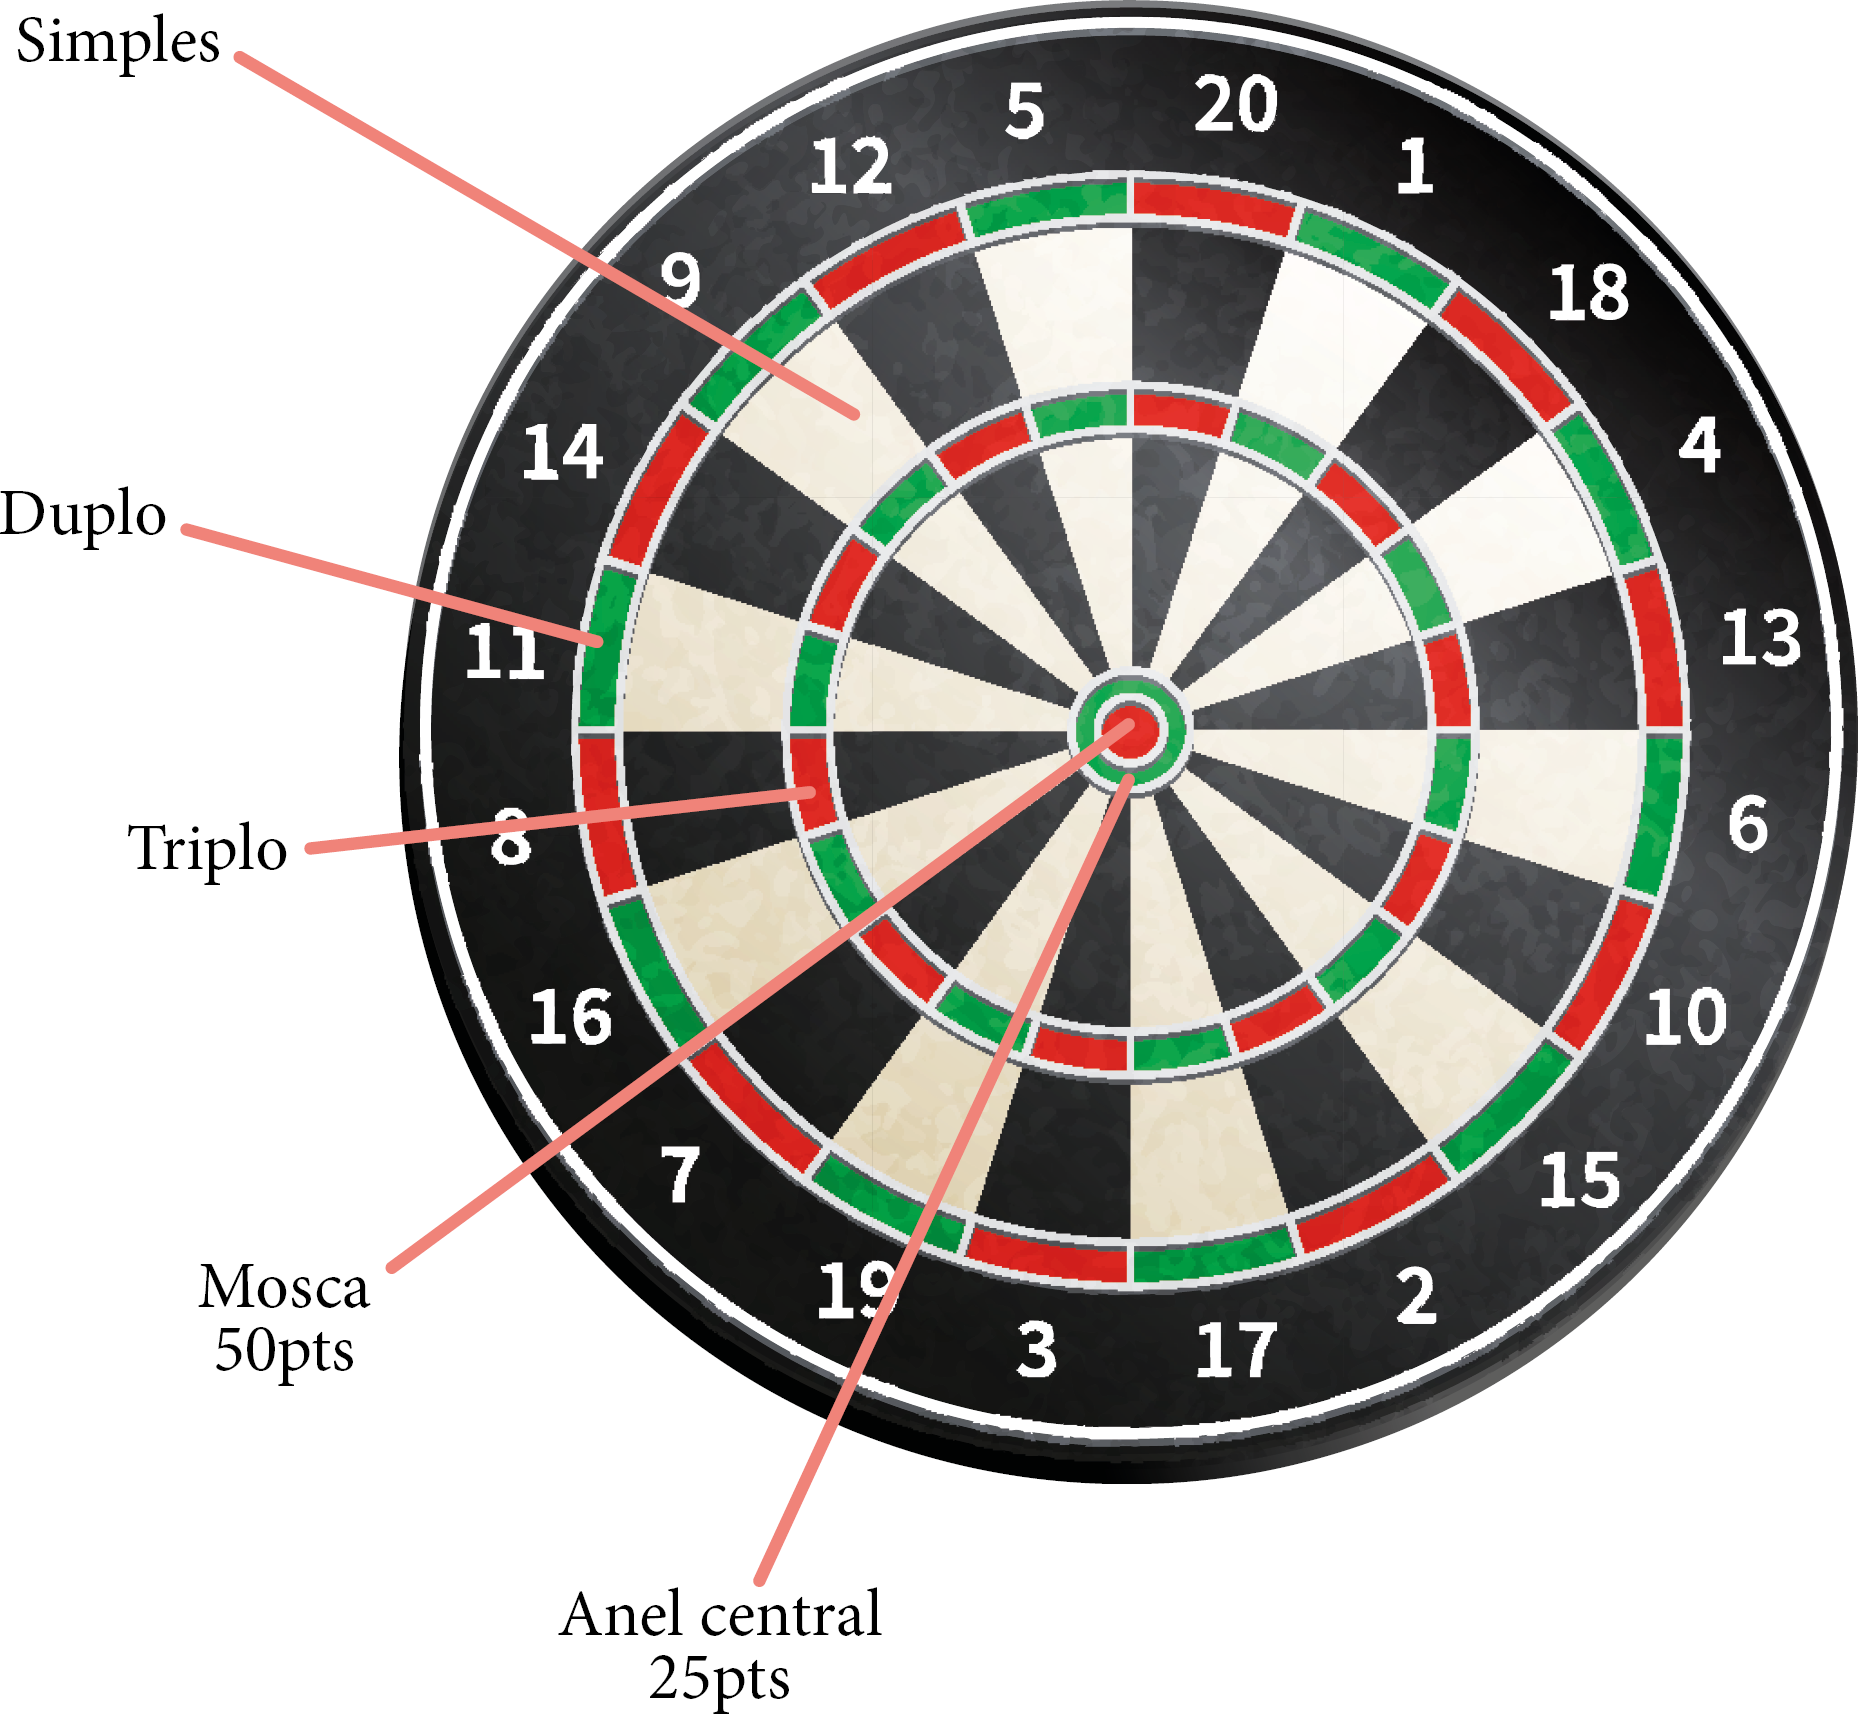
\includegraphics[width=1.42708in,height=0.93377in]{media/image24.png}

B) 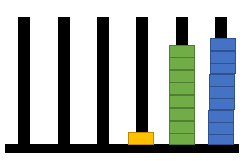
\includegraphics[width=1.43685in,height=0.93657in]{media/image25.png}

C) 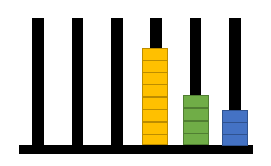
\includegraphics[width=1.41667in,height=0.86777in]{media/image26.png}

D) 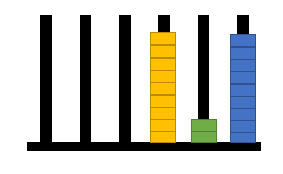
\includegraphics[width=1.45702in,height=0.89583in]{media/image27.png}

SAEB: Identificar a ordem ocupada por um algarismo ou seu valor posicional (ou valor relativo) em um número natural de até 3 ordens.

BNCC: EF02MA03 - Comparar quantidades de objetos de dois conjuntos, por estimativa e/ou por correspondência (um a um, dois a dois, entre outros), para indicar ``tem mais'', ``tem menos'' ou ``tem a mesma quantidade'', indicando, quando for o caso, quantos a mais e quantos a menos.

a) Correta. A ordem das dezenas está representeada pelo número 3.

b) Incorreta. A ordem das dezenas está representeada pelo número 8.

c) Incorreta. A ordem das dezenas está representeada pelo número 4.

d) Incorreta. A ordem das dezenas está representeada pelo número 2.

\chapter{Virando figurinhas}
\markboth{Módulo 2}{}

Neste módulo, vamos desenvolver a habilidade de desenvolvimento de cálculos, tanto no sentido de escolher a melhor
estratégia quanto no sentido de resolver o problema. Faremos essa
abordagem de forma abstrata, mas também de forma contextualizada, com o
fim de desenvolver nos alunos a motivação para resolverem problemas
reais. 

\colorsec{Habilidades do SAEB}
\begin{itemize}
\item Calcular o resultado de adições e subtrações, envolvendo números naturais de até 3 ordens.
\item Compor ou decompor números naturais de até 3 ordens por meio de diferentes adições.
\item Resolver problemas de adição ou de subtração, envolvendo números
naturais de até 3 ordens, com os significados de juntar, acrescentar, separar ou retirar.
\end{itemize}

\colorsec{Habilidades da BNCC}

\begin{itemize}
\item EF02MA04, EF02MA06.
\end{itemize}

\paragraph{Conteúdo}\label{conteuxfado-1}

\textless{}Criar uma figura de crianças brincando com figurinhas no
chão, conforme modelo abaixo.\textgreater{}

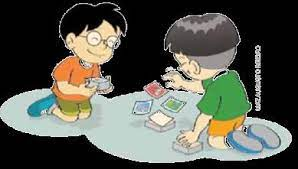
\includegraphics[width=3.10417in,height=1.76042in]{media/image28.png}

Você já jogou bafo? Ou, então, talvez em sua cidade essa brincadeira se
chame tapão! Se já jogou, qual é o seu recorde de virada de figurinhas?
Se nunca ouviu falar, é um jogo em que você tem que deslocar a
maior quantidade de ar possível, fazendo com que um bolo de figurinhas
seja virado. Quem virar mais figurinhas ganha o jogo, e ainda fica com
as figurinhas do seu oponente. A turma toda se junta para competir. Mas
todos precisam ter certeza de quantas figurinhas possuem, para que
ninguém fique com as figurinhas de ninguém por engano. Joel tinha 63
figurinhas de jogadores de futebol, Cristiano tinha mais 43, Eduardo
tinha mais 52 e Ricardo, 81. Eles resolveram apostar tudo e ir
competindo até ver quem ficava com mais figurinhas no final do jogo. Mas,
para isso, eles precisavam adicionar as figurinhas de cada um. Como
eram muitas figurinhas, resolveram fazer pela ordem dos números. Observe
o quadro a seguir.

\begin{longtable}[]{@{}llll@{}}
\toprule
& Centenas & Dezenas & Unidades\tabularnewline
\midrule
\endhead
Joel & & 6 & 3\tabularnewline
Cristiano & & 4 & 3\tabularnewline
Eduardo & & 5 & 2\tabularnewline
Ricardo & & 8 & 1\tabularnewline
\bottomrule
\end{longtable}

Os meninos resolveram separar os números das quantidades de figurinhas
pela ordem. Descobriram que suas figurinhas adicionadas somam 9 unidades
e 23 dezenas. Logo, pensaram: Se temos 23 dezenas, e cada 10 dezenas
formam uma centena, então temos 2 centenas, 3 dezenas e 9 unidades.
Pensando assim, os amigos encontraram a quantidade total de figurinhas, que é de 239.

\paragraph{Atividades}\label{atividades-1}

\subparagraph{1. }\label{section-14}

Complete o quadro a seguir.

\begin{longtable}[]{@{}lllll@{}}
\toprule
100 & + & 123 & = & 223\tabularnewline
\midrule
\endhead
500 & - & 250 & = & 250\tabularnewline
300 & + & 120 & = & 420\tabularnewline
200 & + & 146 & = & 346\tabularnewline
100 & - & 35 & = & 65\tabularnewline
450 & - & 200 & = & 250\tabularnewline
320 & + & 150 & = & 470\tabularnewline
100 & + & 200 & = & 300\tabularnewline
654 & - & 456 & = & 198\tabularnewline
800 & - & 600 & = & 200\tabularnewline
\bottomrule
\end{longtable}

\subparagraph{2. }\label{section-15}

Vamos caçar números? Pinte o resultado das adições e subtrações a seguir,
conforme a cor. Se o número representar o resultado de uma adição, deverá ser pintado de amarelo. Se, por outro lado, ele representar o resultado de uma subtração, ele deverá ser pintado de azul.


\includegraphics[width=3.35417in,height=0.69792in]{media/image29.png}

\begin{longtable}[]{@{}lll@{}}
\toprule
250 & 300 & 115\tabularnewline
\midrule
\endhead
236 & 654 & 785\tabularnewline
110 & 400 & 530\tabularnewline
147 & 320 & 180\tabularnewline
156 & 480 & 260\tabularnewline
\bottomrule
\end{longtable}

\textless{}Inserir uma linha na frente de cada conta
abaixo.\textgreater{}

190 -- 10 = 180

125 + 125 = 250

900 -- 115 = 785

100 + 15 = 115

500 +154 = 654

100 + 10 = 110

300 - 153 = 147

600 -- 200 = 400

600 -- 300 = 300

700 - 220 = 480

250 + 280 = 530

134 + 22 = 156

300 + 20 = 320

190 + 70 = 260

%faltou uma conta aqui: 400 - 164 = 236

\coment {Os números 250, 115, 654, 110, 530, 156, 320 e 260 devem ser pintados de amarelo, porque são resultados de adições. Já os números 180, 785, 147, 400, 300, 480 e 236 devem ser pintados de azul, por representarem subtrações.}

\begin{enumerate}
\def\labelenumi{\arabic{enumi}.}
\setcounter{enumi}{399}
\item
  - 164 = 236
\end{enumerate}

\subparagraph{3.}\label{section-16}

Escreva pelo menos duas formas de compor os números a seguir, utilizando
três parcelas, apenas por meio de adição. Para isso, siga o modelo.

\textless{}Inserir uma linha na frente de cada número.\textgreater{}

500: 250 + 125 + 125 ou 200 + 150 + 150.

650:
\Coment {Sugestão de resposta: 600 + 30 + 20 ou 500 + 100 + 50}

160:
\Coment {Sugestão de resposta: 80 + 70 + 10 ou 50 + 50 + 60}

236:
\Coment {Sugestão de resposta: 200 + 35 + 1 ou 100 + 35 + 101}

129:
\Coment {Sugestão de resposta: 100 + 20 + 9 ou 127 + 1 + 1}

450:
\Coment {Sugestão de resposta: 150 + 150 + 150 ou 300 + 100 + 50}

975:
\Coment {Sugestão de resposta: 900 + 70 + 5 ou 375 + 300 + 300}

135:
\Coment {Sugestão de resposta: 100 + 30 + 5 ou 50 + 50 + 35}

740:
\Coment {Sugestão de resposta: 350 + 350 + 40 ou 400 + 300 + 40}

Os alunos poderão compor os números da forma que quiserem.
Certifique-se de que eles usem pelo menos três parcelas e de que a adição
esteja correta. É dado um exemplo no primeiro número.

\subparagraph{4.}\label{section-17}

Escreva pelo menos duas formas de compor os mesmos números a seguir,
utilizando três parcelas, utilizando somente a subtração. Para isso, siga o modelo.

\textless{}Inserir uma linha na frente de cada número.\textgreater{}

500: 900 -- 200 -- 200 ou 600 -- 50 -- 50.

650:
\Coment {Sugestão de resposta: 1000 -- 300 -- 50 ou 900 -- 150 -- 100}

160:
\Coment {Sugestão de resposta: 300 -- 100 -- 40 ou 200 -- 20 -- 20}

236:
\Coment {Sugestão de resposta: 400 -- 100 -- 64 ou 300 -- 50 -- 14}

129:
\Coment {Sugestão de resposta: 200 -- 70 -- 1 ou 250 -- 71 -- 50}

450:
\Coment {Sugestão de resposta: 900 -- 400 -- 50 ou 500 -- 30 -- 20}

975:
\Coment {Sugestão de resposta: 1000 -- 20 -- 5 ou 2000 -- 1000 -- 25}

135:
\Coment {Sugestão de resposta: 300 -- 100 -- 65 ou 200 -- 50 -- 15}

740:
\Coment {Sugestão de resposta: 900 -- 100 -- 60 ou 1000 -- 200 -- 60}

Os alunos poderão compor os números da forma que quiserem.
Certifique-se de que eles usem pelo menos três parcelas e de que a subtração
esteja correta. É dado um exemplo no primeiro número.

\subparagraph{5.}\label{section-18}

O arco íris é um dos fenômenos mais incríveis da natureza. As cores do
arco-íris se apresentam nesta sequência:

\textless{}
https://br.freepik.com/fotos-gratis/arco-iris-no-ceu-com-paisagem-natural\_34136953.htm\#query=arco\%20\%C3\%ADris\&position=7\&from\_view=search\&track=ais.\textgreater{}

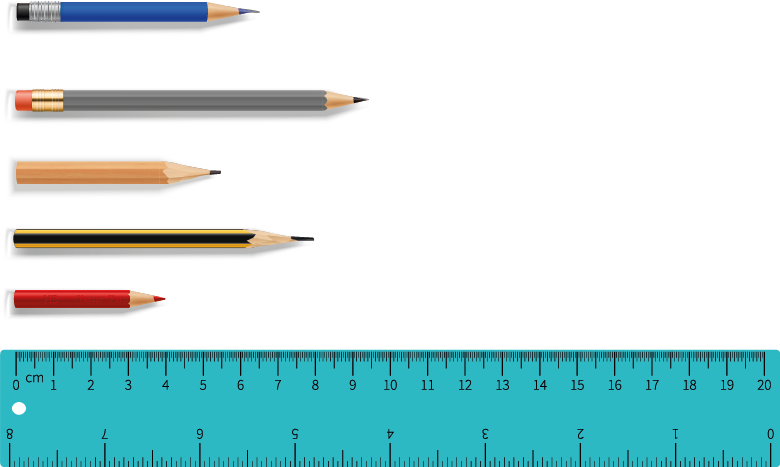
\includegraphics[width=2.40278in,height=3.60417in]{media/image30.png}

\begin{longtable}[]{@{}lllllll@{}}
\toprule
1° & 2° & 3° & 4° & 5° & 6° & 7°\tabularnewline
\midrule
\endhead
Vermelho & Laranja & Amarelo & Verde & Azul & Anil &
Violeta\tabularnewline
\bottomrule
\end{longtable}

Pinte as sete parcelas dos números que compõem o número central na ordem
crescente, conforme a ordem das cores do arco-íris.

\begin{longtable}[]{@{}llllll@{}}
\toprule
10 & 5 & 115 & 6 & 140 & 7\tabularnewline
\midrule
\endhead
48 & 500 & 300 & 400 & 130 & 200\tabularnewline
25 & 20 & 280 & 50 & 60\tabularnewline
410 & 150 & & 120 & 8\tabularnewline
320 & 100 & 30 & 850 & 40 & 70\tabularnewline
280 & 950 & 750 & 9 & 90 & 80\tabularnewline
\bottomrule
\end{longtable}

Os números que podem compor o número 280 em sete parcelas
são: 10, 20, 30, 40, 50, 60 e 70. Esta atividade pode ser feita em
conjunto com a aula de ciências. Auxilie os alunos, pois a atividade
pode exigir um pouco mais deles.

\subparagraph{6.}\label{section-19}

Jogar dardos é muito divertido. Considerando uma rodada com três arremessos no alvo representado, qual a pontuação
máxima em um jogo?

\textless{}Inserir uma imagem de um alvo de dardos simples conforme o
modelo abaixo.\textgreater{}

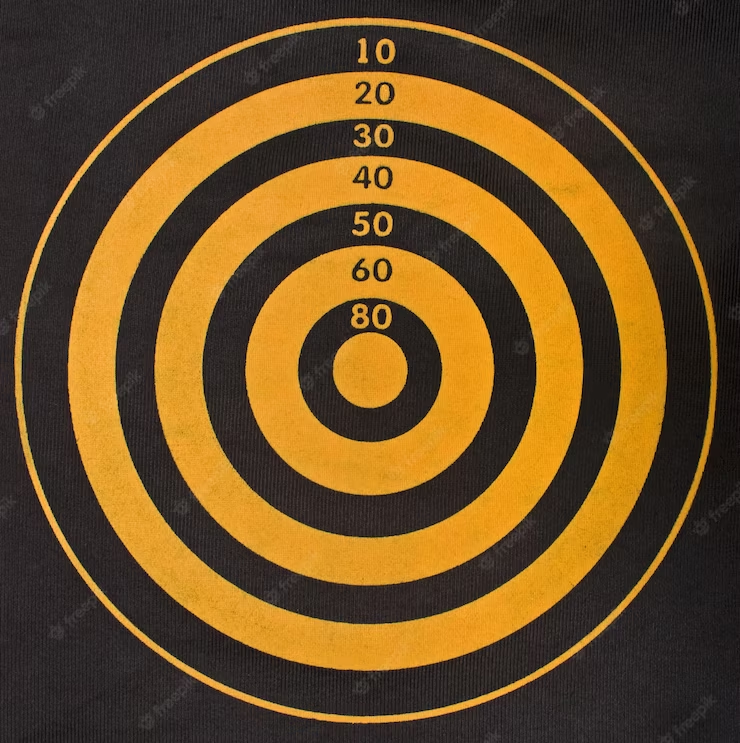
\includegraphics[width=3.78624in,height=3.80208in]{media/image31.png}

Como o alvo identifica a pontuação máxima como 80, logo,
em uma rodada de três lançamentos, a pontuação máxima será 80 + 80 + 80 =
240 pontos.

\subparagraph{7.}\label{section-20}

Ainda pensando nos jogos de dardos, analise a explicação da figura a seguir.

\textless{}
https://dmtoys.com.br/manuais/DM6128\_manual.pdf\textgreater{}

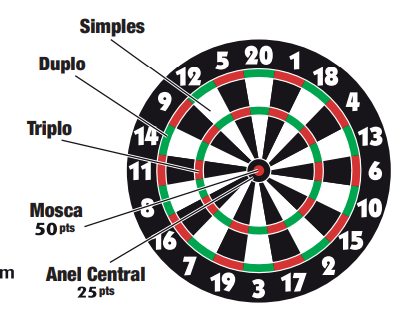
\includegraphics[width=4.23958in,height=3.41667in]{media/image32.png}

Professor, é importante que você explique a pontuação dessa roleta. Não
é difícil de entender, porém, os alunos podem ter dificuldade de
interpretar a figura. Explique que, quando o dardo acerta as faixas finas marcadas em vermelho e verde, há pontuações extras: pontos duplicados no caso do verde e triplicados no caso do vermelho.

Calcule a pontuação das jogadas a seguir, onde os ``x'' azuis mostram onde o dardo acertou o alvo.

https://br.freepik.com/vetores-premium/alvo-de-dardos-classico\_25927311.htm\#page=2\&query=dardos\&position=43\&from\_view=search\&track=sph

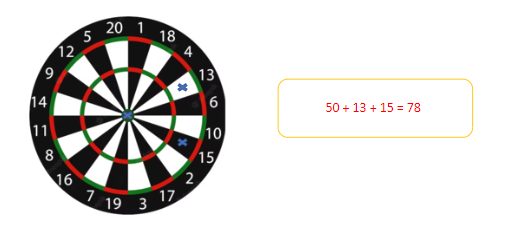
\includegraphics[width=4.77085in,height=2.36458in]{media/image33.png}

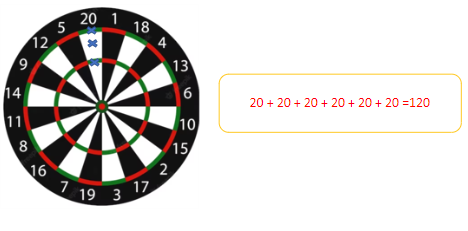
\includegraphics[width=4.87500in,height=2.40625in]{media/image34.png}


\includegraphics[width=4.60417in,height=2.33333in]{media/image35.png}

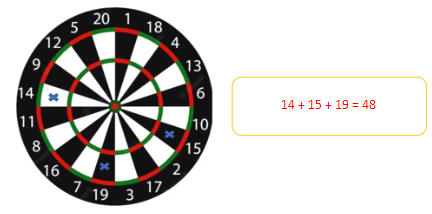
\includegraphics[width=4.50000in,height=2.22917in]{media/image36.png}

\subparagraph{8.}\label{section-21}

Marque, com três x, uma forma de fazer 100 pontos, utilizando 3 dardos no alvo a seguir.

\textless{}Criar uma ilustração do alvo, porém, somente com os
contornos, sem as áreas pintadas de preto, para que o aluno possa
preencher com x. \textgreater{}

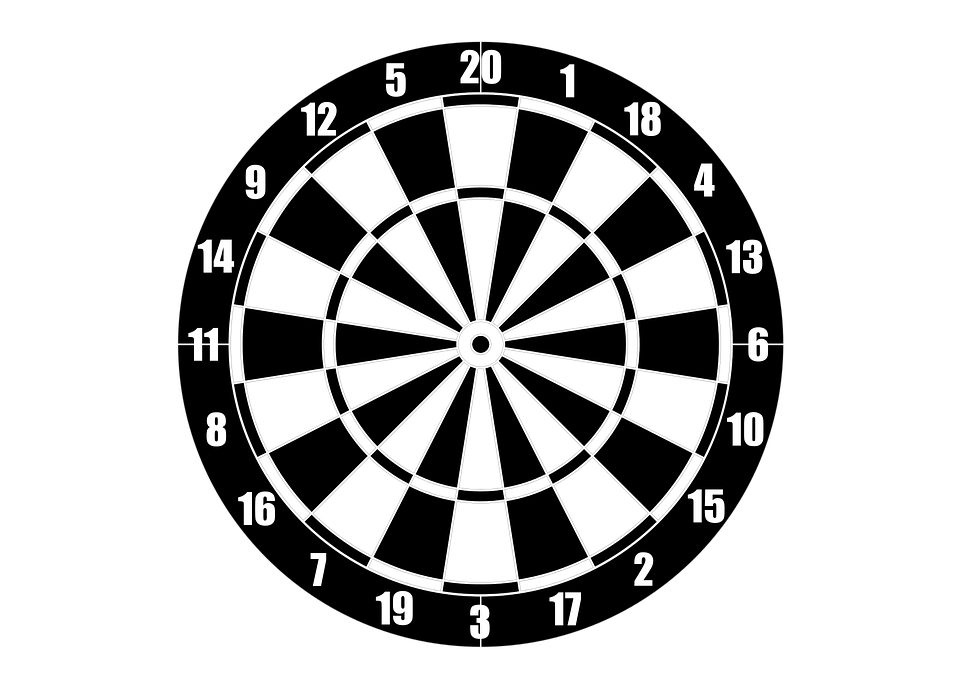
\includegraphics[width=5.00000in,height=3.54167in]{media/image37.png}

Temos várias combinações possíveis. Uma sugestão seria um
dardo no meio (50), outro dardo no duplo 20 e outro no simples 10.

\subparagraph{9.}\label{section-22}

Encontre no caça-palavras 4 números que, juntos, formam o número
570.

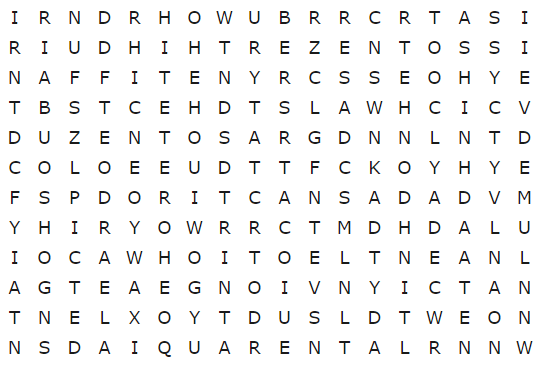
\includegraphics[width=6.04167in,height=4.07813in]{media/image38.png}

Os números são duzentos, trezentos, quarenta e trinta. Ainda que os
alunos não saibam quais são os números, não existem outros no caça
palavras que não seja pertencente as parcelas do número 570. Portanto,
deixe que eles procurem os números, e, depois peça a eles que confiram a
adição.

\subparagraph{10.}\label{section-23}

Em um jogo de virar figurinhas, João apostou suas 24 figurinhas e Marcelo apostou suas 29. Na hora da disputa, João virou 15 figuras e Marcelo virou o resto. Responda o que
se pede:

\begin{enumerate}
\def\labelenumi{\Alph{enumi})}
\item
  Com quantas figurinhas Marcelo ficou? \textless{}2
  linhas\textgreater{}
\end{enumerate}

Primeiro, adicionamos as figurinhas de João e Marcelo: 24 + 29 = 53

Depois retiramos as figuras que João virou do total: 53 - 15 = 38

\begin{enumerate}
\def\labelenumi{\Alph{enumi})}
\item
  Quantas figurinhas João perdeu? \textless{}2 linhas\textgreater{}
\end{enumerate}

Retiramos as figuras que João tirou da quantidade que tinha antes da
disputa: 24 -- 15 = 9

\begin{enumerate}
\def\labelenumi{\Alph{enumi})}
\item
  Quantas figuras Marcelo ganhou? \textless{}2 linhas\textgreater{}
\end{enumerate}

Retiramos as figuras que Marcelo tinha antes da disputa do total que
ganhou: 38 -- 29 = 9

O aluno poderia deduzir que, como o total de figurinhas era a soma das
figurinhas dos dois, antes da disputa, o que João perdeu é exatamente o
mesmo valor que Marcelo ganhou.

\subparagraph{11.}\label{section-24}

Carlinhos tem uma coleção de 56 chaveiros. Ele guarda todos esses
chaveiros em uma caixa de papelão e em um pote de plástico. Eles estão
divididos por temas. Os da caixa de papelão são de times de futebol e os
do pote de plástico são de marcas de carros. Carlinhos resolveu colocar
todos no pote de plástico; logo, retirou os 35 chaveiros que estavam na
caixa de papelão e os colocou no pote. Quantos chaveiros de marcas de
carro Carlinhos tem?

Precisamos retirar a quantidade de chaveiros de times de futebol do
total de chaveiros: 56 -- 35 = 21

\paragraph{Treino}\label{treino-1}

\subparagraph{1.}\label{section-25}

Lucas tem a incrível coleção de 236 \emph{cards} de diversos desenhos
animados. Seu amigo, Leonardo, tem uma coleção um pouco menor, com 132
\emph{cards}. Quantos \emph{cards} os dois têm juntos?

A) 104

B) 366

C) 368

D) 398

SAEB: Resolver problemas de adição ou de subtração, envolvendo
números naturais de até 3 ordens, com os significados de juntar,
acrescentar, separar ou retirar.

BNCC: EF02MA06 - Resolver e elaborar problemas de adição e de subtração, envolvendo números de até três ordens, com os significados de juntar, acrescentar, separar,
retirar, utilizando estratégias pessoais.

a) Incorreta. O aluno subtraiu os números.

b) Incorreta. O aluno errou a adição da ordem das unidades.

c) Correta. A soma dos dois números é igual a 236 + 132 = 368.

d) Incorreta. O aluno errou a adição da ordem das dezenas.

\subparagraph{2. }\label{section-26}

Indique a alternativa que contém uma composição do número 452.

A) 150 + 129 + 173

B) 150 + 139 + 173

C) 150 + 143 + 179

D) 170 + 129 + 183

SAEB: Compor ou decompor números naturais de até 3 ordens por
meio de diferentes adições.

BNCC: EF02MA04 -- Compor e decompor números naturais de até três ordens,
com suporte de material manipulável, por meio de diferentes adições.

a) Correta. A soma dos números resulta em 452.

b) Incorreta. A soma dos números resulta em 462.

c) Incorreta. A soma dos números resulta em 472.

d) Incorreta. A soma dos números resulta em 482.

\subparagraph{3. }\label{section-27}

A região Sul do Brasil tem apenas 3 estados. O Paraná, com 399
municípios; Santa Catarina, com 295 municípios; o Rio Grande do Sul, com
497 municípios. Quantos municípios a região Sul tem no total?

A) 694

B) 792

C) 896

D) 1191

SAEB: Calcular o resultado de adições e subtrações, envolvendo número naturais de até 3 ordens.

BNCC: EF02MA06 -- Resolver e elaborar problemas de adição e de subtração,
envolvendo números de até três ordens, com os significados de juntar, acrescentar, separar,
retirar, utilizando estratégias pessoais.

a) Incorreta. O aluno adicionou somente os municípios do Paraná e de Santa
Catarina.

b) Incorreta. O aluno adicionou somente os municípios de Santa Catarina
e os do Rio Grande do Sul.

c) Incorreta. O aluno adicionou somente os municípios de Paraná e os do Rio
Grande do Sul.

d) Correta. O aluno adicionou corretamente, obtendo: 399 + 295 + 497 = 1191

\chapter{Módulo 3}
\markboth{Módulo 3}{}

Neste módulo, vamos desenvolver as habilidades concernentes
aos conceitos de massa, volume e comprimento. Desenvolver nos alunos a
ideia da necessidade de criarmos padrões de comparação para que medidas
sejam feitas com cada vez mais precisão. 

\colorsec{Habilidades do SAEB}

\begin{itemize}
\item Comparar comprimentos, capacidades ou massas ou ordenar imagens de
  objetos com base na comparação visual de seus comprimentos, capacidades ou massas.
\item Estimar/inferir medida de comprimento, capacidade ou massa de objetos,
  utilizando unidades de medida convencionais ou não, ou medir
  comprimento, capacidade ou massa de objetos.
\item Identificar a medida de comprimento, da capacidade ou da massa de
  objetos, dada a imagem de um instrumento de medida.
\item Reconhecer unidades de medida e/ou instrumentos utilizados para medir
  comprimento, tempo, massa ou capacidade.
\end{itemize}

\colorsec{Habilidades da BNCC}
\begin{itemize}
\item EF02MA16, EF02MA17.
\end{itemize}

\paragraph{Conteúdo}\label{conteuxfado-2}

\textless{}
https://br.freepik.com/fotos-gratis/familia-deitada-na-grama\_1165875.htm\#query=v\%C3\%A1rios\%20p\%C3\%A9s\&position=12\&from\_view=search\&track=ais\textgreater{}

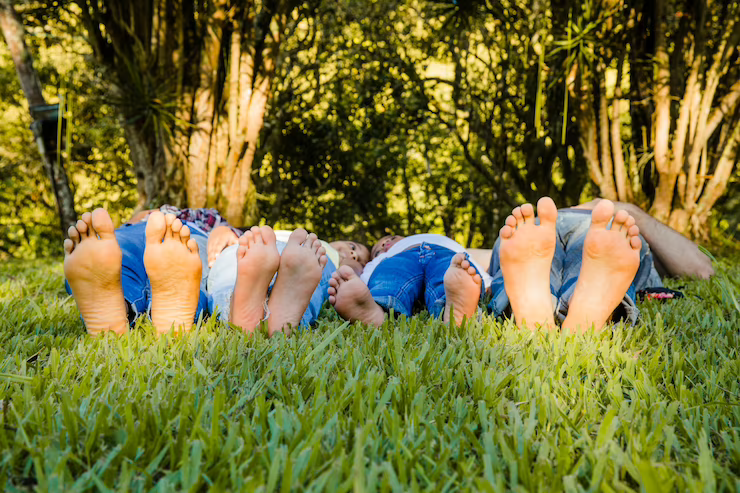
\includegraphics[width=5.00000in,height=1.26043in]{media/image39.png}

Você sabe qual o número do seu sapato? Ou melhor, você sabe qual número você calça? Já ouviu essa pergunta?

Ou, então, já ouviu algum familiar perguntando isso para sua mãe, pois
quer te dar um par de tênis de presente? Pois é! Calçados têm números para
representar os seus tamanhos. Mas como isso é medido? Todos temos
tamanhos padronizados de pés? É claro que não! Cada um de nós tem um
tamanho de pé. Mas, então, como a loja tem sapatos prontos, esperando
para serem vendidos para qualquer um? Existem vários padrões para numerar
um sapato. No Brasil, usamos o mesmo padrão usado na França. Quando
alguém usa um sapato 33, significa que o pé dessa pessoa tem até 21,6
centímetros. A cada 6,6 milímetros, temos um ponto. Vamos lá! Você já
tentou medir seu pé alguma vez? Pegue uma folha e trace o contorno do
seu pé com um lápis ou uma canetinha. Depois, meça do calcanhar até a
ponta do dedão em linha reta. Compartilhe as medidas entre os colegas.
Quem será que tem o maior pé? 

\textless{}
https://www.adidas.com.br/tabela\_de\_tamanhos\_adidas.html\textgreater{}

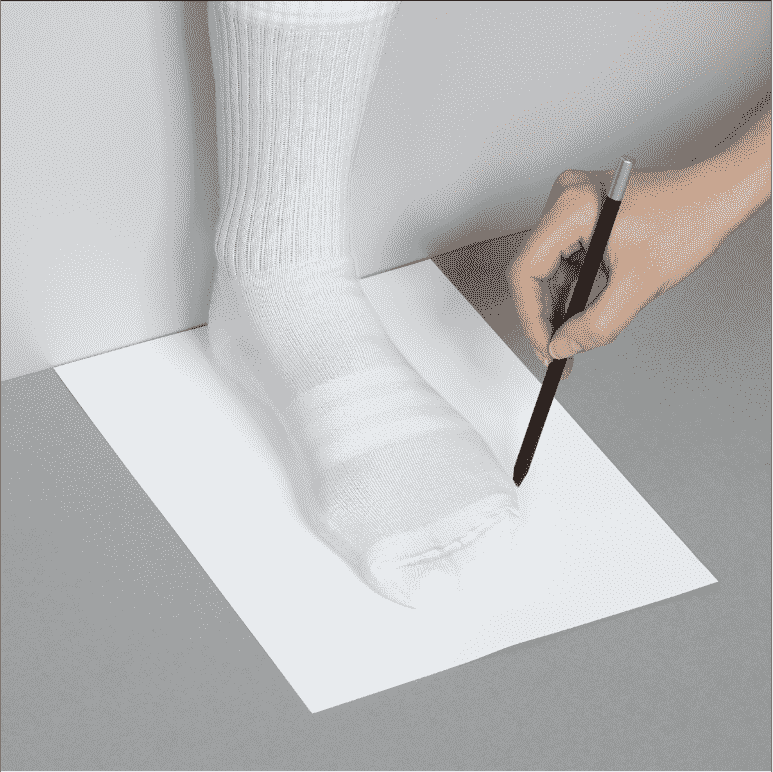
\includegraphics[width=2.47525in,height=2.47010in]{media/image40.png}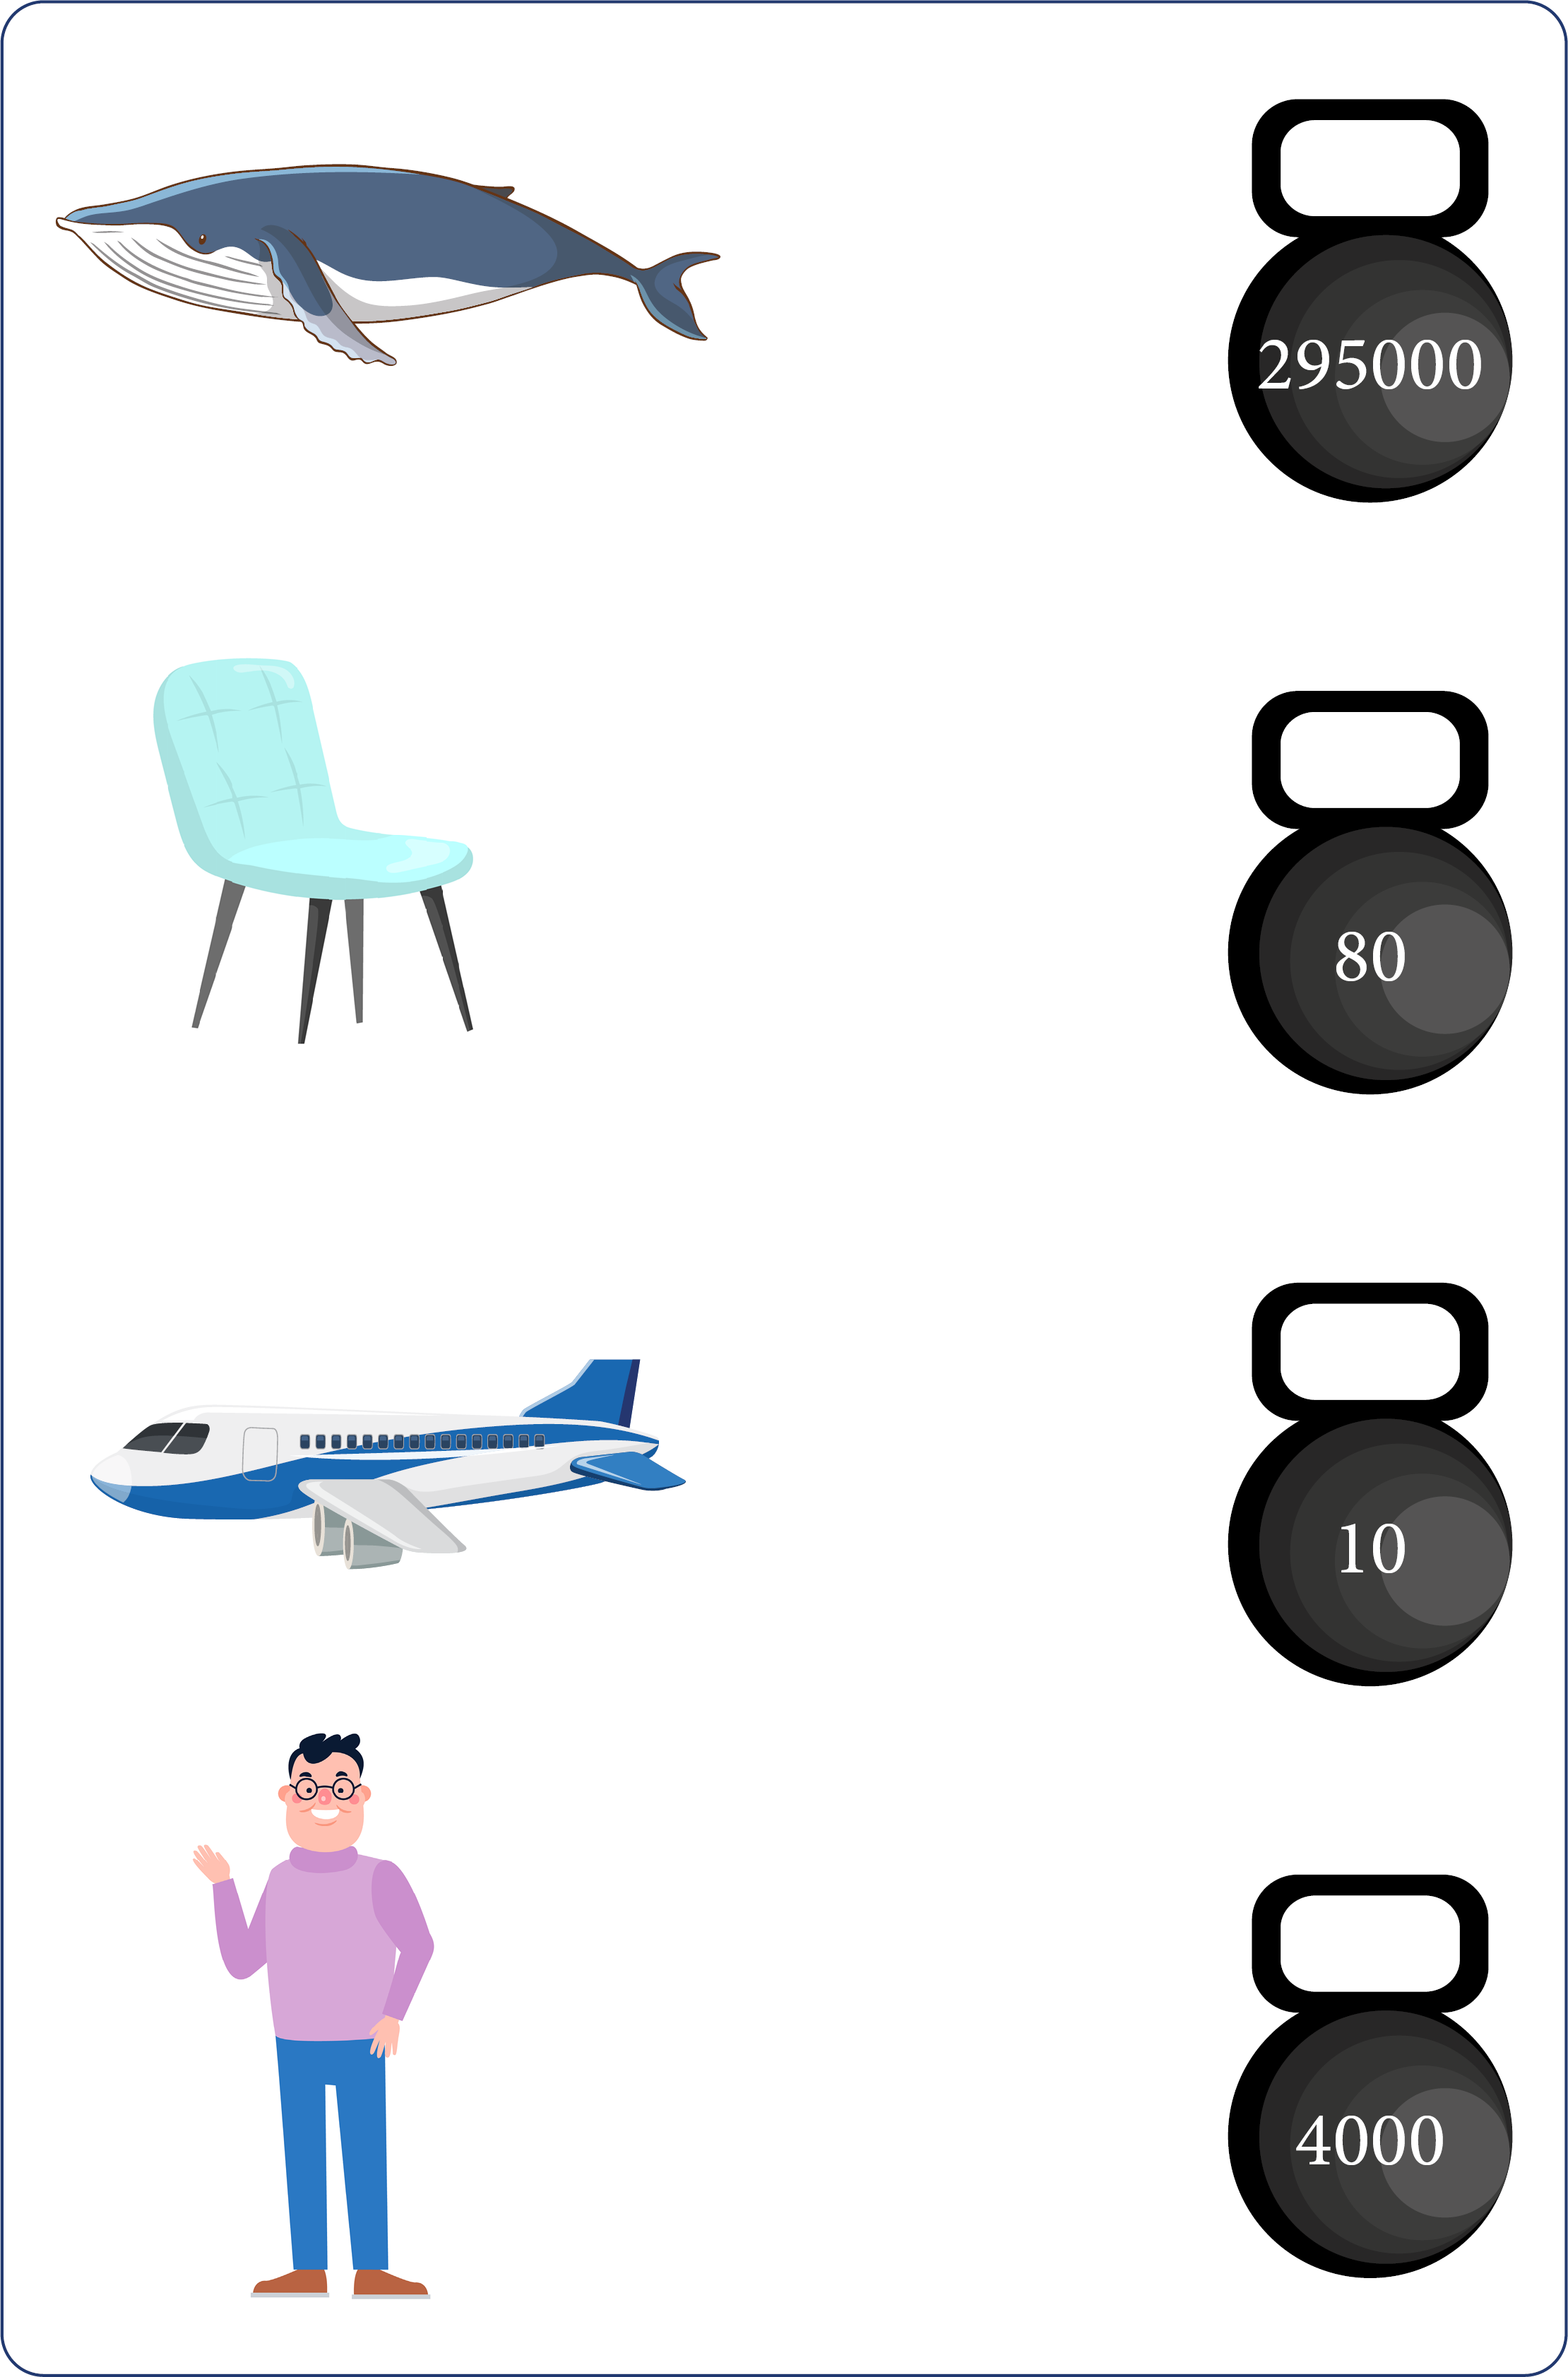
\includegraphics[width=2.51046in,height=2.50000in]{media/image41.png}

\paragraph{Atividades }\label{atividades-2}

\subparagraph{1.}\label{section-28}

Analise a figura e responda:

\textless{}Criar uma figura conforme o modelo a seguir. Essa figura tem
que ocupar um espaço razoável da página para que o aluno consiga
enxergar a escala da régua com facilidade.\textgreater{}


\includegraphics[width=5.76042in,height=3.32424in]{media/image42.png}

\begin{enumerate}
\def\labelenumi{\alph{enumi})}
\item
  Qual cor de lápis tem aproximadamente 9 cm?
\end{enumerate}

\textless{}1 linha\textgreater{}

O lápis de cor verde.

\begin{enumerate}
\def\labelenumi{\alph{enumi})}
\item
  Qual cor de lápis tem aproximadamente 8 cm?
\end{enumerate}

\textless{}1 linha\textgreater{}

O lápis de cor vermelha.

\begin{enumerate}
\def\labelenumi{\alph{enumi})}
\item
  Qual cor de lápis tem aproximadamente 7 cm?
\end{enumerate}

\textless{}1 linha\textgreater{}

O lápis de cor amarela.

\begin{enumerate}
\def\labelenumi{\alph{enumi})}
\item
  O lápis azul é maior, menor ou igual a 7 cm?
\end{enumerate}

\textless{}1 linha\textgreater{}

O lápis de cor azul é menor do que 7 cm.

\begin{enumerate}
\def\labelenumi{\alph{enumi})}
\item
  O lápis rosa é maior, menor ou igual a 3 cm?
\end{enumerate}

\textless{}1 linha\textgreater{}

O lápis de cor rosa é maior do que 3 cm.

\subparagraph{2.}\label{section-29}

Analise a figura, leia o texto e responda ao que se pede.

\textless{}https://br.freepik.com/vetores-gratis/fundo-de-edificio-de-escritorio-moderno\_2850420.htm\#page=2\&query=pr\%C3\%A9dios\&position=26\&from\_view=search\&track=sph\textgreater{}

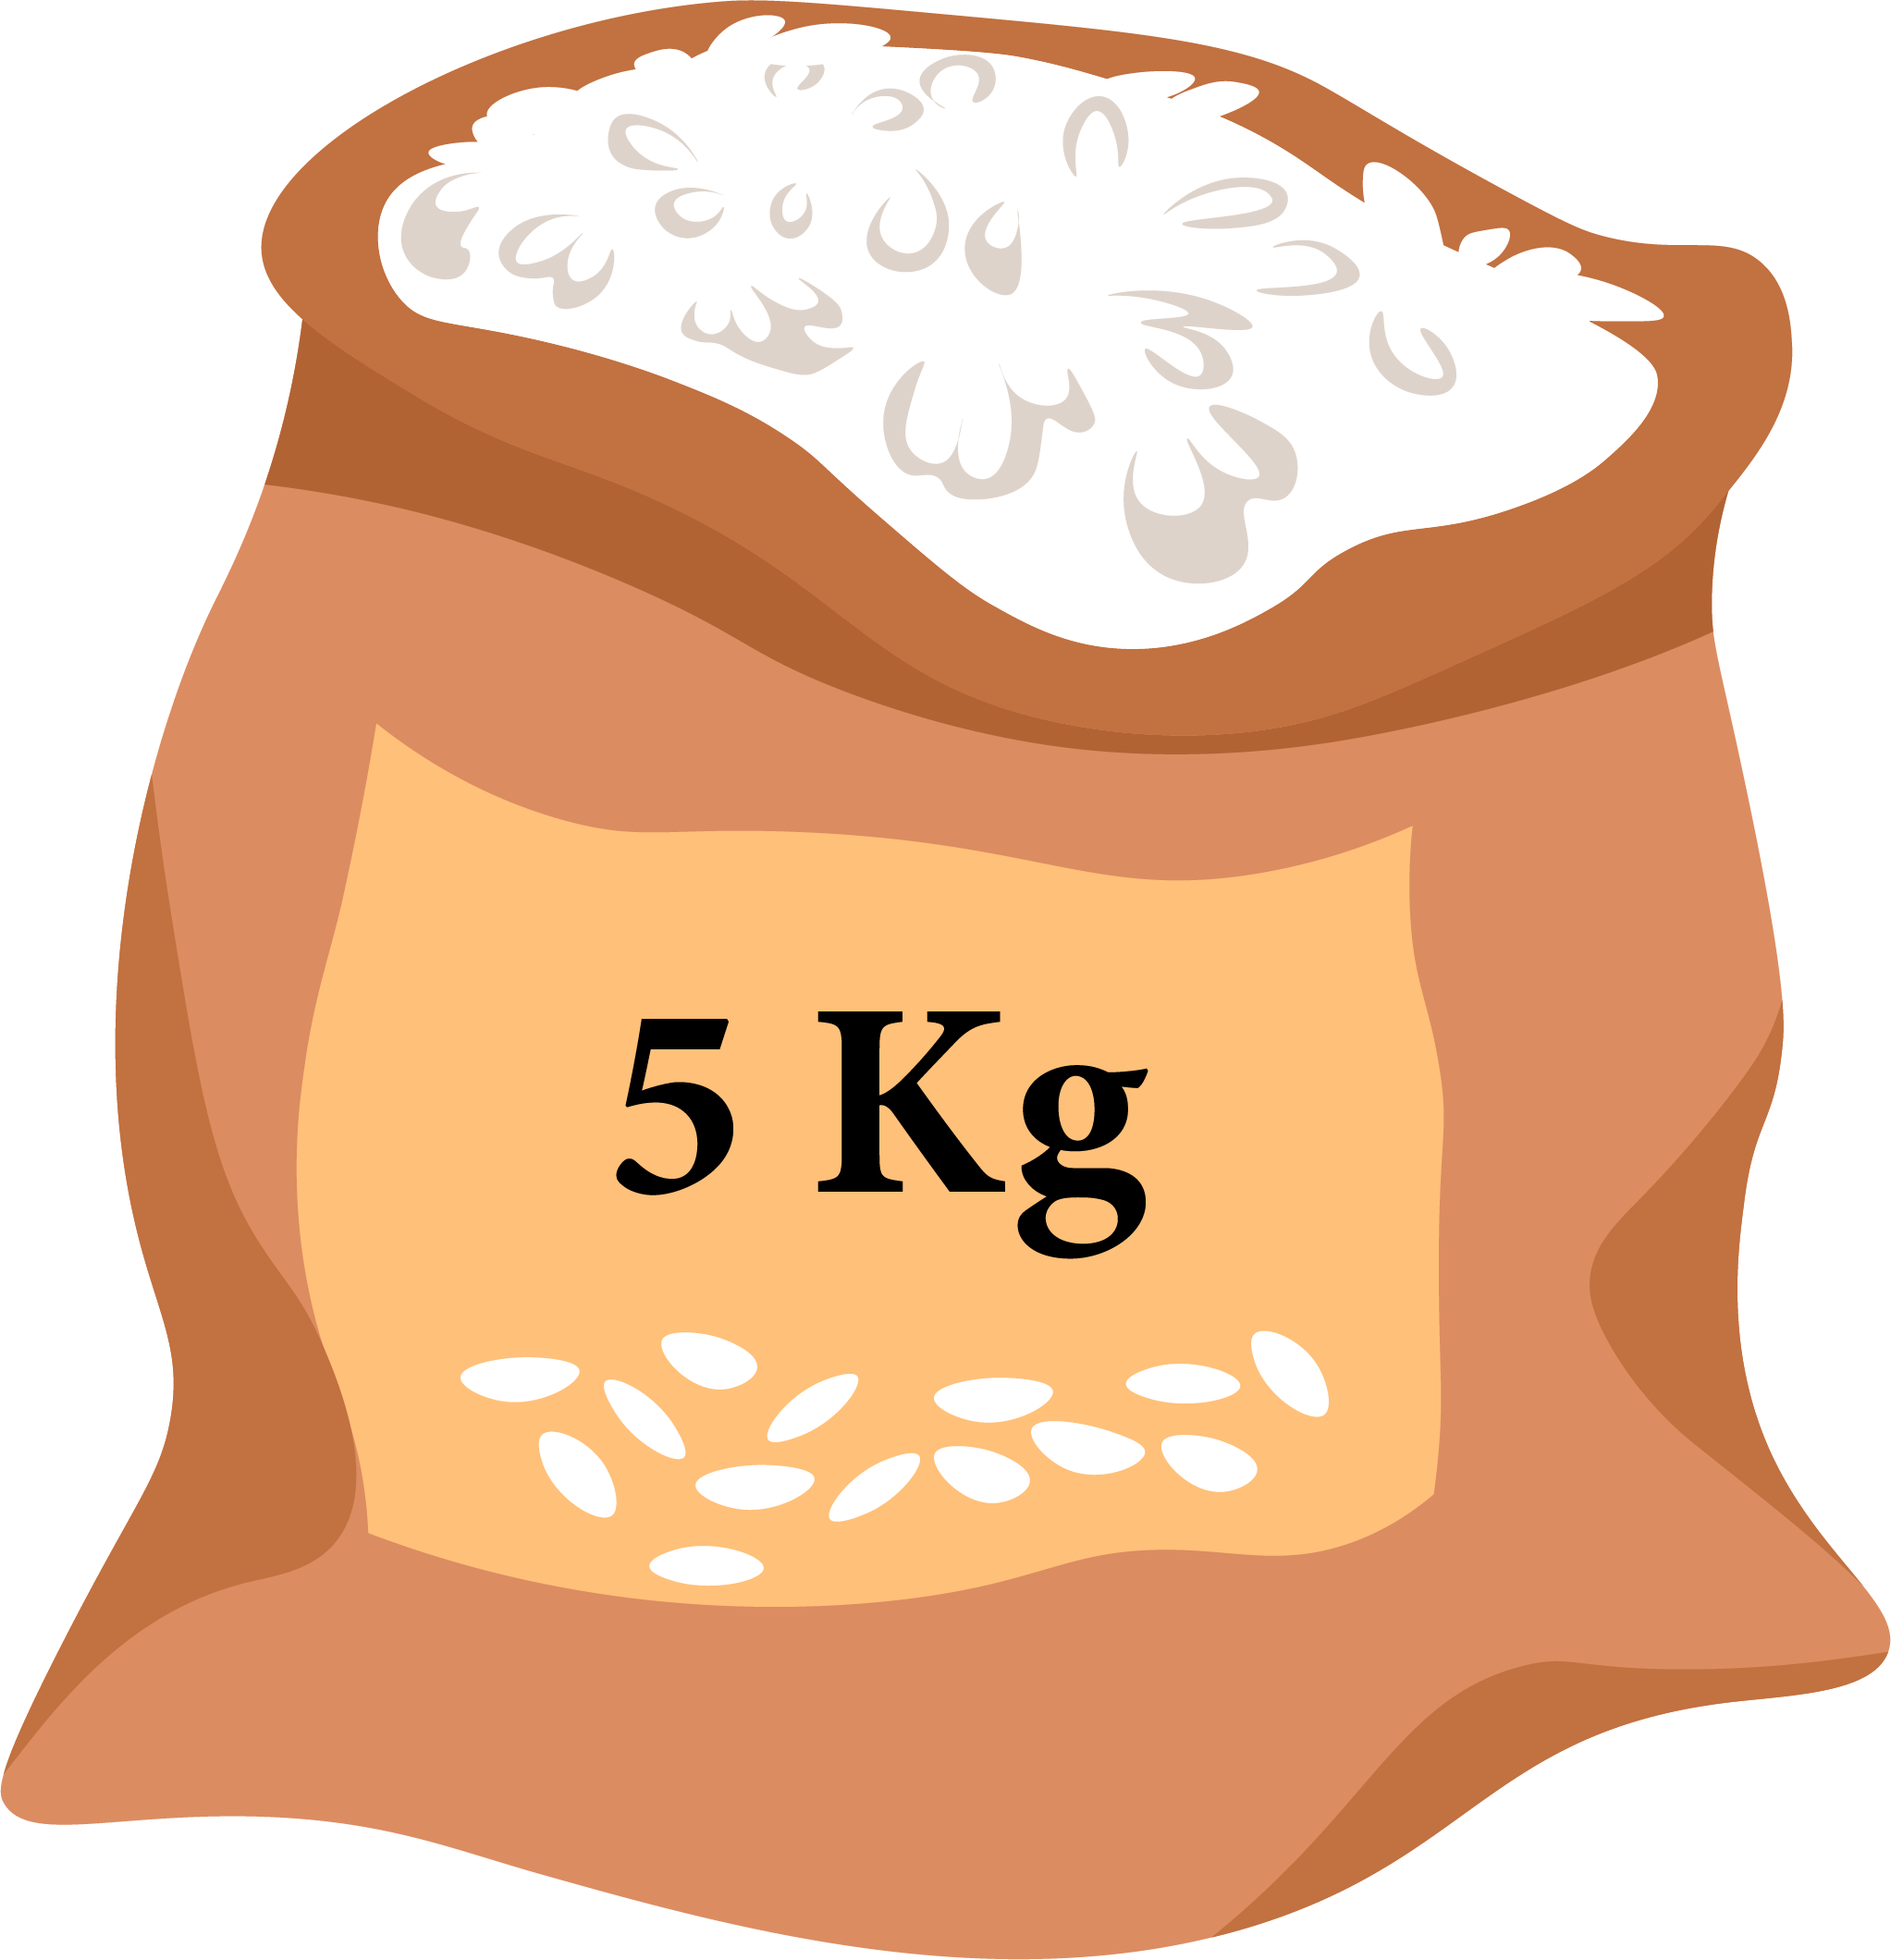
\includegraphics[width=4.31250in,height=2.59651in]{media/image43.png}

O prédio mais alto tem 50 metros de altura; o segundo prédio mais alto
tem 40 metros de altura; os dois prédios que parecem ser do mesmo
tamanho têm 30 metros de altura e o prédio roxo é o mais baixo entre
todos eles.

Qual é o tamanho aproximado do prédio mais baixo, na sua opinião?
Explique como chegou a essa conclusão.

\textless{}4 linhas\textgreater{}

Espera-se que o aluno estime um valor próximo de 20
metros, caso perceba que os prédios vão diminuindo de 10 e 10 metros no
texto. Como eles têm que explicar como chegaram à conclusão, essa
atividade pode ser importante para desenvolver a habilidade de escrever
suas próprias ideias.

\subparagraph{3.}\label{section-30}

Se a pessoa da figura ganhar 10 quilogramas, ficará com que massa?

\textless{}
https://br.freepik.com/vetores-gratis/ilustracao-de-perda-de-peso-de-mulher\_6086077.htm\#query=balan\%C3\%A7a\%20medindo\&position=5\&from\_view=search\&track=ais\textgreater{}

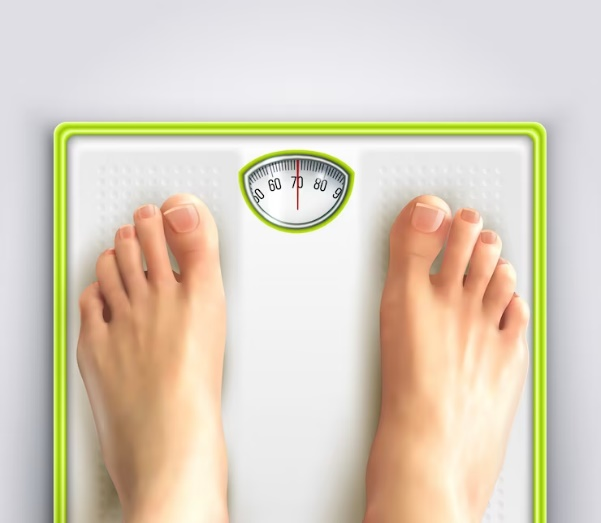
\includegraphics[width=2.72917in,height=2.37665in]{media/image44.jpeg}

\textless{}1 linha\textgreater{}

\begin{enumerate}
\def\labelenumi{\arabic{enumi}.}
\setcounter{enumi}{80}
\item
  g, uma vez que a balança mede atualmente 70 kg.
\end{enumerate}

\subparagraph{4.}\label{section-31}

O instrumento da foto, conhecido como gnômon, utiliza a sombra
provocada pelo Sol para marcar suas várias posições ao longo do dia. O
que este instrumento pode medir?

\textless{}https://stock.adobe.com/br/images/id/296536857?get\_facets=1\&order=relevance\&safe\_search=1\&k=gnomon\&clickref=1101lwCPHVin\&mv=affiliate\&mv2=Freepik\&as\_camptype=\&as\_channel=affiliate\&as\_source=partnerize\&as\_campaign=Freepik\&as\_content=api\&as\_audience=srp\&sdid=6WTV6YJ5\textgreater{}

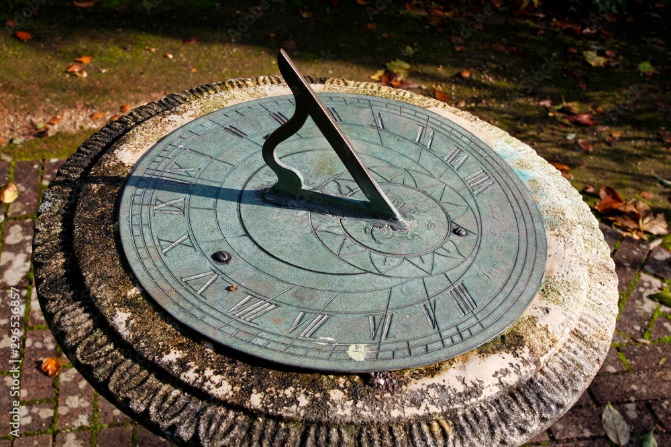
\includegraphics[width=3.05208in,height=2.03472in]{media/image45.jpeg}

\textless{}3 linhas\textgreater{}

Talvez o aluno não perceba que esse instrumento serve para
medir o tempo, uma vez que a ideia de posições pode confundi-lo, ou
induzi-lo a pensar que esse instrumento meça comprimento. É importante,
portanto, utilizar a atividade para mostrar aos alunos que duas
unidades podem ser combinadas para medir outra.

\subparagraph{5.}\label{section-32}

A imagem a seguir mostra três objetos.

\textless{}https://br.freepik.com/fotos-premium/podio-e-produto-de-podio-de-vidro-de-cena-de-palco-na-cena-de-podio-tres-produtos-de-renderizacao-em-3d\_33680968.htm\#query=copos\%20e\%20jarras\%20volume\&position=8\&from\_view=search\&track=ais
Inserir as letras abaixo das figuras.\textgreater{}

\includegraphics[width=3.14583in,height=1.94792in]{media/image46.png}

Compare os objetos e complete o quadro com os valores aproximados.

\begin{longtable}[]{@{}llll@{}}
\toprule
Objeto & A & B & C\tabularnewline
\midrule
\endhead
Capacidade em litros & 1 & 2 & 3\tabularnewline
\bottomrule
\end{longtable}

É importante que o aluno perceba a proporção entre os
objetos e consiga então inferir a capacidade do objeto do meio.

\subparagraph{6.}\label{section-33}

Complete os quadros corretamente, analisando as figuras dos tubos de
ensaio com exames de sangue. Estimando as capacidades ocupadas, indique
quais tubos têm as quantidades informadas no quadro.

%Inserir imagem https://br.freepik.com/fotos-vetores-gratis/sangue-tubo

\includegraphics[width=3.71875in,height=2.70833in]{media/image47.png}

\begin{longtable}[]{@{}lllll@{}}
\toprule
Capacidade ocupada em mL. & 3 & 5 & 6 & 7\tabularnewline
\midrule
\endhead
Letra do tubo & C & B & A & D\tabularnewline
\bottomrule
\end{longtable}

\subparagraph{7.}\label{section-34}

Indique pelo menos duas formas diferentes de medir algo, ou então dois
instrumentos que os meçam:

Comprimento:

\textless{}2 linhas\textgreater{}

Massa:

\textless{}2 linhas\textgreater{}

Capacidade:

\textless{}2 linhas\textgreater{}

Tempo:

\textless{}2 linhas\textgreater{}

Aqui o importante é permitir que os alunos usem a
criatividade e o raciocínio lógico. Alguns exemplos de respostas são:

Comprimento: uma régua e os próprios passos.

Massa: Balança e comparar quantidades da mesma substância que tenha uma
indicação de massa na embalagem, por exemplo.

Capacidade: copos ou seringas.

Tempo: relógio, cronômetro ou até a batida do próprio coração.

\subparagraph{8.}\label{section-35}

Resolva a cruzadinha, descobrindo quais são os instrumentos de medida.

\textless{}Inserir a cruzadinha conforme o modelo abaixo.\textgreater{}

\includegraphics[width=6.14865in,height=2.84375in]{media/image48.png}Horizontais:

1- Ele me diz se estou atrasado, ou se vou chegar a tempo.

3- Ela me diz se engordei ou emagreci, medindo minha massa.

4- Ela me diz o quanto cresci, além de medir o tamanho das coisas.

Verticais:

2- Ela guarda aquilo que mata minha sede, além de me ajudar a medir a
capacidade dos líquidos de ocupar espaço.

As respostas são:

\includegraphics[width=5.00000in,height=2.37500in]{media/image49.png}

\subparagraph{9.}\label{section-36}

Encontre unidades de medidas no caça-palavras.

\includegraphics[width=5.00000in,height=3.32292in]{media/image50.png}

As palavras são: centímetro, mililitro, minutos, quilograma e segundos.

\subparagraph{10.}\label{section-37}

Ligue a figura a sua massa em quilogramas, de forma correta.

\textless{}Inserir um quadro com duas colunas, tendo na coluna da
esquerda as figuras de uma baleia, uma cadeira, um avião e um homem
adulto, e na coluna da direita quatro pesos com as massas indicadas,
conforme o modelo abaixo. Descaracterizar as figuras.\textgreater{}

\includegraphics[width=5.28125in,height=5.51714in]{media/image51.png}

As relações corretas são:

Baleia -- 4.000

Cadeira -- 10

Avião -- 295.000

Homem adulto -- 80

\subparagraph{11.}\label{section-38}

A figura mostra uma balança de ponteiros. Responda ao que se pede.

\textless{}
https://www.istockphoto.com/br/foto/verde-balan\%C3\%A7as-gm95240724-11146949?utm\_source=pixabay\&utm\_medium=affiliate\&utm\_campaign=ADP\_photo\_sponsored\&utm\_content=https\%3A\%2F\%2Fpixabay.com\%2Fpt\%2Fphotos\%2Flibra-balan\%25C3\%25A7a-de-cozinha-2312349\%2F\&utm\_term=waage+k\%C3\%BCchenwaage.
É importante que a figura esteja grande suficiente, para os alunos
enxergarem as graduações\textgreater{}

\includegraphics[width=3.04167in,height=3.04167in]{media/image52.png}

\begin{enumerate}
\def\labelenumi{\alph{enumi})}
\item
  Qual a capacidade máxima da balança, ou seja, qual a maior massa que ela consegue medir?
\end{enumerate}

\textless{}1 linha\textgreater{}

1.000 gramas ou 1 quilograma.

\begin{enumerate}
\def\labelenumi{\alph{enumi})}
\item
  Quanto a balança está medindo na imagem?
\end{enumerate}

\textless{}1 linha\textgreater{}

150 gramas.

\begin{enumerate}
\def\labelenumi{\alph{enumi})}
\item
  Dá pra medir a massa do pacote de arroz da figura nessa
  balança? Explique.
\end{enumerate}

\textless{}https://br.freepik.com/vetores-premium/abra-o-icone-do-saco-de-arroz-pacote-de-tela-de-graos-asiaticos\_28762137.htm.
Acrescentar a medida.\textgreater{}

\includegraphics[width=1.53125in,height=1.43597in]{media/image53.png}

\textless{}2 linhas\textgreater{}

Não dá, pois o saco de arroz tem 4 kg de massa, o que está além da capacidade da balança.

\begin{enumerate}
\def\labelenumi{\alph{enumi})}
\item
  Dá para medir a massa do pacote de café da figura a seguir nessa
  balança? Explique.
\end{enumerate}

\textless{}https://br.freepik.com/vetores-gratis/colecao-dos-elementos-do-cafe\_1076091.htm\#query=caf\%C3\%A9\%20no\%20saco\&position=13\&from\_view=search\&track=ais.
Acrescentar a medida. Substitua coffee bean por café.\textgreater{}

\includegraphics[width=1.32094in,height=1.80208in]{media/image54.png}

\textless{}2 linhas\textgreater{}

Dá para medir, pois a massa do pacote de café tem a metade da capacidade
de medição da balança.

\begin{enumerate}
\def\labelenumi{\alph{enumi})}
\item
  Quanto mede cada risquinho da balança?
\end{enumerate}

\textless{}1 linha\textgreater{}

5 gramas.

\paragraph{Treino}\label{treino-2}

\subparagraph{1.}\label{section-39}

A menina da figura a seguir está usando os braços para medir:

\textless{}
https://br.freepik.com/vetores-premium/a-menina-mede-a-largura-usando-o-estiramento-da-mao\_24777556.htm\#query=medidas\&position=9\&from\_view=search\&track=sph\textgreater{}

\includegraphics[width=3.53125in,height=3.14257in]{media/image55.png}

A) Capacidade

B) Comprimento

C) Massa

D) Tempo

SAEB: Identificar a medida de comprimento, da capacidade ou da
massa de objetos, dada a imagem de um instrumento de medida.

BNCC: EF02MA16 -- Estimar, medir e comparar comprimentos de lados de
salas (incluindo contorno) e de polígonos, utilizando unidades de medida não padronizadas e
padronizadas (metro, centímetro e milímetro) e instrumentos adequados.

a) Incorreta. Os braços da menina não podem calcular o espaço ocupado
pela lousa.

b) Correta. Os braços da menina medem o comprimento entre a borda da
lousa e o ponto marcado.

c) Incorreta. Os braços da menina não podem medir a massa da lousa

d) Incorreta. Os braços da menina não podem calcular o tempo.

\subparagraph{2. }\label{section-40}

A imagem mostra um tubo de ensaio com um líquido vermelho que será estudado.

\textless{}
https://br.freepik.com/fotos-gratis/closeup-tiro-de-um-conta-gotas-em-um-copo-com-um-liquido-vermelho-em-uma-parede-branca\_13006316.htm\#page=3\&query=tubo\%20de\%20ensaio\%20sangue\&position=8\&from\_view=search\&track=ais\textgreater{}

\includegraphics[width=2.00003in,height=3.45840in]{media/image56.png}

Sabendo que dentro do conta-gotas, que é o tubinho menor dentro do tubo
maior, tem 5 mL do líquido vermelho, indique a alternativa que mostra a
quantidade total de líquido vermelho corretamente.

A) Exatamente 10 mL.

B) Pouco menos de 20 mL.

C) Mais de 30 mL.

D) Exatamente 40 mL.

SAEB: Estimar/inferir medida de comprimento, capacidade ou
massa de objetos, utilizando unidades de medida convencionais ou não ou
medir comprimento, capacidade ou massa de objetos.

BNCC: EF02MA17 -- Estimar, medir e comparar capacidade e massa,
utilizando estratégias pessoais e unidades de medida não padronizadas ou padronizadas (litro, mililitro,
grama e quilograma).

a) Incorreta. O marcador do tubo marca bem mais de 10 mL.

b) Incorreta. O marcador do tubo marca mais de 20 mL.

c) Correta. O marcador marca um pouquinho mais do que 40 mL; logo, mesmo que baixasse um pouco o nível com a retirada do conta-gotas, ele subiria novamente acima de 30 mL.

d) Incorreta. É impossível fazer uma estimativa tão precisa nesse caso, apenas com a observação.

\subparagraph{3.}\label{section-41}

A figura mostra o comprimento dos lados do parquinho da escola.
Estime o tamanho do lado A, do lado B, o comprimento total do contorno
do parquinho e, então, indique a resposta.

\textless{}Inserir figura conforme o modelo a seguir.\textgreater{}

\includegraphics[width=3.63542in,height=2.37500in]{media/image57.png}

A) a = 2, b = 5 e c = 7.

B) a = 5, b = 2 e C = 11.

C) a = 5, b = 2 e c = 18.

D) a = 2, b = 5 e c = 18.

SAEB: Comparar comprimentos, capacidades ou massas ou ordenar
imagens de objetos com base na comparação visual de seus comprimentos,
capacidades ou massas.

Estimar/inferir medida de comprimento, capacidade ou massa de
objetos, utilizando unidades de medida convencionais ou não ou medir
comprimento, capacidade ou massa de objetos.

BNCC: EF02MA16 -- Estimar, medir e comparar comprimentos de lados de
salas (incluindo contorno) e de polígonos, utilizando unidades de medida não padronizadas e
padronizadas (metro, centímetro e milímetro) e instrumentos adequados.

a) Incorreta. O aluno inverteu A e B, além de adicionar somente os lados
desconhecidos.

b) Incorreta. O aluno adicionou os lados, mas esqueceu de adicionar os
valores de A e B.

c) Correta. Os lados A e B são iguais aos seus correspondentes e a
adição dos lados é igual a 2 + 2 + 5 + 2 + 2 + 5 = 18.

d) Incorreta. O aluno inverteu os valores de A e B.

\chapter{O juiz apita}
\markboth{Módulo 4}{}

Neste módulo, vamos desenvolver nos alunos a habilidade de
orientar-se no tempo, sabendo identificar o tempo presente, assim como
prever dias e horários de eventos futuros. 

\colorsec{Habilidades do SAEB}

\begin{itemize}
\item Identificar sequência de acontecimentos relativos a um dia.
\item Identificar datas, dias da semana ou meses do ano em calendário ou
escrever uma data, apresentando o dia, o mês e o ano.
\item Determinar a data de início, a data de término ou a duração de um
acontecimento entre duas datas.
\item Determinar o horário de início, o horário de término ou a duração de
um acontecimento.
\end{itemize}

\colorsec{Habilidades da BNCC}

\begin{itemize}
\item EF02MA18, EF02MA19.
\end{itemize}

\paragraph{Conteúdo}\label{conteuxfado-3}

Você já parou pra pensar quanto tempo demora um jogo de um esporte
qualquer? Às vezes vamos jogar bola e não nos damos conta do tempo que
passa. Simplesmente, jogamos até cansarmos, ou então até nossa mãe nos
chamar para entrar. Nos esportes profissionais, porém, não pode ser
assim. Cada modalidade tem o seu tempo determinado. Mas será que temos o
mesmo tempo para todas as modalidades? Será que todas são medidas pelo
tempo? Vamos analisar alguns esportes e compará-los. Veja o quadro.

\begin{longtable}[]{@{}ll@{}}
\toprule
Esporte & Tempo de duração\tabularnewline
\midrule
\endhead
Futebol & São dois tempos de 45 minutos. Tempo total: 1 hora e 30
minutos.\tabularnewline
Basquete & São quatro tempos de 10 minutos. Tempo total: 40
minutos.\tabularnewline
Vôlei & Não tem tempo determinado. Acaba quando o time alcança o número
de pontos.\tabularnewline
Fórmula 1 & É determinado pelo número de voltas, mas uma corrida não
pode passar de 2 horas.\tabularnewline
Handebol & São dois tempos de 30 minutos. Tempo total: 1
hora.\tabularnewline
Tênis & Igual ao vôlei, sem tempo determinado. O jogador deve atingir um
número determinado de pontos.\tabularnewline
\bottomrule
\end{longtable}

O tempo de jogo de cada esporte é pensado de forma a não forçar os
atletas além de suas capacidades físicas. Também é levado em
consideração o espetáculo, afinal de contas todo esporte tem o seu
público, que acompanha os jogos, torce e tem seus jogadores favoritos.

\paragraph{Atividades }\label{atividades-3}


\subparagraph{1.}\label{section-43}

Complete o quadro.

\begin{longtable}[]{@{}ll@{}}
\toprule
Quantos meses tem meio ano? & Resposta: 6\tabularnewline
\midrule
\endhead
Quantos dias têm três semanas? & Resposta: 21\tabularnewline
Quantos dias tem, no máximo, um mês? & Resposta: 31\tabularnewline
Quantos dias tem, no mínimo, um mês? & Resposta: 28\tabularnewline
Quantas semanas têm três meses? & Resposta: 12\tabularnewline
Quantas horas tem uma semana? & Resposta: 168\tabularnewline
\bottomrule
\end{longtable}

\subparagraph{2.}\label{section-44}

Organize as tarefas ou atividades na linha do tempo de um dia, conforme
sua realidade. Preencha os números das atividades na sequência em que acontecem com você. Insira atividades que não estejam listadas nos números que aparecem em branco.

\textless{}Criar uma linha do tempo conforme o modelo a seguir.\textgreater{}

\includegraphics[width=6.59406in,height=1.38750in]{media/image59.png}

\begin{longtable}[]{@{}llll@{}}
\toprule
1 & Acordar & 9 & Brincar com os amigos\tabularnewline
\midrule
\endhead
2 & Tomar banho & 10 & %deixar em branco \tabularnewline
3 & Escovar os dentes & 11 & %deixar em branco \tabularnewline
4 & Tomar café ou lanche & 12 & %deixar em branco \tabularnewline
5 & Almoçar & 13 & Ir para a escola\tabularnewline
6 & Jantar & 14 & %deixar em branco \tabularnewline
7 & Dormir & 15 & %deixar em branco\tabularnewline
8 & Estudar & 16 & Descansar\tabularnewline
\bottomrule
\end{longtable}

A atividade não tem uma resposta determinada, pois dependerá do cotidiano do aluno. O importante é que cada um consiga organizar, na linha do tempo, sua própria rotina, de forma lógica.

\subparagraph{3.}\label{section-45}

Analise o calendário de 2023 e indique o dia da semana dos eventos pedidos.

\textless{} https://7calendar.com/pt/calendar/p-1/ . É importante que o
calendário tome uma folha. \textgreater{}

\includegraphics[width=4.46875in,height=6.30882in]{media/image60.png}

\begin{enumerate}
\def\labelenumi{\alph{enumi})}
\item
  Páscoa - 9 de abril.
\end{enumerate}

\textless{}1 linha\textgreater{}

Domingo.

\begin{enumerate}
\def\labelenumi{\alph{enumi})}
\item
  Dia das Mães - 14 de maio.
\end{enumerate}

\textless{}1 linha\textgreater{}

Domingo.

\begin{enumerate}
\def\labelenumi{\alph{enumi})}
\item
  Independência do Brasil - 7 de setembro.
\end{enumerate}

\textless{}1 linha\textgreater{}

Quinta-feira.

\begin{enumerate}
\def\labelenumi{\alph{enumi})}
\item
  Dia das Crianças - 12 de outubro.
\end{enumerate}

\textless{}1 linha\textgreater{}

Quinta-feira.

\begin{enumerate}
\def\labelenumi{\alph{enumi})}
\item
  Proclamação da República - 15 de novembro.
\end{enumerate}

\textless{}1 linha\textgreater{}

Quarta-feira.

\subparagraph{4.}\label{section-46}

Joaquina foi ao dentista no dia 06 de janeiro de 2023 e fez uma
obturação. O dentista pediu para ela voltar 15 dias depois da primeira
consulta. Sabendo disso, complete o quadro. (Utilize o calendário
da atividade anterior.)

\begin{longtable}[]{@{}ll@{}}
\toprule
PERGUNTAS & RESPOSTAS\tabularnewline
\midrule
\endhead
Em que dia da semana aconteceu a primeira consulta? & Sexta-feira\tabularnewline
Em que dia e mês aconteceu a segunda consulta? & 21 de
janeiro\tabularnewline
Em que dia da semana aconteceu a segunda consulta? &
Sábado\tabularnewline
\bottomrule
\end{longtable}

\subparagraph{5.}\label{section-47}

Todo dia 1° de maio, de todos os anos, comemoramos o Dia do Trabalhador,
assim como todo dia 20 de julho, também de todos os anos, comemoramos o
Dia Internacional da Amizade. Quantos dias se passam entre essas duas
comemorações, sem contar as datas em si?

Permita que os alunos escolham as suas próprias
estratégias para resolverem esse problema. Eles podem simplesmente
contar os dias no calendário, ou tentar fazer isso por meio dos
cálculos, lidando com os dias do mês.

\begin{enumerate}
\def\labelenumi{\arabic{enumi}.}
\setcounter{enumi}{30}
\item
  dias de maio + 30 dias de junho + 19 dias de julho = 79 dias.
\end{enumerate}

\subparagraph{6.}\label{section-48}

Mariana saiu de sua casa às 07h30min e voltou às 11h40min. Marque esses
horários nos relógios, desenhando os ponteiros nas posições
corretas. Em seguida, determine quanto tempo Mariana ficou fora de casa.

\textless{}
https://br.freepik.com/fotos-gratis/relogio-sem-maos\_944733.htm\#query=rel\%C3\%B3gio\%20anal\%C3\%B3gico\&position=0\&from\_view=search\&track=ais\textgreater{}

\begin{longtable}[]{@{}ll@{}}
\toprule
SAÍDA & CHEGADA\tabularnewline
\midrule
\endhead
\includegraphics[width=2.71875in,height=2.65625in]{media/image61.png} &
\includegraphics[width=2.71875in,height=2.65625in]{media/image61.png}\tabularnewline
\begin{minipage}[t]{0.48\columnwidth}\raggedright\strut
Quanto tempo Mariana ficou fora de casa? \textless{}1
linha\textgreater{}

4 horas e 10 minutos.\strut
\end{minipage}\tabularnewline
\bottomrule
\end{longtable}

Os relógios devem ser preenchidos conforme o modelo abaixo:

%Ajustar os ponteiros dos relógios de modelo, porque um deles está errado no modelo, marcando 10h40min em vez de 11h40min.

\includegraphics[width=3.23958in,height=1.57255in]{media/image62.png}

\subparagraph{7.}\label{section-49}

O relógio da figura a seguir mostra o horário em que Rogério entrou em um
site de jogos. As salas de jogos têm sessões \emph{online} que abrirão
conforme o quadro. Indique o horário em que essas salas abrirão.

\textless{}
https://br.freepik.com/vetores-gratis/relogio-de-parede-do-escritorio-com-as-maos-pretas-e-vermelhas-e-mostrador-branco\_3792142.htm\#query=rel\%C3\%B3gio\%20anal\%C3\%B3gico\&position=2\&from\_view=search\&track=ais
\textgreater{}

\includegraphics[width=2.15625in,height=2.15625in]{media/image63.png}

\begin{longtable}[]{@{}ll@{}}
\toprule
1/2 hora depois & 9:40\tabularnewline
\midrule
\endhead
1 hora depois & 10:10\tabularnewline
2 horas depois & 11:10\tabularnewline
3 horas depois & 12:10\tabularnewline
12 horas depois & 9:10 da noite ou 21:10\tabularnewline
\bottomrule
\end{longtable}

\subparagraph{8.}\label{section-50}

Indique qual das figuras a seguir mostra uma atividade aconselhável para
ser feita logo após o almoço, circulando a figura.

\textless{}
https://br.freepik.com/vetores-gratis/menino-escovando-os-dentes-em-pe-perto-da-pia-com-torneira-no-banheiro-rotina-diaria-de-higiene-bucal\_24758387.htm\#query=escovar\%20os\%20dentes\&position=16\&from\_view=search\&track=ais;
https://br.freepik.com/vetores-gratis/menino-deitado-na-cama-contando-ovelhas\_9650026.htm\#query=dormir\&position=6\&from\_view=search\&track=sph;
https://br.freepik.com/vetores-gratis/menino-bonito-jogando-futebol-personagem-de-desenho-animado-isolado\_13374338.htm\#query=jogar\%20bola\&position=1\&from\_view=search\&track=ais;
https://br.freepik.com/vetores-premium/garotinho-fofo-nadando-embaixo-d-agua-nas-ferias-de-verao\_16161583.htm\#query=nadar\&position=5\&from\_view=search\&track=sph;
https://br.freepik.com/vetores-gratis/lavar-as-maos-no-fundo-branco\_8033253.htm\#query=lavar\%20as\%20m\%C3\%A3os\&position=8\&from\_view=search\&track=ais.

\includegraphics[width=5.00000in,height=4.05208in]{media/image64.png}

É importante que o aluno perceba que escovar os dentes é a
melhor coisa a ser feita logo após o almoço. Nadar e jogar bola podem
fazer mal logo após uma refeição. Dormir não fará mal algum, porém, deve
ser feito após a escovação dos dentes. Lavar as mãos vai acontecer
também junto com a escovação, mas o aluno precisa olhar para essa imagem
a associar a lavagem das mãos com a antecedência da refeição. 

\subparagraph{9.}\label{section-51}

O professor de educação física resolveu organizar um campeonato de
handebol na escola. A tabela de jogos está no quadro a seguir.

\begin{longtable}[]{@{}lll@{}}
\toprule
JOGOS & DIA & DIA E MÊS\tabularnewline
\midrule
\endhead
TIME A X TME B & 2° feira & 20 de março\tabularnewline
TIME C X TIME D & 3° feira & 21 de março\tabularnewline
TIME A X TIME D & 4° feira & 22 de março\tabularnewline
TIME C X TIME B & 5° feira & 23 de março\tabularnewline
TIME A X TIME C & 6° feira & 24 de março\tabularnewline
TIME B X TIME D & 6° feira & 24 de março\tabularnewline
DISPUTA DE 3° E 4° & 10 de abril\tabularnewline
FINAL & 15 de abril\tabularnewline
\bottomrule
\end{longtable}

Responda ao que se pede.

\begin{enumerate}
\def\labelenumi{\alph{enumi})}
\item
  Em que dia da semana será a disputa de 3° e 4° lugares?
\end{enumerate}

\textless{}1 linha\textgreater{}

Segunda-feira

\begin{enumerate}
\def\labelenumi{\alph{enumi})}
\item
  Em que dia da semana será a disputa da grande final?
\end{enumerate}

\textless{}1 linha\textgreater{}

Sábado.

\begin{enumerate}
\def\labelenumi{\alph{enumi})}
\item
  Quantos dias se passam do início ao fim do torneio?
\end{enumerate}

\textless{}1 linha\textgreater{}

27 dias.

\begin{enumerate}
\def\labelenumi{\alph{enumi})}
\item
  Quantos dias de jogos teremos?
\end{enumerate}

\textless{}1 linha\textgreater{}

\begin{enumerate}
\def\labelenumi{\arabic{enumi}.}
\setcounter{enumi}{7}
\item
  dias.
\end{enumerate}

\subparagraph{10.}\label{section-52}

O calendário mostra os dias dos meses de novembro e dezembro de
2022. Nesses meses, aconteceu a Copa do Mundo FIFA de futebol. A data
marcada pelo círculo vermelho é o início do torneio, quando jogaram
Equador e Catar. Sabendo que a Copa durou 28 dias, além do dia de abertura, circule o dia da
final entre Argentina e França.

\coment {Deve ser marcado o dia 17 de dezembro como resposta.}

\includegraphics[width=6.01042in,height=3.00521in]{media/image65.png}

%Numerar a atividade a seguir como a atividade de número 11

\begin{enumerate}
\def\labelenumi{\arabic{enumi}.}
\item
  Aproveitando os dados da atividade anterior, responda o que se pede?
\end{enumerate}

\begin{enumerate}
\def\labelenumi{\alph{enumi})}
\item
  Sabendo que o Brasil estreou no quarto dia após a abertura, informe o dia, o
  mês e o dia da semana do primeiro jogo do Brasil.
\end{enumerate}

\textless{}2 linhas\textgreater{}

24 de novembro -- quinta-feira.

\begin{enumerate}
\def\labelenumi{\alph{enumi})}
\item
  Sabendo que o Brasil foi eliminado nas quartas de final, pela Croácia,
  no dia 9 de dezembro, informe quantos dias durou a participação do
  Brasil nessa copa, e o dia da semana da eliminação brasileira.
\end{enumerate}

\textless{}2 linhas\textgreater{}

16 dias -- sexta-feira.

\begin{enumerate}
\def\labelenumi{\alph{enumi})}
\item
  A seleção brasileira goleou a seleção coreana por 4 x 1, quatro dias
  antes de ser eliminada. Em que dia, mês e dia da semana esse jogo
  aconteceu?
\end{enumerate}

\textless{}2 linhas\textgreater{}

\begin{enumerate}
\setcounter{enumi}{5}
\item
  de dezembro -- segunda-feira.
\end{enumerate}

\subparagraph{12.}\label{section-53}

Leandro estava correndo na aula de atletismo e marcando o tempo que
demorou para dar uma volta na pista. Antes de iniciar a volta, ele olhou
para o seu relógio e viu o que se vê na figura.

\textless{}
https://br.freepik.com/vetores-gratis/relogio-de-parede-em-fundo-branco\_22732489.htm\#page=4\&query=rel\%C3\%B3gio\&position=12\&from\_view=search\&track=sph\textgreater{}

\includegraphics[width=2.14583in,height=2.10113in]{media/image66.png}

Leandro começou a correr e, ao terminar a volta, seu treinador lhe
mostrou o marcador de tempo que indicava o seguinte:

\textless{}Inserir a figura do cronômetro, conforme modelo a
seguir\textgreater{}

\includegraphics[width=4.61458in,height=1.43750in]{media/image67.png}

Informe em que horário Leandro cruzou a linha de chegada.

\textless{}1 linha\textgreater{}

Às 03h05min da tarde, ou, então, às 15h05min.

\paragraph{Treino}\label{treino-3}

\subparagraph{1.}\label{section-54}

As Olimpíadas de Tóquio, realizadas entre 23 de julho de 2021 e 08 de
agosto de 2021, duraram quantos dias?

A) 15

B) 16

C) 17

D) 18

SAEB: Determinar a data de início, a data de término ou a
duração de um acontecimento entre duas datas.

BNCC: EF02MA18 -- Indicar a duração de intervalos de tempo entre duas
datas, como dias da semana e meses do ano, utilizando calendário, para planejamentos e organização
de agenda.

a) Incorreta. O aluno contou dois dias a menos.

b) Incorreta. O aluno contou dois dias a menos

c) Correta. O aluno contou corretamente a quantidade de dias.

d) Incorreta. O aluno contou um dia a mais.

\subparagraph{2.}\label{section-55}

No dia 10 de julho, Pedro saiu em viagem de férias com a família. Era
uma segunda-feira. Pedro voltou no dia 20 de julho. Que dia da semana
era?

a) Segunda-feira.

b) Terça-feira.

c) Quarta-feira.

d) Quinta-feira.

SAEB: Identificar datas, dias da semana ou meses do ano em calendário ou escrever uma data, apresentando o dia, o mês e o ano.

BNCC: EF02MA18 -- Indicar a duração de intervalos de tempo entre duas datas, como dias da semana e meses do ano, utilizando calendário, para planejamentos e organização de agenda.

a) Incorreta. Segunda-feira será dia 17.

b) Incorreta. Terça-feira será dia 18.

c) Incorreta. Quarta-feira será dia 19.

d) Correta. Quinta-feira será dia 20.

\subparagraph{3.}\label{section-56}

No início da aula de ciências o relógio da sala estava com o ponteiro
menor no número 9 e o ponteiro maior no número 6. Ao término dessa
aula, o mesmo relógio estava com o ponteiro menor no número
10 e o ponteiro maior no número 3. Qual foi a duração da aula de
ciências?

A) 30 minutos.

B) 45 minutos.

C) 50 minutos.

D) 1 hora.

SAEB: Determinar o horário de início, o horário de término ou a
duração de um acontecimento.

BNCC: EF02MA19 -- Medir a duração de um intervalo de tempo por meio de
relógio digital e registrar o horário do início e do fim do intervalo.

a) Incorreta. O aluno contou 15 minutos a menos.

b) Correta. O aluno contou corretamente 30 minutos até fazer 10 horas,
mais 15 minutos do número 3.

c) Incorreta. O aluno contou 5 minutos a mais.

d) Incorreta. O aluno contou 15 minutos a mais.

\chapter{Banco real}
\markboth{Módulo 5}{}

Neste módulo, vamos desenvolver nos alunos a habilidade de
reconhecerem o valor das cédulas de dinheiro, assim como das moedas, por
meio da identificação de suas cores e dos próprios números que as
representam. Também vamos desenvolver neles a capacidade de
resolverem situações problema que favorecem o trabalho com a Educação financeira, além de revisar as habilidades de aplicação das
operações. 

\colorsec{Habilidades do SAEB}

\begin{itemize}
\item Relacionar valores de moedas e/ou cédulas do sistema monetário
brasileiro, com base nas imagens desses objetos.
\item Resolver problemas que envolvam moedas e/ou cédulas do sistema
monetário brasileiro.
\end{itemize}

\colorsec{Habilidade da BNCC}

\begin{itemize}
\item EF02MA20.
\end{itemize}

\paragraph{Conteúdo}\label{conteuxfado-4}

Você já jogou jogos de tabuleiro? Já jogou algum joguinho em que tenha
que manipular dinheiro? Existem jogos em que você precisa comprar casas
e prédios, existem outros jogos que simulam a vida adulta, com suas
contas e deveres. Nesses jogos, às vezes, você ganha dinheiro; às vezes,
você perde dinheiro, mas o importante é que você precisa pensar na
melhor forma de usar o dinheiro que ganha para ganhar o jogo, ou seja,
terminar o jogo com mais dinheiro do que seus adversários.

\textless{}
https://br.freepik.com/vetores-gratis/jogo-de-negocios-competicao-de-sucesso-jogo-de-tabuleiro-e-empresario-jogo-em-equipe-conceito-estrategia-ideia\_10600417.htm\#page=2\&query=jogo\%20de\%20tabuleiro\%20com\%20dinheiro\&position=29\&from\_view=search\&track=ais.
Apague a inscrição business games. Produzir a imagem de um card
fictício, conforme o modelo da direita.\textgreater{}

\includegraphics[width=3.33025in,height=2.95560in]{media/image68.png}\includegraphics[width=2.16667in,height=3.03125in]{media/image69.png}

Imagine que você estivesse jogando um jogo assim e se deparasse com o seguinte
\emph{card}:

Segundo o card:

1. você gastaria 200 para comprar a casa;
2. toda a vez que outro jogador cair na sua casa, terá que pagar 100 de aluguel;
3. caso você precise vender, saberá que vai
perder 50. 

O que você faria? Ficaria com os 200 ou compraria a casa?

\Coment {Professor, mostre aos alunos as vantagens e as desvantagens de se comprar a casa; explique que os ganhos dependeriam de sorte no jogo e das combinações de dados, mas que, caso a compra fosse feita, se pelo menos dois jogadores parassem na casa, isso já valeria a compra por 200.}

\paragraph{Atividades }\label{atividades-4}

\subparagraph{1.}\label{section-57}

Você se lembra dos animais que representam as cédulas da moeda
brasileira? Preencha o quadro com os valores. Preste bem atenção!
Elas estão embaralhadas.

\begin{longtable}[]{@{}ll@{}}
\toprule
Lobo-guará & 200,00\tabularnewline
\midrule
\endhead
Garça & 5,00\tabularnewline
Tartaruga-marinha & 2,00\tabularnewline
Garoupa & 100,00\tabularnewline
Onça-pintada & 50,00\tabularnewline
Mico-leão-dourado & 20,00\tabularnewline
Arara-vermelha & 10,00\tabularnewline
\bottomrule
\end{longtable}

Talvez os alunos não se lembrem. Ajude-os se necessário. Caso tenha cédulas para eles verem, pelo menos algumas delas, isso pode ser útil.

\subparagraph{2.}\label{section-58}

Alguns anos atrás existia a cédula de 1 real, que tinha um beija-flor
estampado. O governo brasileiro resolveu tirar essa cédula de circulação.

\textless{}
https://www.completei.com/cedulas-nacionais/1a-familia-do-real/1-reais-antonio-palacio-filho-henrique-meirellesfe-c-254\textgreater{}

\includegraphics[width=3.30208in,height=3.08528in]{media/image70.png}

Se você comprasse um objeto de R\$ 12,00 e pagasse com uma nota de R\$
20,00, receberia quantas notas de troco, como a da figura?

\textless{}1 linha\textgreater{}

20,00 -- 12,00 = 8,00; logo, receberia 8 cédulas.

\subparagraph{3.}\label{section-59}

Analise a figura e a situação a seguir e responda ao que se pede.
\textless{}Essa atividade pode conter duas páginas\textgreater{}

\textless{}
https://br.freepik.com/vetores-gratis/processo-de-venda-do-vendedor-da-loja-de-frutas-do-mercado-de-alimentos-estilo-simples-trabalho-profissional-moderno-relacionado-a-objetos-de-trabalho-de-homem-vitrine-caixa-bolsa-maca-banana-laranja-kiwi-uvas-pera-pessoas-trabalham-colecao\_11438819.htm\#query=quitanda\&position=10\&from\_view=search\&track=sph.
Acrescentar os preços conforme o modelo.\textgreater{}

\includegraphics[width=3.55208in,height=3.57292in]{media/image71.png}

Todas as frutas são vendidas por dúzia, ou seja, por 12 unidades, exceto
a melancia, que é vendida por unidade, e a uva, que é vendida por cachos.

O quadro mostra as cédulas de Real que você tem.

\begin{longtable}[]{@{}ll@{}}
\toprule
Cédulas (R\$) & Quantidade\tabularnewline
\midrule
\endhead
100,00 & 1\tabularnewline
50,00 & 1\tabularnewline
10,00 & 3\tabularnewline
5,00 & 5\tabularnewline
2,00 & 10\tabularnewline
\bottomrule
\end{longtable}

\begin{enumerate}
\def\labelenumi{\alph{enumi})}
\item
  Monte uma composição de cédulas para comprar: 1 dúzia de bananas, 1
  dúzia de kiwis, 2 dúzias de maçãs verdes e 1 melancia. Informe quanto
  dinheiro vai sobrar.
\end{enumerate}

\textless{}5 linhas\textgreater{}

O aluno pode configurar o pagamento como ele quiser; porém, o cálculo da
sobra se dá por: 225,00 -- 62,00 = 163,00.

\begin{enumerate}
\def\labelenumi{\alph{enumi})}
\item
  Monte uma composição de cédulas para comprar: 2 dúzias de cada fruta,
  3 melancias e 5 cachos de uvas. Quanto sobrará de dinheiro?
\end{enumerate}

\textless{}5 linhas\textgreater{}

O aluno pode configurar o pagamento como ele quiser; porém, o cálculo da
sobra se dá por: 225,00 -- 205,00 = 20,00.

Nas atividades de 4 a 7, faça o seguinte:

Crie duas composições de cédulas para os valores propostos. A primeira composição deve ter a menor quantidade de cédulas possível; a segunda
composição deve ter a cédula única que gere o menor troco possível.
Indique o valor do troco na terceira linha de figuras, também com a
menor quantidade de cédulas possível. Coloque nos quadrinhos a
quantidade de cédulas que serão usadas. 

\textless{}Essa atividade pode
tomar duas páginas diagramadas.\textgreater{}

\textless{}https://www.istockphoto.com/br/foto/notas-de-dinheiro-do-brasil-em-composto-detalhes-de-notas-de-200-50-10-5-e-2-reais-gm1280319451-378658163?phrase=200\%20REAIS.
Inserir quadros para que os alunos consigam colocar a quantidade de
notas necessárias.\textgreater{}

\subparagraph{4.}\label{section-60}


\begin{enumerate}
\def\labelenumi{\alph{enumi})}
\item
  R\$ 75,00
\end{enumerate}

\includegraphics[width=4.45833in,height=1.68116in]{media/image72.png}

\includegraphics[width=4.40625in,height=1.66152in]{media/image72.png}

\includegraphics[width=4.40625in,height=1.66152in]{media/image72.png}

1° - 50 + 20 + 5

2° - 100

3° - 20 + 5

\subparagraph{5.}\label{section-60}

\begin{enumerate}
\def\labelenumi{\alph{enumi})}
\item
  R\$ 196,00
\end{enumerate}

\includegraphics[width=4.45833in,height=1.68116in]{media/image72.png}

\includegraphics[width=4.40625in,height=1.66152in]{media/image72.png}

\includegraphics[width=4.40625in,height=1.66152in]{media/image72.png}

1° - 100 + 50 + 20 + 20 + 2 + 2 + 2

2° - 200

3° - 2 + 2

\subparagraph{6.}\label{section-60}

\begin{enumerate}
\def\labelenumi{\alph{enumi})}
\item
  R\$ 135,00
\end{enumerate}

\includegraphics[width=4.45833in,height=1.68116in]{media/image72.png}

\includegraphics[width=4.40625in,height=1.66152in]{media/image72.png}

\includegraphics[width=4.40625in,height=1.66152in]{media/image72.png}

1° - 100 + 20 + 10 + 5

2° - 200

3° - 50 + 10 + 5

\subparagraph{7.}\label{section-60}

\begin{enumerate}
\def\labelenumi{\alph{enumi})}
\item
  78,00
\end{enumerate}

\includegraphics[width=4.45833in,height=1.68116in]{media/image72.png}

\includegraphics[width=4.40625in,height=1.66152in]{media/image72.png}

\includegraphics[width=4.40625in,height=1.66152in]{media/image72.png}

1° - 50 + 20 + 2 + 2 + 2 + 2

2° - 100

3° - 20 + 2


\subparagraph{8.}\label{section-62}

Leia foi com seu filho ao supermercado e comprou a lista a seguir. Ela
resolveu pagar em dinheiro. Desenhe as notas e moedas que ela usou para
fazer esse pagamento, sabendo que ela não recebeu nenhum troco. Faça o
desenho no quadro.

https://img.freepik.com/vetores-premium/mulher-elegante-de-pele-escura-com-um-carrinho-de-compras\_255494-500.jpg?size=626\&ext=jpg\&ga=GA1.3.1796384625.1674566954\&semt=ais

\includegraphics[width=2.86111in,height=2.14583in]{media/image74.png}

\begin{longtable}[]{@{}lll@{}}
\toprule
Lista de itens & Quantidade & Valor unitário em R\$\tabularnewline
\midrule
\endhead
Melancia & 1 & 15,00\tabularnewline
Verduras em maços & 2 & 10,00\tabularnewline
Óleo de cozinha & 1 & 5,00\tabularnewline
Vinagre & 1 & 6,00\tabularnewline
Água mineral & 1 & 12,00\tabularnewline
Macarrão & 3 & 8,00\tabularnewline
Total & 84,00\tabularnewline
\bottomrule
\end{longtable}

\includegraphics[width=5.00000in,height=3.80208in]{media/image75.png}

Os alunos poderão pagar a conta de Léia da forma que
acharem melhor, porém, provavelmente seguirão a ideia da menor
quantidade de cédulas e moedas. Uma sugestão de resposta seria a seguinte: uma nota de 50 reais, três notas de 10 reais e quatro moedas de 1 real.

\subparagraph{9.}\label{section-63}

César, Célio e Cássio são três irmãos que têm cofrinhos. A
imagem mostra a quantidade de moedas que cada um deles tem em
seus respectivos cofres. Eles querem comprar um brinquedo que custa R\$ 6,00.
Circule as moedas que cada um deve dar para que todos contribuam
igualmente na compra desse brinquedo.

\textless{}inserir uma figura conforme o modelo abaixo. As figuras das
moedas podem ser descaracterizadas, contanto que o valor seja mantido e
fique claro.\textgreater{}

\includegraphics[width=6.14583in,height=3.61068in]{media/image76.png}
Cada irmão terá que contribuir com R\$ 2,00; logo, César deve dar 2
moedas de 1 real, Célio deve dar 4 moedas de 50 centavos e Cássio deve dar 8 moedas de 25 centavos.

\subparagraph{10.}\label{section-64}

Aproveitando os dados da atividade anterior, complete o quadro com o número de moedas que sobraram nos cofrinhos de cada um dos irmãos e responda às
perguntas.

\begin{longtable}[]{@{}ll@{}}
\toprule
Irmãos & Valor restante nos cofrinhos em R\$\tabularnewline
\midrule
\endhead
Cássio & 4\tabularnewline
Célio & 8\tabularnewline
César & 7\tabularnewline
\bottomrule
\end{longtable}

\begin{enumerate}
\def\labelenumi{\alph{enumi})}
\item
  Quais dois irmãos tinham a mesma quantidade de dinheiro no cofrinho?
\end{enumerate}

\textless{}1 linha\textgreater{}

Célio e César.

\begin{enumerate}
\def\labelenumi{\alph{enumi})}
\item
  Qual irmão tinha menos dinheiro no cofrinho?
\end{enumerate}

\textless{}1 linha\textgreater{}

Cássio.

\paragraph{Treino}\label{treino-4}

\subparagraph{1.}\label{section-65}

A figura a seguir mostra o troco recebido por Claudia, ao dar ao vendedor
uma cédula de R\$ 200,00. Quanto custou, em reais, o produto comprado por Claudia?

\textless{}https://br.freepik.com/vetores-gratis/ilustracao-gradiente-de-caixa-brasileira\_21935195.htm\#query=dinheiro\&position=15\&from\_view=search\&track=sph\textgreater{}

\includegraphics[width=3.65497in,height=2.60417in]{media/image77.png}

A) 287,00

B) 200,00

C) 113,00

D) 87,00

SAEB: Relacionar valores de moedas e/ou cédulas do sistema
monetário brasileiro, com base nas imagens desses objetos.

Resolver problemas que envolvam moedas e/ou cédulas do sistema
monetário brasileiro.

BNCC: EF02MA20 -- Estabelecer a equivalência de valores entre moedas e cédulas do sistema monetário brasileiro para resolver situações cotidianas.

a) Incorreta. O aluno adicionou o troco à cédula de R\$ 200,00.

b) Incorreta. O aluno desconsiderou o valor do troco.

c) Correta. O aluno subtraiu o valor do troco da cédula dada por
Claudia: 200 -- 87 = 113.

d) Incorreta. O aluno somente adicionou as cédulas de troco,
desconsiderando a cédula dada.

\subparagraph{2. }\label{section-66}

Indique o valor, em reais, da adição das cédulas e moedas da figura
a seguir.

\textless{}https://br.freepik.com/vetores-gratis/gradiente-real-brasileiro-ilustrado\_21935196.htm\#page=2\&query=dinheiro\&position=14\&from\_view=search\&track=sph\textgreater{}

\includegraphics[width=3.56250in,height=2.54570in]{media/image78.png}

A) 101,10

B) 111,00

C) 201,10

D) 211,00

SAEB: Relacionar valores de moedas e/ou cédulas do sistema
monetário brasileiro, com base nas imagens desses objetos.

Resolver problemas que envolvam moedas e/ou cédulas do sistema monetário brasileiro.

BNCC: EF02MA20 -- Estabelecer a equivalência de valores entre moedas e
cédulas do sistema monetário brasileiro para resolver situações cotidianas.

a) Incorreta. O aluno esqueceu de acrescentar uma das cédulas de 100.

b) Incorreta. O aluno achou que as moedas de 5 centavos valiam 5 reais,
além de esquecer uma das cédulas de 100,00.

c) Correta. O aluno adicionou corretamente: 100 + 100 + 1 + 0,05 + 0,05
= 201,10

d) Incorreta. O aluno achou que as moedas de 5 centavos valiam 5 reais.

\subparagraph{3.}\label{section-67}

Indique uma composição correta de cédulas, para totalizar o valor de R\$
326,00.

A) \includegraphics[width=3.30208in,height=1.25892in]{media/image79.png}

B) \includegraphics[width=3.24468in,height=1.27083in]{media/image80.png}

C) \includegraphics[width=3.23529in,height=1.26042in]{media/image81.png}

D) \includegraphics[width=3.23370in,height=1.23958in]{media/image82.png}

SAEB: Relacionar valores de moedas e/ou cédulas do sistema
monetário brasileiro, com base nas imagens desses objetos.

Resolver problemas que envolvam moedas e/ou cédulas do sistema
monetário brasileiro.

BNCC: EF02MA20 -- Estabelecer a equivalência de valores entre moedas e cédulas do sistema monetário brasileiro para resolver situações cotidianas.

a) Incorreta. A adição perfaz 350,00.

b) Incorreta. A adição perfaz 226,00.

c) Incorreta. A adição perfaz 226,00

d) Correta. A adição perfaz 326,00.

\chapter{Torcidas e torcedores}
\markboth{Módulo 6}{}

Neste módulo, vamos trabalhar a habilidade que desenvolve nos alunos a percepção de que alguns fatos podem ser previsíveis e
outros, não. A noção de probabilidade matemática pode ser um pouco
complexa para crianças dessa idade, porém, utilizando situações do
cotidiano dessa criança podemos fazê-la perceber que é mais provável que
algumas coisas aconteçam em detrimento de outras. 

Habilidade da BNCC: EF02MA21.

Habilidade do SAEB

Classificar resultados de eventos cotidianos aleatórios como ``pouco
prováveis'', ``muito prováveis'', ``certos'' ou ``impossíveis''.

\paragraph{Conteúdo}\label{conteuxfado-5}

A emoção que sentimos quando nosso time do coração chega à final de um
campeonato é uma sensação maravilhosa. Ficamos com um frio na barriga!
Será que meu time vai ganhar? Mas e se o meu time perder? Você já ouviu
falar sobre o favoritismo de um time, ou de uma equipe que vai
participar de uma competição qualquer? Mas por que um
time é mais favorito à vitória do que outro? Por que ele tem a maior
torcida? Por que ele é o que tem mais seguidores nas redes sociais?

\textless{}https://br.freepik.com/vetores-gratis/ilustracao-de-fas-de-futebol-desenhados-a-mao\_33757884.htm\#query=torcida\%20rival\&position=49\&from\_view=search\&track=ais\textgreater{}

\includegraphics[width=3.98958in,height=2.65972in]{media/image83.png}

Esse favoritismo se dá pelos números de vitórias e
pontos desse time que é favorito. Provavelmente, teve mais vitórias e
menos derrotas do que o time que não é favorito. Fez mais pontos no
campeonato, ou, então, tem jogadores considerados melhores. O importante é você
entender que os números indicam uma possibilidade maior de esse time
vencer. É claro que isso não garante nada! Tem que jogar bem na final

para ser campeão.

\paragraph{Atividades }\label{atividades-5}

\subparagraph{1.}\label{section-68}

Analise a tabela de jogos dos times a seguir, disputando a semifinal de um
torneio, e indique qual deles é favorito a ser campeão. Justifique sua reposta.

\begin{longtable}[]{@{}ll@{}}
\toprule
TIME A\tabularnewline
\midrule
\endhead
JOGOS & 10\tabularnewline
VITÓRIAS & 6\tabularnewline
EMPATES & 0\tabularnewline
DERROTAS & 4\tabularnewline
\bottomrule
\end{longtable}

\begin{longtable}[]{@{}ll@{}}
\toprule
TIME B\tabularnewline
\midrule
\endhead
JOGOS & 10\tabularnewline
VITÓRIAS & 5\tabularnewline
EMPATES & 2\tabularnewline
DERROTAS & 3\tabularnewline
\bottomrule
\end{longtable}

\begin{longtable}[]{@{}ll@{}}
\toprule
TIME C\tabularnewline
\midrule
\endhead
JOGOS & 10\tabularnewline
VITÓRIAS & 6\tabularnewline
EMPATES & 4\tabularnewline
DERROTAS & 0\tabularnewline
\bottomrule
\end{longtable}

\begin{longtable}[]{@{}ll@{}}
\toprule
TIME D\tabularnewline
\midrule
\endhead
JOGOS & 10\tabularnewline
VITÓRIAS & 4\tabularnewline
EMPATES & 6\tabularnewline
DERROTAS & 0\tabularnewline
\bottomrule
\end{longtable}

\textless{} 4 linhas\textgreater{}

O aluno deve perceber que, ainda que os times A e C tenham
obtido o mesmo número de vitórias, o time C obteve 4 empates, enquanto o
time A obteve 4 derrotas; logo, o favorito por probabilidade matemática é o time C.

\subparagraph{2.}\label{section-69}

A figura a seguir mostra um cabo de guerra. Essa é aquela brincadeira em
que o grupo que conseguir puxar o outro se torna o vencedor. Indique com
suas palavras o que é mais provável de acontecer, o que é pouco provável
de acontecer, o que é impossível de acontecer e o que é certeza de
acontecer, na disputa apresentada pela figura.

\textless{}https://br.freepik.com/vetores-gratis/homens-que-puxam-em-uma-corda-de-design\_1087193.htm\#query=cabo\%20de\%20guerra\%20desproporcional\&position=2\&from\_view=search\&track=ais.\textgreater{}

\includegraphics[width=5.00000in,height=2.48958in]{media/image84.png}

Muito provável.

\textless{}4 linhas\textgreater{}

É muito provável que os jogadores da esquerda vençam a disputa, pois
estão em maior número.

Pouco provável.

\textless{}4 linhas\textgreater{}

É pouco provável que o jogador solitário da direita ganhe, mas não é
impossível, uma vez que ele pode ter muita força, ao ponto de vencer seus três oponentes.

Impossível.

\textless{}4 linhas\textgreater{}

É impossível que aconteça um empate, pois, em algum momento, alguém vai se cansar primeiro.

Talvez aqui o aluno possa deixar a imaginação fluir,
dando repostas como: os jogadores não podem flutuar, ou o chão não se
abrirá, por exemplo. Oriente esses alunos a focarem no resultado
da competição, porém, não repreenda a sua imaginação nesse sentido, uma
vez que essas repostas também estão desenvolvendo a habilidade proposta e devem, portanto, ser aceitas.

Certeza.

\textless{}4 linhas\textgreater{}

É certeza que haverá um vencedor, pelo mesmo motivo de que não pode haver um empate.

\subparagraph{3.}\label{section-70}

Aproveitando a situação da atividade anterior, explique com suas
palavras qual a probabilidade de a corda quebrar.

\textless{}6 linhas\textgreater{}

Nesta atividade temos várias repostas. O importante é o
aluno associar a resistência da corda à probabilidade de arrebentar ou
não. Esta atividade pode ser feita de forma interdisciplinar com a aula
de Ciências.

\subparagraph{4.}\label{section-71}

Angelina ganhou uma bicicleta de seus pais. Ela ainda não sabe andar de
bicicleta. Ligue as situações do quadro às suas probabilidades.

\textless{}https://br.freepik.com/vetores-premium/ilustracao-vetorial-de-bicicleta-infantil-rosa\_28324477.htm\#page=3\&query=bicicleta\%20com\%20rodinha\%20auxiliar\&position=8\&from\_view=search\&track=ais.\textgreater{}

\includegraphics[width=3.01042in,height=3.01042in]{media/image85.png}

\begin{longtable}[]{@{}llll@{}}
\toprule
1 & Angelina vai cair se tentar começar a andar \textbf{SEM} rodinhas
auxiliares. & & Impossível\tabularnewline
\midrule
\endhead
2 & Angelina vai cair se tentar começar a andar \textbf{COM} rodinhas
auxiliares. & & Certeza\tabularnewline
3 & Angelina ficará em pé com a bicicleta parada, sem rodinhas
auxiliares. & & Pouco provável\tabularnewline
4 & Angelina cairá, pelo menos uma vez, até aprender totalmente a andar
de bicicleta. & & Muito provável.\tabularnewline
\bottomrule
\end{longtable}

Situação 1 = Muito provável.

Situação 2 = Pouco provável.

Situação 3 = Impossível.

Situação 4 = Certeza.

\subparagraph{5.}\label{section-72}

Dois amigos resolveram brincar de cara ou coroa. Esse jogo é aquele no
qual apostamos em um dos lados de uma moeda, jogamos essa moeda ao ar e observamos a face
que cair para cima, dando o ponto para quem apostou nela. Escreva uma
situação muito provável, uma situação pouco provável, uma situação
impossível e uma situação de certeza que podem ocorrer durante uma partida de cara ou coroa.

Muito provável.

\textless{}4 linhas\textgreater{}

É muito provável que ao longo das jogadas saiam tanto cara quanto coroa.

Pouco provável.

\textless{}4 linhas\textgreater{}

É pouco provável que ao longo das jogadas saia somente cara ou somente coroa.

Impossível.

\textless{}4 linhas\textgreater{}

É impossível que saia algo que não seja nem cara e nem coroa.

Certeza.

\textless{}4 linhas\textgreater{}

É certeza que sairá ou cara ou coroa em cada lançamento.

\subparagraph{6.}\label{section-73}

Informe, para cada figura a seguir, se ela representa uma situação pouco
provável, muito provável, impossível ou certa de acontecer.

\begin{longtable}[]{@{}l@{}}
\toprule
\begin{minipage}[b]{0.97\columnwidth}\raggedright\strut
\includegraphics[width=3.52083in,height=3.52083in]{media/image86.png}

Um gato andando em uma esteira. \textless{}
https://br.freepik.com/vetores-gratis/gato-bonito-correndo-na-ilustracao-do-icone-do-vetor-dos-desenhos-animados-da-esteira-conceito-de-icone-de-esporte-animal-isolado\_38270926.htm\#query=gato\%20surfando\&position=8\&from\_view=search\&track=ais\textgreater{}\strut
\end{minipage}\tabularnewline
\midrule
\endhead
RESP: Pouco provável.\tabularnewline
\begin{minipage}[t]{0.97\columnwidth}\raggedright\strut
\includegraphics[width=3.46875in,height=3.46875in]{media/image87.png}

Um jacaré tomando suco. \textless{}
https://br.freepik.com/vetores-gratis/crocodilo-bonito-bebe-suco-de-laranja-e-oculos-usando-ilustracao-vetorial-de-desenho-animado-animal-plano\_37162730.htm\#query=jacar\%C3\%A9\%20tomando\%20suco\&position=0\&from\_view=search\&track=ais.\textgreater{}\strut
\end{minipage}\tabularnewline
RESP: Impossível.\tabularnewline
\begin{minipage}[t]{0.97\columnwidth}\raggedright\strut
\includegraphics[width=3.50000in,height=3.50000in]{media/image88.png}

Cachorro roendo osso. \textless{}
https://br.freepik.com/vetores-premium/cachorro-sorridente-segurando-um-osso-na-boca\_31647964.htm\#query=cachorro\%20roendo\%20osso\&position=20\&from\_view=search\&track=ais
\textgreater{}\strut
\end{minipage}\tabularnewline
RESP: Muito provável (nem todo cachorro terá esse
costume).\tabularnewline
\begin{minipage}[t]{0.97\columnwidth}\raggedright\strut
\includegraphics[width=2.86181in,height=3.30208in]{media/image89.png}

Pássaro cantando. \textless{}
https://br.freepik.com/vetores-premium/passaro-bonito-cantando\_16567381.htm\#query=passarinho\%20cantando\&position=8\&from\_view=search\&track=ais.
\textgreater{}\strut
\end{minipage}\tabularnewline
RESP: Certeza.\tabularnewline
\bottomrule
\end{longtable}

\subparagraph{7.}\label{section-74}

Escreva, a seguir, duas situações que sejam muito prováveis, mais duas
situações que sejam pouco prováveis, mais duas situações que sejam
impossíveis e, por fim, outras duas que sejam certas.

Nesta atividade o aluno terá a liberdade de explorar o
assunto que lhe for conveniente, ou que fizer parte de seu cotidiano.


MUITO PROVÁVEL

Situação 1 \textless{} 3 linhas\textgreater{}

Situação 2 \textless{} 3 linhas\textgreater{}

POUCO PROVÁVEL

Situação 1 \textless{} 3 linhas\textgreater{}

Situação 2 \textless{} 3 linhas\textgreater{}

IMPOSSÍVEL

Situação 1 \textless{} 3 linhas\textgreater{}

Situação 2 \textless{} 3 linhas\textgreater{}

CERTEZA

Situação 1 \textless{} 3 linhas\textgreater{}

Situação 2 \textless{} 3 linhas\textgreater{}

\paragraph{Treino}\label{treino-5}

\subparagraph{1.}\label{section-75}

Indique qual das situações a seguir é impossível de acontecer.

a) Cair de um lugar alto.

b) Cair um raio em dia de chuva.

c) Dormir todos os dias.

d) Não se queimar em contato com o fogo.

SAEB:2 Classificar resultados de eventos cotidianos aleatórios como ``pouco prováveis'', ``muito prováveis'', ``certos'' ou ``impossíveis''.

BNCC: EF02MA21 -- Classificar resultados de eventos cotidianos aleatórios como ``pouco prováveis'', ``muito prováveis'', ``improváveis'' e ``impossíveis''.

a) Incorreta. Cair de um lugar alto, caso não se tenha segurança, é certeza, em virtude da gravidade.

b) Incorreta. Um raio em dia de chuva é muito provável de acontecer.

c) Incorreta. Dormir todos os dias é certeza, ainda que ao longo da vida
possamos passar algumas poucas noites acordados.

d) Correta. Em contato com o fogo a queimadura é certa; logo, não se queimar nesse caso é impossível.

\subparagraph{2.}\label{section-76}

Indique qual das situações a seguir é muito provável de acontecer.

a) Cair de bicicleta quando se sabe andar bem.

b) Não sorrir quando estamos felizes.

c) Queimar-se brincando com fogo.

d) Suar em dias frios.

SAEB: Classificar resultados de eventos cotidianos aleatórios como ``pouco prováveis'', ``muito prováveis'', ``certos'' ou
``impossíveis''.

BNCC: EF02MA21 -- Classificar resultados de eventos cotidianos aleatórios
como ``pouco prováveis'', ``muito prováveis'', ``improváveis'' e ``impossíveis''.

a) Incorreta. Situação pouco provável. Quanto mais treinamos, melhores somos em determinada atividade.

b) Incorreta. Situação impossível. Sorrir quando feliz é uma reação
automática do corpo.

c) Correta. É muito provável que alguém se queime ao manipular fogo de
forma descuidada.

d) Incorreta. Situação pouco provável. Em dias frios só suaremos se
praticarmos exercícios físicos intensos.

\subparagraph{3.}\label{section-77}

Indique qual das situações a seguir é pouco provável de acontecer.

a) Ficar muitos dias sem fazer xixi.

b) Ralar o joelho e não sentir dor.

c) Suar praticando esportes.

d) Tomar banho sem se molhar.

SAEB:2 Classificar resultados de eventos cotidianos aleatórios
como ``pouco prováveis'', ``muito prováveis'', ``certos'' ou
``impossíveis''.

BNCC: EF02MA21 -- Classificar resultados de eventos cotidianos aleatórios
como ``pouco prováveis'', ``muito prováveis'', ``improváveis'' e ``impossíveis''.

a) Correta. Situação pouco provável. Geralmente fazemos isso todos os
dias; algumas pessoas podem ficar alguns dias sem fazer.

b) Incorreta. Impossível. Por menor que seja a dor, a pele ralada sempre gera incômodo.

c) Incorreta. Impossível. Ao praticar esportes o atrito aumenta a
temperatura corporal e o suor é ativado automaticamente para regular.

d) Incorreta. Impossível. Não tem como ficar seco estando em contato direto com a água.

\chapter{Informações visuais}
\markboth{Módulo 7}{}

Neste módulo, vamos desenvolver nos alunos a habilidade de identificar e colocar informações em gráficos e tabelas. 

\colorsec{Habilidades do SAEB}

\begin{itemize}
\item Ler/identificar ou comparar dados estatísticos ou informações, expressos em tabelas (simples ou de dupla entrada).
\item Ler/identificar ou comparar dados estatísticos expressos em gráficos (barras simples, colunas simples ou pictóricos).
\item Representar os dados de uma pesquisa estatística ou de um levantamento
em listas, tabelas (simples ou de dupla entrada) ou gráficos (barras
simples, colunas simples ou pictóricos).
\end{itemize}

\colorsec{Habilidades da BNCC}

\begin{itemize}
	\item EF01MA21, EF01MA22.
\end{itemize}

\paragraph{Conteúdo}\label{conteuxfado-6}

Já sabemos o que são tabelas e gráficos! Vimos que eles servem para
colocarmos dados importantes e, assim, poder enxergar melhor o que esses
dados significam. Mas de onde vêm esses dados? Como eles são gerados? Como eles são obtidos?

Podemos levantar dados por meio de uma pesquisa. Essa pesquisa pode ser
feita sobre diversos assuntos: saúde, esporte, preferências, satisfação em relação a algum serviço ou produto, etc. A pesquisa pode ser feita em vários
lugares diferentes, com grupos diferentes também: entre alunos de uma
sala de aula, entre moradores de um condomínio, entre os funcionários de
uma empresa, ou com qualquer outro grupo de pessoas.

Imagine que, em uma turma de dez amigos, perguntássemos a cada um se
preferem molho branco ou molho vermelho no macarrão. Imagine que, dos dez amigos,
oito respondessem "molho vermelho" e dois respondessem "molho branco". Como
esses dados ficariam em uma tabela e em um gráfico? Observe.

\begin{longtable}[]{@{}lll@{}}
\toprule
Amigos & Votos &
\includegraphics[width=2.95833in,height=3.00000in]{media/image90.png}\tabularnewline
\midrule
\endhead
Eduardo & Branco &\tabularnewline
Ricardo & Vermelho &\tabularnewline
Leonardo & Vermelho &\tabularnewline
Geraldo & Vermelho &\tabularnewline
Juliana & Branco &\tabularnewline
Ana & Vermelho &\tabularnewline
Mariana & Vermelho &\tabularnewline
Joana & Vermelho &\tabularnewline
Bernardo & Vermelho &\tabularnewline
Silvana & Vermelho &\tabularnewline
\bottomrule
\end{longtable}

\paragraph{Atividades }\label{atividades-6}

\subparagraph{1.}\label{section-78}

Analise os gráficos e responda ao que se pede.

\textless{}Inserir um gráfico conforme o modelo a seguir. Coloque-o em
uma página inteira de forma que fique bem visível aos
alunos.\textgreater{}

\includegraphics[width=7.80208in,height=3.62472in]{media/image91.png}

\begin{enumerate}
\def\labelenumi{\alph{enumi})}
\item
  Qual disciplina tem a menor nota de todas?
\end{enumerate}

\textless{}1 linha\textgreater{}

Matemática.

\begin{enumerate}
\def\labelenumi{\alph{enumi})}
\item
  Qual aluno tem a menor nota de todas?
\end{enumerate}

\textless{}1 linha\textgreater{}

Beatriz.

\begin{enumerate}
\def\labelenumi{\alph{enumi})}
\item
  Qual disciplina tem a maior nota de todas?
\end{enumerate}

\textless{}1 linha\textgreater{}

Matemática.

\begin{enumerate}
\def\labelenumi{\alph{enumi})}
\item
  Quais alunos têm exatamente as mesmas notas?
\end{enumerate}

\textless{}1 linha\textgreater{}

Marcos e José.

\begin{enumerate}
\def\labelenumi{\alph{enumi})}
\item
  Qual aluno tirou a mesma nota em todas as disciplinas?
\end{enumerate}

\textless{}1 linha\textgreater{}

Marcelo.

\begin{enumerate}
\def\labelenumi{\alph{enumi})}
\item
  Qual disciplina tem a menor nota de todas?
\end{enumerate}

\textless{}1 linha\textgreater{}

Matemática.

\begin{enumerate}
\def\labelenumi{\alph{enumi})}
\item
  Qual aluno tirou a maior nota de português?
\end{enumerate}

\textless{}1 linha\textgreater{}

Vanessa.

\begin{enumerate}
\def\labelenumi{\alph{enumi})}
\item
  Qual aluno tirou a menor nota de Ciências?
\end{enumerate}

\textless{}1 linha\textgreater{}

Marcelo.

\begin{enumerate}
\def\labelenumi{\alph{enumi})}
\item
  Se, para ser aprovado, um aluno precisa tirar sete em pelo menos 4
  disciplinas, quais alunos estão aprovados?
\end{enumerate}

\textless{}1 linha\textgreater{}

Júlia, Beatriz e Vanessa.

\begin{enumerate}
\def\labelenumi{\alph{enumi})}
\item
  Na sua opinião, qual aluno se preparou melhor para as provas? Por quê?
\end{enumerate}

\textless{}4 linha\textgreater{}

Vanessa, pois tem as notas mais altas em três disciplinas e tirou sete nas demais.

\subparagraph{2.}\label{section-78}

Ainda com base nos gráficos, responda:

\begin{enumerate}
\def\labelenumi{\alph{enumi})}
\item
  Com qual dos gráficos seria mais pareciso um que fosse baseado nas suas próprias notas na escola? Por quê?
\end{enumerate}

\textless{}4 linhas\textgreater{}

A resposta é pessoal. O importante é que os alunos pensem sobre quais são as matérias com as quais têm maior facilidade e aquelas com as quais têm mais dificuldade e, assim, fazerem uma comparação.

\subparagraph{3.}\label{section-79}

Analise o gráfico a seguir e, entao, responda às questões de 3 a 6.

\textless{}
https://www.ecodebate.com.br/2020/03/02/dados-de-estacoes-meteorologicas-comprovam-aumento-de-eventos-climaticos-extremos-em-sao-paulo/\textgreater{}

\includegraphics[width=5.00000in,height=4.17708in]{media/image92.png}

As barrinhas azuis são a quantidade de chuva que caiu a cada mês durante
muitos anos. A linha vermelha mostra as temperaturas maiores, e as
linhas azuis mostram as temperaturas menores. Responda:

\begin{enumerate}
\def\labelenumi{\alph{enumi})}
\item
3. Em qual mês choveu mais nos últimos anos?
\end{enumerate}

\textless{}1 linha\textgreater{}

Janeiro.

\begin{enumerate}
\def\labelenumi{\alph{enumi})}
\item
4. Qual mês foi mais quente nos últimos anos?
\end{enumerate}

\textless{}1 linha\textgreater{}

Fevereiro.

\begin{enumerate}
\def\labelenumi{\alph{enumi})}
\item
5. Quais foram os dois meses mais frios nos últimos anos?
\end{enumerate}

\textless{}1 linha\textgreater{}

Junho e julho.

\begin{enumerate}
\def\labelenumi{\alph{enumi})}
\item
6. Considerando médias das chuvas e das temperaturas, qual seria seu mês preferido do ano? Por quê?
\end{enumerate}

\textless{}5 linhas\textgreater{}

A resposta é pessoal. É importante que o aluno reflita sobre quais são as temperaturas que prefere, se gosta ou não de chuva, antes de definir sua resposta.

O gráfico pode parecer incompreensível para os alunos dessa idade; porém, se ficar claro o que são as barras e as linhas, eles
conseguirão identificar as mais altas e as mais baixas. Eles não
precisam saber o que significam as unidades. Oriente-os nessa atividade, esclarecendo as dúvidas a cada passo.

\subparagraph{7.}\label{section-82}

A tabela mostra o desempenho dos 10 melhores times de um
determinado campeonato de basquete. Sabemos que as vitórias garantem aos
times 3 pontos, enquanto empates garantem 1 ponto. Preencha o segundo quadro,
colocando os times em ordem de pontuação, do mais vitorioso para o menos
vitorioso, demonstrando sua pontuação final.

\textless{}https://br.freepik.com/vetores-gratis/meninos-jogando-basquete-no-fundo-branco\_1817848.htm\#query=basquete\%20crian\%C3\%A7as\&position=6\&from\_view=search\&track=ais.\textgreater{}

\includegraphics[width=3.83333in,height=1.97257in]{media/image93.png}

\begin{longtable}[]{@{}llll@{}}
\toprule
Times & Vitórias & Empates & Derrotas\tabularnewline
\midrule
\endhead
Pipoca & 10 & 9 & 1\tabularnewline
Cestinha & 12 & 8 & 0\tabularnewline
Bolinha laranja & 15 & 0 & 5\tabularnewline
Cesta amarela & 18 & 0 & 2\tabularnewline
Regatinha & 16 & 2 & 2\tabularnewline
Pulinho grande & 18 & 2 & 0\tabularnewline
Garrafão mágico & 17 & 0 & 3\tabularnewline
De 3 & 10 & 0 & 9\tabularnewline
Zona morta & 13 & 1 & 6\tabularnewline
De chuá. & 19 & 0 & 1\tabularnewline
\bottomrule
\end{longtable}

\begin{longtable}[]{@{}lll@{}}
\toprule
Colocação & Time & Pontuação\tabularnewline
\midrule
\endhead
1° & De chuá & \(19 \times 3 = 57\ \)\tabularnewline
2° & Pulinho grande &
\(\left( 18 \times 3 \right) + 2 = 56\)\tabularnewline
3° & Cesta amarela & \(18 \times 3 = 54\ \)\tabularnewline
4° & Garrafão mágico & \(17 \times 3 = 51\ \)\tabularnewline
5° & Regatinha & \(\left( 16 \times 3 \right) + 2 = 50\)\tabularnewline
6° & Bolinha laranja & \(15 \times 3 = 45\ \)\tabularnewline
7° & Cestinha & \(\left( 12 \times 3 \right) + 8 = 44\)\tabularnewline
8° & Zona morta & \(\left( 13 \times 3 \right) + 1 = 40\)\tabularnewline
9° & Pipoca & \(\left( 10 \times 3 \right) + 9 = 39\)\tabularnewline
10° & De 3 & \(10 \times 3 = 30\ \)\tabularnewline
\bottomrule
\end{longtable}

\subparagraph{8.}\label{section-83}

Aproveite os dados da atividade anterior e preencha o gráfico a seguir,
desenhando barras que representam a quantidade de vitórias dos primeiros
5 colocados na competição de basquete.

\textless{}Inserir um gráfico, conforme o modelo a seguir.\textgreater{}

\includegraphics[width=5.00000in,height=4.33333in]{media/image94.png}

Os alunos poderão pintar os quadradinhos ou desenhar as barras no espaço determinado. Oriente-os sobre como preencher.

\subparagraph{9.}\label{section-84}

Nesta atividade, preencha o gráfico que mostra a quantidade de empates
dos 10 primeiros colocados na competição de basquete.

\textless{}Inserir um gráfico, conforme o modelo a seguir.\textgreater{}

\includegraphics[width=6.20833in,height=2.91016in]{media/image95.png}

Os alunos poderão pintar os quadradinhos ou desenhar as barras no espaço determinado. Oriente-os sobre como preencher.

\subparagraph{10. }\label{section-85}

Vamos fazer uma pesquisa? Escolha um dos temas propostos:

\begin{itemize}
\item
  Comida preferida
\item
  Personagem preferido
\item
  Brincadeira preferida
\end{itemize}

Depois de escolhido o tema, elabore perguntas sobre o tema e faça-as aos colegas da sala; depois,
preencham com a ajuda do professor a tabela, com os dados encontrados.

\begin{longtable}[]{@{}ll@{}}
\toprule
Tema escolhido:\tabularnewline
\midrule
\endhead
Descrição de itens & Quantidade de alunos\tabularnewline
&\tabularnewline
&\tabularnewline
&\tabularnewline
&\tabularnewline
&\tabularnewline
&\tabularnewline
&\tabularnewline
&\tabularnewline
&\tabularnewline
\bottomrule
\end{longtable}


\subparagraph{11. }\label{section-85}
Agora desenhe um gráfico no quadriculado a seguir, com os dados que vocês
encontraram.

\textless{}Inserir um quadriculado, conforme o modelo abaixo. Ele deve
ocupar, se possível, uma página inteira, para que o aluno tenha espaço
suficiente para desenhar seu gráfico.

\includegraphics[width=6.27778in,height=4.70833in]{media/image96.png}
Esta é uma atividade que deve ser feita em grupos, com o
seu auxílio. Será importante que a tabela e os gráficos sejam
construídos na lousa, ou com algum suporte de mídia, em conjunto, antes
de os alunos fazerem em seus respectivos materiais. Se achar pertinente,
você pode mudar os temas. 

\paragraph{Treino}\label{treino-6}

\subparagraph{1.}\label{section-86}

O gráfico mostra as notas de Jéssica, no mês passado. Indique em
qual das disciplinas Jéssica teve melhor desempenho nas provas.

\includegraphics[width=5.00000in,height=3.01042in]{media/image97.png}

a) Artes.

b) Ciências.

c) Geografia.

d) Matemática.

SAEB: Ler/identificar ou comparar dados estatísticos ou
informações expressas em tabelas (simples ou de dupla entrada).

BNCC: EF02MA22 -- Comparar informações de pesquisas apresentadas por meio
de tabelas de dupla entrada e em gráficos de colunas simples ou barras, para melhor
compreender aspectos da realidade próxima.

a) Correta. A nota mais alta de Jéssica foi em Artes.

b) Incorreta. Em ciências, Jéssica tirou a terceira nota mais alta.

c) Incorreta. Em Geografia, assim como em História, Jéssica tirou a nota mais baixa.

d) Incorreta. Em matemática, Jéssica tirou a segunda nota mais alta.

\subparagraph{2. }\label{section-87}

Indique qual o doce menos vendido em uma doceria, analisando o gráfico.

\includegraphics[width=5.00000in,height=3.01042in]{media/image98.png}

a) Chocolate.

b) Pudim.

c) Quindim.
.
d) Sorvete

SAEB: Ler/identificar ou comparar dados estatísticos ou
informações expressas em tabelas (simples ou de dupla entrada).

BNCC: EF02MA22 -- Comparar informações de pesquisas apresentadas por meio
de tabelas de dupla entrada e em gráficos de colunas simples ou barras, para melhor
compreender aspectos da realidade próxima.

a) Incorreta. O chocolate foi o mais vendido.

b) Incorreta. O pudim foi o terceiro mais vendido.

c) Correta. O quindim foi o menos vendido.

d) Incorreta. O sorvete foi o segundo mais vendido.

\subparagraph{3.}\label{section-88}

Uma pessoa saiu para fazer compras, planejando comprar calça, bermuda, tênis, camiseta e um par de meias. Analise a tabela e indique o valor da conta a ser pago por ela, considerando que ela escolha comprar nos lugares onde os
itens são mais baratos.

\begin{longtable}[]{@{}lll@{}}
\toprule
Itens & Preço na Loja 1 em R\$ & Preço na Loja 2 em R\$\tabularnewline
\midrule
\endhead
Calça & 125,00 & 155,00\tabularnewline
Bermuda & 85,00 & 70,00\tabularnewline
Tênis & 650,00 & 664,00\tabularnewline
Camiseta & 99,00 & 86,00\tabularnewline
Par de meias & 26,00 & 23,00\tabularnewline
\bottomrule
\end{longtable}

a) R\$ 1029,00

b) R\$ 998,00

c) R\$ 985,00

d) R\$ 954,00

SAEB: Ler/identificar ou comparar dados estatísticos ou
informações expressas em tabelas (simples ou de dupla entrada).

BNCC: EF02MA22 -- Comparar informações de pesquisas apresentadas por meio
de tabelas de dupla entrada e em gráficos de colunas simples ou barras, para melhor
compreender aspectos da realidade próxima.

a) Incorreta. O aluno adicionou os preços mais altos.

b) Incorreta. O aluno adicionou os preços da loja 2.

c) Incorreta. O aluno adicionou os preços da loja 1.

d) Correta. O aluno adicionou os preços mais baixos: 125 + 70 + 650 + 86
+ 23 = R\$ 954,00.

\chapter{Mamma mia!}
\markboth{Módulo 8}{}

Neste módulo, iremos desenvolver a habilidade de pensar
nas parcelas de uma soma, assim como em suas quantidades, além de analisar resultados.
Também vamos desenvolver as noções iniciais de fração por meio dos
conceitos de metade, dobro, etc. 

\colorsec{Habilidades do SAEB}

\begin{itemize}
\item Resolver problemas de multiplicação ou de divisão (por 2, 3, 4 ou 5),
envolvendo números naturais, com os significados de formação de grupos
iguais ou proporcionalidade (incluindo dobro, metade, triplo ou terça
parte).
\item Analisar argumentações sobre a resolução de problemas de adição,
subtração, multiplicação ou divisão envolvendo números naturais.
\end{itemize}

\colorsec{Habilidades da BNCC}

\begin{itemize}
	\item EF02MA07, EF02MA08.
\end{itemize}

\paragraph{Conteúdo}\label{conteuxfado-7}

Você com certeza já comeu uma bela pizza! Não comeu? De muçarela, de
calabresa, uma portuguesa, quatro queijos! Hummmm! Pizza é uma delícia!

Mas você já percebeu que elas já vêm divididas em pedaços? Algumas vêm
divididas em 6 pedaços e outras em 8 pedaços iguais. Dessa forma, se uma
pizza estiver dividia em 6 pedaços e comermos 3 desses pedaços, teremos
comido metade da pizza. Agora, se comermos 2 pedaços, teremos comido um
terço dessa pizza. Observe.

\textless{}https://br.freepik.com/vetores-premium/pizza-no-quadro\_3723364.htm\#query=pizza\%20de\%20seis\%20ped\%C3\%A7os\&position=33\&from\_view=search\&track=ais.
Fazer uma montagem conforme o modelo a seguir.\textgreater{}

\includegraphics[width=6.03125in,height=2.70150in]{media/image99.png}

E quando a família toda vai para casa no fim de semana, juntando os
tios, os primos, os vovôs e as vovós? Aí a turma resolve pedir o quê!?
Claro! Pizza! Vamos supor que, na sua família, sejam quinze pessoas. Se
cada um comer dois pedaços, temos:
\(2 + 2 + 2 + 2 + 2 + 2 + 2 + 2 + 2 + 2 + 2 + 2 + 2 + 2 + 2\, = \, 30\ \)pedaços.
Que conta mais comprida! Para melhorar essa situação, podemos fazer a
seguinte operação:

\[15\, familiares\, \times 2\, pedacos\, cada\, = \, 30\, pedacos.\ \]

Bem mais fácil assim, não é!?

\paragraph{Atividades }\label{atividades-7}

\subparagraph{1.}\label{section-89}

Realize as multiplicações, completando os quadros. Siga o exemplo.

\begin{longtable}[]{@{}lll@{}}
\toprule
& Operação & Resultado\tabularnewline
\midrule
\endhead
3 + 3 & Ex.: 3 X 2 & Ex: 6\tabularnewline
4 + 4 + 4 + 4 & 4 X 4 & 16\tabularnewline
5 + 5 + 5 + 5 & 4 X 5 & 20\tabularnewline
2 + 2 + 2 & 3 X 2 & 6\tabularnewline
3 + 3 + 3 + 3 + 3 & 5 X 3 & 15\tabularnewline
8 + 8 & 2 X 8 & 16\tabularnewline
4 + 4 + 4 & 3 X 4 & 12\tabularnewline
2 + 2 + 2 + 2 & 4 X 2 & 8\tabularnewline
9 + 9 + 9 + 9 & 4 X 9 & 36\tabularnewline
3 + 3 + 3 + 3 & 4 X 3 & 12\tabularnewline
5 + 5 + 5 + 5 + 5 & 5 X 5 & 25\tabularnewline
8 + 8 + 8 & 3 X 8 & 24\tabularnewline
\begin{minipage}[t]{0.32\columnwidth}\raggedright\strut
7 + 7 + 7 + 7\strut
\end{minipage} & \begin{minipage}[t]{0.32\columnwidth}\raggedright\strut
\begin{enumerate}
\def\labelenumi{\arabic{enumi}.}
\setcounter{enumi}{3}
\item
  X 7
\end{enumerate}\strut
\end{minipage} & \begin{minipage}[t]{0.32\columnwidth}\raggedright\strut
28\strut
\end{minipage}\tabularnewline
\bottomrule
\end{longtable}

\subparagraph{2.}\label{section-90}

Complete os quadros a seguir.

\begin{longtable}[]{@{}lllll@{}}
\toprule
Multiplicação por 2 & & Multiplicação por 3\tabularnewline
\midrule
\endhead
\(2\, \times \, 1\ \) & 2 & & \(3\, \times \, 1\ \) & 3\tabularnewline
\(2\, \times \, 2\ \) & 4 & & \(3\, \times \, 2\ \) & 6\tabularnewline
\(2\, \times \, 3\ \) & 6 & & \(3\, \times \, 3\ \) & 9\tabularnewline
\(2\, \times \, 4\ \) & 8 & & \(3\, \times \, 4\ \) & 12\tabularnewline
\(2\, \times \, 5\ \) & 10 & & \(3\, \times \, 5\ \) & 15\tabularnewline
\(2\, \times \, 6\ \) & 12 & & \(3\, \times \, 6\ \) & 18\tabularnewline
\(2\, \times \, 7\ \) & 14 & & \(3\, \times \, 7\ \) & 21\tabularnewline
\(2\, \times \, 8\ \) & 16 & & \(3\, \times \, 8\ \) & 24\tabularnewline
\(2\, \times \, 9\ \) & 18 & & \(3\, \times \, 9\ \) & 27\tabularnewline
\(2\, \times \, 10\ \) & 20 & & \(3\, \times \, 10\ \) &
30\tabularnewline
Multiplicação por 4 & & Multiplicação por 5\tabularnewline
\(4\, \times \, 1\ \) & 4 & & \(5\, \times \, 1\ \) & 5\tabularnewline
\(4\, \times \, 2\ \) & 8 & & \(5\, \times \, 2\ \) & 10\tabularnewline
\(4\, \times \, 3\ \) & 12 & & \(5\, \times \, 3\ \) & 15\tabularnewline
\(4\, \times \, 4\ \) & 16 & & \(5\, \times \, 4\ \) & 20\tabularnewline
\(4\, \times \, 5\ \) & 20 & & \(5\, \times \, 5\ \) & 25\tabularnewline
\(4\, \times \, 6\ \) & 24 & & \(5\, \times \, 6\ \) & 30\tabularnewline
\(4\, \times \, 7\ \) & 28 & & \(5\, \times \, 7\ \) & 35\tabularnewline
\(4\, \times \, 8\ \) & 32 & & \(5\, \times \, 8\ \) & 40\tabularnewline
\(4\, \times \, 9\ \) & 36 & & \(5\, \times \, 9\ \) & 45\tabularnewline
\(4\, \times \, 10\ \) & 40 & & \(5\, \times \, 10\ \) &
50\tabularnewline
\bottomrule
\end{longtable}

\subparagraph{3.}\label{section-91}

Ligue as porções de pizzas da esquerda às suas metades correspondentes.

\textless{}Inserir figura conforme o modelo abaixo, utilizando a
referência:
https://br.freepik.com/vetores-premium/fracoes-matematicas-para-desenho-vetorial-de-criancas-torta-de-fracao-colorida-dividida-em-fatias\_33803891.htm\#query=fra\%C3\%A7\%C3\%B5es\&position=41\&from\_view=search\&track=sph.\textgreater{}

\includegraphics[width=3.60298in,height=5.04167in]{media/image100.png}\includegraphics[width=1.10824in,height=1.56250in]{media/image101.png}

\subparagraph{4.}\label{section-92}

Ligue as figuras da esquerda aos seus triplos correspondentes.

\textless{}Inserir uma figura conforme o modelo a seguir.\textgreater{}

\includegraphics[width=3.51191in,height=5.03125in]{media/image102.png}\includegraphics[width=1.39487in,height=1.89949in]{media/image103.png}

Márcio, Pedro e João são amigos que adoram jogar dardos juntos. A figura mostra a pontuação da jogada de Márcio. Observe a figura e, então, responda às questões 5, 6 e 7.

\textless{}https://br.freepik.com/vetores-premium/alvo-de-dardos-classico\_25927311.htm\#page=2\&query=dardos\&position=43\&from\_view=search\&track=sph.\textgreater{}

\includegraphics[width=3.64583in,height=4.02083in]{media/image104.png}

\subparagraph{5.}\label{section-93}

\begin{enumerate}
\def\labelenumi{\Alph{enumi})}
\item
  Pedro fez o dobro dos pontos de Márcio. Quantos pontos fez Pedro?
\end{enumerate}

\textless{}1 linha\textgreater{}

22 x 2 = 44 pontos

\subparagraph{6.}\label{section-93}

\begin{enumerate}
\def\labelenumi{\Alph{enumi})}
\item
  João fez o triplo dos pontos de Márcio. Quantos pontos fez João?
\end{enumerate}

\textless{}1 linha\textgreater{}

22 x 3 = 66 pontos

\subparagraph{7.}\label{section-93}

\begin{enumerate}
\def\labelenumi{\Alph{enumi})}
\item
  Na rodada seguinte, Márcio fez a mesma quantidade de pontos e Pedro
  fez a metade dos pontos de Márcio. Quantos pontos fez Pedro?
\end{enumerate}

\textless{}1 linha\textgreater{}

22 / 2 = 11 pontos

\subparagraph{8.}\label{section-94}

Luciano tem 30 figurinhas da Copa do Mundo. Leonardo tem três
vezes mais figurinhas que Luciano e Maurício tem cinco vezes mais figurinhas que Luciano.
Quantas figurinhas têm Leonardo e Maurício juntos?

\textless{}4 linhas\textgreater{}

Leonardo tem: \(30\, \times \, 3\, = \, 90\ \)figurinhas.

Maurício tem \(30\, \times \, 5\, = \, 150\ \)figurinhas.

Leonardo e Maurício têm juntos = \(90\, + \, 150\, = \, 240\ \)
figurinhas.

\subparagraph{9.}\label{section-95}

Carlinhos tem 7 anos, seu irmão do meio tem 14 anos e sua irmã mais
velha tem 21 anos. Os pais desses irmãos têm ambos 42 anos. Indique se
as frases a seguir são falsas ou verdadeiras. Se for verdade o que está
escrito, pinte o quadradinho da verdade de verde; mas, se for mentira,
pinte o quadradinho da mentira de vermelho.

\begin{longtable}[]{@{}lll@{}}
\toprule
O irmão mais novo tem a metade da idade do irmão do meio. & Verdade &
Mentira\tabularnewline
\midrule
\endhead
A irmã mais velha tem o triplo da idade do irmão do meio. & Verdade &
Mentira\tabularnewline
Os pais têm o dobro da idade da irmã mais velha. & Verdade &
Mentira\tabularnewline
O irmão mais novo tem a terça parte da idade da irmã mais velha. &
Verdade & Mentira\tabularnewline
O irmão do meio tem a metade da idade dos pais. & Verdade &
Mentira\tabularnewline
O irmão do meio tem a quarta parte da idade dos pais, já que tem a
metade da idade da irmã mais velha. & Verdade & Mentira\tabularnewline
\bottomrule
\end{longtable}

\begin{longtable}[]{@{}ll@{}}
\toprule
Verdade (\(14 \div 2\, = \, 7\ \)) &\tabularnewline
\midrule
\endhead
& Mentira (\(21 \div 3\, = \, 7\ \))\tabularnewline
Verdade (\(42 \div 2 = 21\ \)) &\tabularnewline
Verdade (\(42 \div 3 = 7\ \)) &\tabularnewline
& Mentira (\(42 \div 2 = 21\ \))\tabularnewline
& Mentira (\(42 \div 4 = 10,5\ \))\tabularnewline
\bottomrule
\end{longtable}

\subparagraph{10.}\label{section-96}

Preencha o quadro, indicando a metade, o dobro, o triplo, o quádruplo
(4x) e o quíntuplo (5x) dos números a seguir. Siga o modelo do exemplo da
primeira linha.

\begin{longtable}[]{@{}llllll@{}}
\toprule
& METADE & DOBRO & TRIPLO & 4 X & 5 X\tabularnewline
\midrule
\endhead
10 & 5 & 20 & 30 & 40 & 50\tabularnewline
20 & 10 & 40 & 60 & 80 & 100\tabularnewline
30 & 15 & 60 & 90 & 120 & 150\tabularnewline
40 & 20 & 80 & 120 & 160 & 200\tabularnewline
50 & 25 & 100 & 150 & 200 & 250\tabularnewline
60 & 30 & 120 & 180 & 240 & 300\tabularnewline
70 & 35 & 140 & 210 & 280 & 350\tabularnewline
80 & 40 & 160 & 240 & 320 & 400\tabularnewline
90 & 45 & 180 & 270 & 360 & 450\tabularnewline
100 & 50 & 200 & 300 & 400 & 500\tabularnewline
\bottomrule
\end{longtable}

Esta atividade é bastante complexa e pode demandar bastante tempo. É importante que você faça os exercícios com os alunos
até o 50, por exemplo, e permita que eles façam sozinhos o restante. Discuta com eles os
padrões das colunas. Por exemplo: a coluna dos números a serem
multiplicados aumentam de 10 em 10, a cada linha. Como a primeira coluna
de cálculos vale a metade da coluna principal, demonstre aos alunos que
nessa coluna os números aumentam de 5 em 5, já que 5 é a metade de 10. Estabeleça
esses tipos de relações entre as colunas, para fixar com os alunos a
ideia dessas proporções.

\paragraph{Treino}\label{treino-7}

\subparagraph{1.}\label{section-97}

Nair é uma colecionadora de pares de meias coloridas e diferentes. Se
ela tem 56 pares de meias em sua coleção, quantos pés de meia ela tem?

a) 28

b) 56

c) 112

d) 168

SAEB: Resolver problemas de multiplicação ou de divisão (por 2,
3, 4 ou 5), envolvendo números naturais, com os significados de formação
de grupos iguais ou proporcionalidade (incluindo dobro, metade, triplo
ou terça parte).

BNCC: EF02MA08 -- Resolver e elaborar problemas envolvendo dobro, metade, triplo e terça parte,
com o suporte de imagens ou material manipulável, utilizando estratégias
pessoais.

a) Incorreta. O aluno dividiu os pares pela metade.

b) Incorreta. O aluno entendeu pares de meia e pés de meia como sendo a
mesma coisa.

c) Correta. O aluno multiplicou os pares por 2, entendendo que cada par
tem dois pés de meia.

d) Incorreta. O aluno multiplicou os pares de meia por três.

\subparagraph{2.}\label{section-98}

Bianca precisa juntar R\$ 600,00 para comprar uma prateleira nova para o
seu quarto. O preço da prateleira é 4 vezes menor que seu salário. Qual
é o salário de Bianca?

a) R\$ 600,00

b) R\$ 1200,00

c) R\$ 1800,00

d) R\$ 2400,00

SAEB: Resolver problemas de multiplicação ou de divisão (por 2,
3, 4 ou 5), envolvendo números naturais, com os significados de formação
de grupos iguais ou proporcionalidade (incluindo dobro, metade, triplo
ou terça parte).

BNCC: EF02MA08 -- Resolver e elaborar problemas envolvendo dobro, metade, triplo e terça parte,
com o suporte de imagens ou material manipulável, utilizando estratégias
pessoais.

a) Incorreta. O aluno não multiplicou o valor da prateleira por nenhum fator.

b) Incorreta. O aluno dobrou o valor da prateleira.

c) Incorreta. O aluno triplicou o valor da prateleira.

d) Correta. O aluno quadruplicou o valor da prateleira.

\subparagraph{3.}\label{section-99}

Mário saiu para viajar e programou-se para percorrer 500 km. Porém, no
meio do caminho, acabou errando a estrada e percorreu 750 km no total. O
trecho que Mário percorreu a mais é igual a(o):

a) metade do trecho original.

b) dobro do trecho original.

c) triplo do trecho original.

d) quádruplo do trecho original.

SAEB: Analisar argumentações sobre a resolução de problemas de adição,
subtração, multiplicação ou divisão envolvendo números naturais.

BNCC: EF02MA08 -- Resolver e elaborar problemas envolvendo dobro, metade,
triplo e terça parte, com o suporte de imagens ou material manipulável, utilizando estratégias
pessoais.

a) Correta. Mário percorreu 250 km a mais, que é exatamente a metade do
percurso original.

b) Incorreta. O aluno entendeu que, adicionando a metade do valor original,
resultaria no dobro.

c) Incorreta. O aluno entendeu que, adicionando a metade do valor original, resultaria no triplo.

d) Incorreta. O aluno entendeu que, adicionando a metade do valor original, resultaria no quádruplo.

\chapter{Simulado 1}
\markboth{Simulado 1}{}

\subparagraph{1. }\label{section-100}

Veja o número que aparece na porta de entrada da casa e indique o que
esse número representa.

\includegraphics[width=3.34635in,height=2.67708in]{media/image105.png}

\textless{}
Https://br.Freepik.Com/vetores-premium/um-mensageiro-entrega-um-pacote-no-endereco-o-mensageiro-esta-na-porta\_21480220.Htm\#page=4\&query=port\%c3\%a3o\%20entregador\&position=8\&from\_view=search\&track=ais
\textgreater{}

A) Código de identificação.

B) Medida.

C) Ordem.

D) Quantidade.

SAEB: Reconhecer o que os números naturais indicam em diferentes
situações: quantidade, ordem, medida ou código de identificação.

BNCC: EF02MA01 -- Comparar e ordenar números naturais (até a ordem de
centenas) pela compreensão de características do sistema de numeração
decimal (valor posicional e função do zero).

a) Correta. O número que aparece na porta de entrada da casa representa
a identificação do endereço da casa.

b) Incorreta. O número não representa a medida da casa.

c) Incorreta. O número não corresponde a 01 unidade de casa; sendo assim, não representa uma quantidade.

d) Incorreta. Mesmo se tratando de um número de identificação de
endereço, ele não expressa a posição da casa em relação as outras.

\subparagraph{2. }\label{section-101}

Analise a fila de atendimento de um banco. Qual o nome da pessoa que
está na segunda posição dessa fila?

\includegraphics[width=4.25000in,height=2.83333in]{media/image106.png}

\textless{}Criar uma figura com os nomes das pessoas na fila, conforme o
modelo. Utilize a referência:
https://br.Freepik.Com/vetores-gratis/pessoas-na-fila-esperando-para-pagar\_4912497.Htm\textgreater{}

A) Alex.

B) Beatriz.

C) Carlos.

D) Daniel.

SAEB: Identificar a posição ordinal de um objeto ou termo em uma
sequência (1º, 2º etc.).

BNCC: EF02MA01 -- Comparar e ordenar números naturais (até a ordem de
centenas) pela compreensão de características do sistema de numeração
decimal (valor posicional e função do zero).

a) Incorreta. A fila se inicia em Alex, por isso ele está na primeira posição da fila.

b) Correta. Beatriz está na segunda posição da fila.

c) Incorreta. Carlos está na terceira posição da fila.

d) Incorreta. Daniel está na quarta posição da fila.

\subparagraph{3. }\label{section-102}

Observe a imagem. Qual o maior número possível de se formar com os
algarismos sem repeti-los?

\includegraphics[width=3.96880in,height=2.19793in]{media/image107.png}

\textless{}Criar figura cortando as margens para que os demais
algarismos não apareçam, conforme o modelo. Referência:
https://br.freepik.com/fotos-premium/aulas-de-matematica-pre-escolar-com-criancas-aprendendo-a-contar-numeros-educacao-inclusiva-para-criancas-com-autismo\_21570076.htm\textgreater{}

A) 123

B) 231

C) 312

D) 321

SAEB: Escrever números naturais de até 3 ordens em sua
representação por algarismos ou em língua materna ou associar o registro
numérico de números naturais de até 3 ordens ao registro em língua
materna.

BNCC: EF02MA01 -- Comparar e ordenar números naturais (até a ordem de
centenas) pela compreensão de características do sistema de numeração
decimal (valor posicional e função do zero).

a) Incorreta. 123 é o menor número possível de se formar com os algarismos 1,2 e 3.

b) Incorreta. 231 não é o maior número possível de se formar com os algarismos 1,2 e 3.

c) Incorreta. 312 não é o maior número possível de se  formar com os algarismos 1,2 e 3.

d) Correta. 321 é o maior número possível de se formar com os algarismos 1,2 e 3.

\subparagraph{4. }\label{section-103}

Adicione 45 a 75 e depois subtraia 15. Indique o resultado correto.

A) 95

B) 105

C) 110

D) 120

SAEB: Calcular o resultado de adições e subtrações, envolvendo
número naturais de até 3 ordens.

BNCC: EF02MA06 -- Resolver e elaborar problemas de adição e de subtração,
envolvendo números de até três ordens, com os significados de juntar,
acrescentar, separar, retirar, utilizando estratégias pessoais ou
convencionais.

a) Incorreta. Nesse caso, efetuou-se a soma incorretamente: 45 + 75 = 110; depois; a subtração foi realizada corretamente: 110 -- 15 = 95.

b) Correta. Nesse caso, a soma e a subtração foram efetuadas corretamente: 45 + 75 = 120 e 120 -- 15 = 105.

c) Incorreta. Efetuou-se a soma corretamente: 45 + 75 = 120; depois
subtraiu-se incorretamente: 120 -- 15 = 110.

d) Incorreta. Efetuou-se somente a soma, sem que se fizesse a subtração: 45 + 75 = 120.

\subparagraph{5. }\label{section-104}

Yasmim comprou um sapato no valor de 175 reais. Marque a alternativa que apresenta uma combinação de cédulas que componham o preço do sapato.

\textless{} Criar as figuras das cédulas de reais conforme o modelo em
cada alternativa. Use como referência:
https://br.freepik.com/vetores-premium/ilustracao-vetorial-real-brasileira-conjunto-de-notas-de-dinheiro-do-brasil-papel-moeda-100-brl\_25468344.htm
,
https://br.freepik.com/vetores-premium/ilustracao-vetorial-real-brasileira-conjunto-de-notas-de-dinheiro-do-brasil-papel-moeda-10-brl\_25468321.htm
,
https://br.freepik.com/vetores-premium/ilustracao-vetorial-real-brasileira-dinheiro-do-brasil-conjunto-de-notas-de-banco-papel-moeda-20-brl\_25468328.htm
,
https://br.freepik.com/vetores-premium/ilustracao-em-vetor-real-brasileiro-dinheiro-do-brasil-conjunto-notas-de-pacote-dinheiro-de-papel-5-brl\_25468315.htm
,
\url{https://br.freepik.com/vetores-premium/ilustracao-em-vetor-real-brasileiro-dinheiro-do-brasil-conjunto-notas-de-pacote-dinheiro-de-papel-2-brl_25468306.htm},
\url{https://br.freepik.com/vetores-premium/ilustracao-vetorial-real-brasileira-conjunto-de-notas-de-dinheiro-do-brasil-pacote-de-notas-papel-moeda-50-brl_25468336.htm}\textgreater{}

A)
\includegraphics[width=0.98131in,height=0.65625in]{media/image108.png}\includegraphics[width=1.10972in,height=0.74212in]{media/image109.png}\includegraphics[width=1.02736in,height=0.68704in]{media/image110.png}\includegraphics[width=1.01042in,height=0.67572in]{media/image111.png}\includegraphics[width=1.01042in,height=0.67572in]{media/image111.png}

B)
\includegraphics[width=0.98131in,height=0.65625in]{media/image108.png}\includegraphics[width=1.02736in,height=0.68704in]{media/image110.png}\includegraphics[width=1.02736in,height=0.68704in]{media/image110.png}\includegraphics[width=1.09268in,height=0.73073in]{media/image112.png}\includegraphics[width=1.04264in,height=0.69727in]{media/image113.png}

C)
\includegraphics[width=0.98131in,height=0.65625in]{media/image108.png}\includegraphics[width=1.10972in,height=0.74212in]{media/image109.png}\includegraphics[width=1.09268in,height=0.73073in]{media/image112.png}\includegraphics[width=1.09268in,height=0.73073in]{media/image112.png}\includegraphics[width=1.01042in,height=0.67572in]{media/image111.png}

D)
\includegraphics[width=0.98131in,height=0.65625in]{media/image108.png}\includegraphics[width=1.10972in,height=0.74212in]{media/image109.png}\includegraphics[width=1.02736in,height=0.68704in]{media/image110.png}\includegraphics[width=1.09268in,height=0.73073in]{media/image112.png}\includegraphics[width=1.04264in,height=0.69727in]{media/image113.png}

SAEB: Compor ou decompor números naturais de até 3 ordens por
meio de diferentes adições.

BNCC: EF02MA04 -- Compor e decompor números naturais de até três ordens,
com suporte de material manipulável, por meio de diferentes adições.

a) Incorreta. A composição das cédulas gera um valor de 180 reais.

b) Incorreta. A composição das cédulas gera um valor de 152 reais.

c) Correta. A composição das cédulas gera um valor de 175 reais.

d) Incorreta. A composição das cédulas gera um valor de 182 reais.

\subparagraph{6. }\label{section-105}

Observe alguns animais da fazenda do Osvaldo e marque a afirmação
correta.

\includegraphics[width=1.60383in,height=1.29919in]{media/image114.png}\includegraphics[width=0.99316in,height=1.17006in]{media/image114.png}\includegraphics[width=1.27263in,height=1.09078in]{media/image114.png}\includegraphics[width=0.65433in,height=0.85550in]{media/image114.png}

\textless{}Criar figuras conforme modelo. Utilizar como referência:
\url{https://br.freepik.com/vetores-gratis/varios-animais-e-animais-de-estimacao-no-conjunto-de-clipart-plana-de-fazenda-personagens-de-desenhos-animados-de-colecao-de-ilustracao-vetorial-isolado-de-cavalo-ovelha-porco-cabra-ganso-e-burro_10173994.htm}\textgreater{}

A) A ovelha é o animal mais baixo.

B) A vaca é o animal mais pesado.

C) O pato é o animal mais alto.

D) O porco é o animal mais leve.

SAEB: Comparar comprimentos, capacidades ou massas ou ordenar
imagens de objetos com base na comparação visual de seus comprimentos,
capacidades ou massas.

BNCC: EF02MA16 -- Estimar, medir e comparar comprimentos de lados de
salas (incluindo contorno) e de polígonos, utilizando unidades de medida
não padronizadas e padronizadas (metro, centímetro e milímetro) e
instrumentos adequados. EF02MA17 - Estimar, medir e comparar capacidade
e massa, utilizando estratégias pessoais e unidades de medida não
padronizadas ou padronizadas (litro, mililitro, grama e quilograma).

a) Incorreta. A ovelha não é o animal mais baixo, pois ela é mais alta
que o porco e o pato.

b) Correta. A vaca é o animal mais pesado.

c) Incorreta. O pato é o animal mais baixo, a vaca é o animal mais alto.

d) Incorreta. O porco não é o animal leve; o pato é o animal mais leve.

\subparagraph{7. }\label{section-106}

Mariana observou que 5 passos seus equivalem a 1 metro e que há uma
distância de 40 passos da porta de sua casa até a porta da casa de sua vizinha. Qual é essa distância em metros?

\includegraphics[width=5.00000in,height=2.30208in]{media/image115.png}

\textless{}Criar imagem conforme modelo. Utilizar como referência:
\url{https://br.freepik.com/vetores-gratis/conjunto-preto-de-pegada-suja_14805823.htm\#query=pegadasdesenho\&position=4\&from_view=search\&track=ais},
\url{https://br.freepik.com/vetores-gratis/frente-de-casas-urbanas-isoladas_28954968.htm}\textgreater{}

A) 5 metros.

B) 6 metros.

C) 7 metros.

D) 8 metros.

SAEB: Estimar/inferir medida de comprimento, capacidade ou massa
de objetos, utilizando unidades de medida convencionais ou não ou medir
comprimento, capacidade ou massa de objetos.

BNCC: EF02MA16 -- Estimar, medir e comparar comprimentos de lados de
salas (incluindo contorno) e de polígonos, utilizando unidades de medida
não padronizadas e padronizadas (metro, centímetro e milímetro) e
instrumentos adequados. EF02MA17 - Estimar, medir e comparar capacidade
e massa, utilizando estratégias pessoais e unidades de medida não
padronizadas ou padronizadas (litro, mililitro, grama e quilograma).

a) Incorreta. 5 metros equivalem a 25 passos de Mariana.

b) Incorreta. 6 metros equivalem a 30 passos de Mariana.

c) Incorreta. 7 metros equivalem a 35 passos de Mariana.

d) Correta. 8 metros equivalem a 40 passos de Mariana, pois a cada 5
passos temos 1 metro; então, em 40 passos, teremos 8 metros.

\subparagraph{8. }\label{section-107}

Observe a rotina de Daniel e marque a alternativa correta.

\includegraphics[width=2.66667in,height=2.65556in]{media/image116.png}

\textless{}Criar figura sem as legendas em inglês e adicionar legendas
em português, conforme modelo. Utilizar como referência:
\url{https://br.freepik.com/vetores-premium/conjunto-de-atividades-para-jovem-em-um-dia-ilustracao-vetorial-de-hora-de-atividade_27058247.htm}\textgreater{}
%inserir os mesmos relógios com as mesmas horas, mas em formato digital. Ajustar para os seguintes horários: 1 relógio 6h manhã; 2 relógio 8h noite; 3 relógio 5h tarde; 4 relógio 4h tarde.

A) Ele acorda às 6 horas da manhã. Entre o horário de acordar e o horário de trabalhar passam-se dez horas.

B) Ele toma banho às 10 horas da noite. Entre o horário de trabalhar e o horário de tomar banho passam-se duas horas.

C) Ele faz o lanche da tarde às 3 horas. Entre o horário de lanchar e o horário de tomar banho passam-se seis horas.

D) Ele trabalha às 8 horas da noite. Entre o horário de acordar e o horário de lanchar passam-se cinco horas.

SAEB: Identificar sequência de acontecimentos relativos a um dia.

BNCC: EF02MA19 -- Medir a duração de um intervalo de tempo por meio de
relógio digital e registrar o horário do início e do fim do intervalo.

a) Correta. Daniel acorda às 6 horas da manhã e entre o horário de acordar e o horário de trabalhar passam-se dez horas.

b) Incorreta. Ele toma banho às 8 horas da noite, não às 10 horas. Entre o horário de trabalhar e o horário de tomar banho passam-se quatro horas.

c) Incorreta. Ele faz o lanche da tarde às 5 horas, não às 3 horas. Entre o horário de lanchar e o horário de tomar banho passam-se três horas.

d) Incorreta. Ele trabalha às 4 horas da tarde, não às 8 horas da noite. Entre o horário de acordar e o horário de lanchar passam-se onze horas.

\subparagraph{9. }\label{section-108}

Observe o calendário e responda: se Carla sempre vai ao mercado na
quinta-feira e, em determinada semana, caiu no dia 17, em qual dia caiu na semana anterior?

\includegraphics[width=3.68590in,height=3.59375in]{media/image117.png}

\textless{}Criar figura com dias da semana e mês traduzidos para o
português. Utilizar como referência:
\url{https://br.freepik.com/vetores-premium/calendario-de-folha-de-calendario-de-marco-de-2023-2023-em-estilo-simples-ilustracao-vetorial_31194036.htm}\textgreater{}

A) 3

B) 10

C) 24

D) 31

SAEB: Identificar datas, dias da semana ou meses do ano em
calendário ou escrever uma data, apresentando o dia, o mês e o ano.

BNCC: EF02MA18 -- Indicar a duração de intervalos de tempo entre duas
datas, como dias da semana e meses do ano, utilizando calendário, para
planejamentos e organização de agenda.

a) Incorreta. A quinta-feira de duas semanas atrás caiu no dia 3.

b) Correta. A quinta-feira da semana anterior caiu no dia 10.

c) Incorreta. A quinta-feira da semana posterior caiu no dia 24.

d) Incorreta. A quinta-feira de duas semanas posteriores caiu no dia 31.

\subparagraph{10. }\label{section-109}

Joaquim quer uma bola nova e, para comprá-la, pegou as economias do
seu cofrinho. Observe as moedas e indique o valor que ele tem para comprar a bola.

\includegraphics[width=0.88726in,height=0.85766in]{media/image118.png}\includegraphics[width=0.88726in,height=0.85766in]{media/image118.png}\includegraphics[width=0.88726in,height=0.85766in]{media/image118.png}\includegraphics[width=0.88726in,height=0.85766in]{media/image118.png}\includegraphics[width=0.88726in,height=0.85766in]{media/image118.png}\includegraphics[width=0.88726in,height=0.85766in]{media/image118.png}\includegraphics[width=0.88726in,height=0.85766in]{media/image118.png}

\includegraphics[width=0.88726in,height=0.85766in]{media/image118.png}\includegraphics[width=0.88726in,height=0.85766in]{media/image118.png}\includegraphics[width=0.88726in,height=0.85766in]{media/image118.png}\includegraphics[width=0.88726in,height=0.85766in]{media/image118.png}\includegraphics[width=0.88726in,height=0.85766in]{media/image118.png}\includegraphics[width=0.88726in,height=0.85766in]{media/image118.png}\includegraphics[width=0.88726in,height=0.85766in]{media/image118.png}

\includegraphics[width=0.65539in,height=0.60039in]{media/image119.jpeg}\includegraphics[width=0.65539in,height=0.60039in]{media/image119.jpeg}\includegraphics[width=0.65539in,height=0.60039in]{media/image119.jpeg}\includegraphics[width=0.65539in,height=0.60039in]{media/image119.jpeg}\includegraphics[width=0.65539in,height=0.60039in]{media/image119.jpeg}\includegraphics[width=0.65539in,height=0.60039in]{media/image119.jpeg}\includegraphics[width=0.65539in,height=0.60039in]{media/image119.jpeg}\includegraphics[width=0.65539in,height=0.60039in]{media/image119.jpeg}\includegraphics[width=0.65539in,height=0.60039in]{media/image119.jpeg}

\includegraphics[width=0.69797in,height=0.67970in]{media/image120.png}\includegraphics[width=0.69797in,height=0.67970in]{media/image120.png}\includegraphics[width=0.69797in,height=0.67970in]{media/image120.png}\includegraphics[width=0.69797in,height=0.67970in]{media/image120.png}\includegraphics[width=0.69797in,height=0.67970in]{media/image120.png}\includegraphics[width=0.69797in,height=0.67970in]{media/image120.png}\includegraphics[width=0.69797in,height=0.67970in]{media/image120.png}\includegraphics[width=0.69797in,height=0.67970in]{media/image120.png}

\includegraphics[width=0.57930in,height=0.57462in]{media/image121.png}\includegraphics[width=0.57930in,height=0.57462in]{media/image121.png}\includegraphics[width=0.57930in,height=0.57462in]{media/image121.png}\includegraphics[width=0.57930in,height=0.57462in]{media/image121.png}\includegraphics[width=0.57930in,height=0.57462in]{media/image121.png}\includegraphics[width=0.57930in,height=0.57462in]{media/image121.png}\includegraphics[width=0.57930in,height=0.57462in]{media/image121.png}\includegraphics[width=0.57930in,height=0.57462in]{media/image121.png}\includegraphics[width=0.57930in,height=0.57462in]{media/image121.png}\includegraphics[width=0.57930in,height=0.57462in]{media/image121.png}

\includegraphics[width=0.57293in,height=0.51122in]{media/image122.png}\includegraphics[width=0.57293in,height=0.51122in]{media/image122.png}\includegraphics[width=0.57293in,height=0.51122in]{media/image122.png}\includegraphics[width=0.57293in,height=0.51122in]{media/image122.png}\includegraphics[width=0.57293in,height=0.51122in]{media/image122.png}\includegraphics[width=0.57293in,height=0.51122in]{media/image122.png}\includegraphics[width=0.57293in,height=0.51122in]{media/image122.png}\includegraphics[width=0.57293in,height=0.51122in]{media/image122.png}\includegraphics[width=0.57293in,height=0.51122in]{media/image122.png}\includegraphics[width=0.57293in,height=0.51122in]{media/image122.png}

\textless{}Criar figura com imagens das moedas, conforme modelo.
Utilizar como referência:
https://br.freepik.com/fotos-gratis/dinheiro-moedas-brasileiras-5-centavos\_22781621.htm\#query=5\%20centavos\&position=15\&from\_view=search\&track=ais
,
https://br.freepik.com/fotos-gratis/dinheiro-moedas-brasileiras-10-centavos\_22781622.htm
,
https://br.freepik.com/fotos-gratis/dinheiro-moedas-brasileiras-25-centavos\_22822496.htm
,
https://br.freepik.com/fotos-gratis/dinheiro-moedas-brasileiras-50-centavos\_23076912.htm
,
\url{https://br.freepik.com/fotos-gratis/dinheiro-moedas-brasileiras-1-real_22809619.htm}
\textgreater{}

A) 21 reais e 50 centavos.

B) 22 reais.

C) 22 reais e 50 centavos.

D) 23 reais.

SAEB: Relacionar valores de moedas e/ou cédulas do sistema
monetário brasileiro, com base nas imagens desses objetos.

BNCC: Estabelecer a equivalência de valores entre moedas e
cédulas do sistema monetário brasileiro para resolver situações
cotidianas.

a) Incorreta. O aluno considerou 50 centavos a menos.

b) Correta. São 14 moedas de 1 real, 9 moedas de 50 centavos, 8 moedas
de 25 centavos, 10 moedas de 10 centavos e 10 moedas de 5 centavos =
14,00 + 4,50 + 2,00 + 1,00 + 0,50 = 22 reais.

c) Incorreta. O aluno considerou 50 centavos a mais.

d) Incorreta. O aluno considerou 1 real a mais.

\subparagraph{11.}\label{section-110}

Gabriela pegou o molho de chaves de sua mãe para abrir o portão da
garagem. Porém, ela não sabe qual das 5 chaves é a correta; somente uma
delas abre o portão. Então podemos dizer que

A) é muito provável que Gabriela consiga abrir o portão na primeira tentativa.

B) é provável que Gabriela consiga abrir o portão na primeira tentativa.

C) é pouco provável que Gabriela consiga abrir o portão na primeira tentativa.

D) é impossível que Gabriela consiga abrir o portão na primeira tentativa.

SAEB: Classificar resultados de eventos cotidianos aleatórios
como ``pouco prováveis'', ``muito prováveis'', ``certos'' ou
``impossíveis''.

BNCC: EF02MA21 -- Classificar resultados de eventos cotidianos aleatórios
como ``pouco prováveis'', ``muito prováveis'', ``improváveis'' e ``impossíveis''.

a) Incorreta. Não é muito provável que Gabriela consiga abrir o portão
na primeira tentativa, uma vez que há 5 chaves diferentes e ela não sabe
qual delas é a correta.

b) Incorreta. Não é provável que Gabriela consiga abrir o portão na
primeira tentativa, já que há 5 chaves diferentes e ela não sabe qual
delas é a correta.

c) Correta. É pouco provável que Gabriela consiga abrir o portão na
primeira tentativa, pois há 5 chaves diferentes e ela não sabe qual
delas é a correta.

d) Incorreta. Não é impossível que Gabriela consiga abrir o portão na
primeira tentativa, porque a chave correta está entre as outras chaves
no molho.

\subparagraph{12. }\label{section-111}

Alana, Bruno, Carla e Denílson estão brincando de um jogo em que o
jogador que fizer mais pontos vence. Observe a tabela com os pontos de
cada um e responda quem foi o(a) ganhador(a) da brincadeira.

\begin{longtable}[]{@{}ll@{}}
\toprule
Jogadores & Pontos\tabularnewline
\midrule
\endhead
Alana & 27\tabularnewline
Bruno & 56\tabularnewline
Carla & 48\tabularnewline
Denílson & 39\tabularnewline
\bottomrule
\end{longtable}

A) Alana.

B) Bruno.

C) Carla.

D) Denílson.

SAEB: Ler/identificar ou comparar dados estatísticos ou
informações expressas em tabelas (simples ou de dupla entrada).

BNCC: EF02MA22 -- Comparar informações de pesquisas apresentadas por meio
de tabelas de dupla entrada e em gráficos de colunas simples ou barras,
para melhor compreender aspectos da realidade próxima.

a) Incorreta. Alana foi a pessoa que fez menos pontos.

b) Correta. Bruno fez 56 pontos e foi o jogador que mais pontuou;
portanto, é o ganhador da brincadeira.

c) Incorreta. Carla fez 48 pontos, porém Bruno fez mais pontos do que ela.

d) Incorreta. Denílson fez apenas 39 pontos e não foi o suficiente para ser o vencedor.

\subparagraph{13. }\label{section-112}

A Prefeitura de Luziânia irá construir uma quadra de esportes no bairro
Estrela Dalva e, para incluir os elementos certos no projeto, fez uma
pesquisa para saber os esportes de preferência entre os moradores
do bairro. Indique o esporte que obteve o maior número de votos.

\includegraphics[width=4.32292in,height=2.82791in]{media/image123.png}

\textless{}Criar gráfico incluindo os nomes dos esportes, conforme o
modelo. Utilizar como referência:
https://br.Freepik.Com/vetores-premium/esquema-de-grafico-grafico-elemento-de-infograficos-editavel-de-cor-simples-vetor\_25112917.Htm\textgreater{}

A) Basquete.

B) Futsal.

C) Handebol.

D) Vôlei.

SAEB: Ler/identificar ou comparar dados estatísticos expressos
em gráficos (barras simples, colunas simples ou pictóricos).

BNCC: EF02MA22 -- Comparar informações de pesquisas apresentadas por meio
de tabelas de dupla entrada e em gráficos de colunas simples ou barras,
para melhor compreender aspectos da realidade próxima.

a) Incorreta. O basquete só teve 400 votos.

b) Correta. O futsal foi o esporte com maior número de votos, obtendo 700 votos.

c) Incorreta. O handebol só obteve 300 votos.

d) Incorreta. O vôlei teve 500 votos, porém outros esportes tiveram mais votos.

\subparagraph{14. }\label{section-113}

Taís foi ao Parque de Diversões com mais 3 amigas e pagou todos os ingressos. Marque a afirmativa correta sobre o valor total que ela pagou.

A) Ela pagou a terça parte do valor do ingresso.

B) Ela pagou o dobro do valor do ingresso.

C) Ela pagou o triplo do valor do ingresso.

D) Ela pagou quatro vezes o valor do ingresso.

SAEB: Resolver problemas de multiplicação ou de divisão (por 2,
3, 4 ou 5), envolvendo números naturais, com os significados de formação
de grupos iguais ou proporcionalidade (incluindo dobro, metade, triplo
ou terça parte).

BNCC: EF02MA08 - Resolver e elaborar
problemas envolvendo dobro, metade, triplo e terça parte, com o suporte de imagens ou material manipulável, utilizando estratégias pessoais.

a) Incorreta. Ela teria pagado a terça parte do valor da compra dos ingressos se ela
tivesse ido somente com 2 amigas e se ela tivesse pagado só o ingresso
dela.

b) Incorreta. Ela teria pagado o dobro do valor do ingresso se ela
tivesse pagado somente o ingresso dela e de outra amiga.

c) Incorreta. Ela teria pagado o triplo do valor do ingresso, se ela
tivesse pagado somente o ingresso dela e de outras duas amigas.

d) Correta. Como ela pagou o ingresso dela e de outras 3 amigas, ela
pagou o valor de 4 ingressos, ou seja, ela pagou quatro vezes o valor de um ingresso.

\subparagraph{15. }\label{section-114}

Wendel tem 2 pilhas de livros e cada uma delas possui 12 livros. Quantos livros ele tem ao todo?

\includegraphics[width=3.26042in,height=2.17361in]{media/image124.jpeg}

\textless{}
https://br.freepik.com/fotos-gratis/superficie-de-madeira-com-duas-montanhas-de-livros\_1092887.htm
\textgreater{}

A) 20

B) 22

C) 24

D) 26

SAEB: Analisar argumentações sobre a resolução de problemas de
adição, subtração, multiplicação ou divisão envolvendo números naturais.

BNCC: EF02MA07 -- Resolver e elaborar problemas de multiplicação (por 2,
3, 4 e 5) com a ideia de adição de parcelas iguais por meio de
estratégias e formas de registro pessoais, utilizando ou não suporte de
imagens e/ou material manipulável. EF02MA08 - Resolver e elaborar
problemas envolvendo dobro, metade, triplo e terça parte, com o suporte
de imagens ou material manipulável, utilizando estratégias pessoais.

a) Incorreta. O aluno considerou que cada pilha tivesse 10 livros, obtendo 10 *
2 = 20.

b) Incorreta. O aluno considerou que cada pilha tivesse 11 livros, obtendo 11 *
2 = 22.

c) Correta. Multiplicando por dois o número de livros que há em cada
pilha, obtemos 12 * 2 = 24.

d) Incorreta. O aluno considerou que cada pilha tivesse 13 livros, obtendo 13 *
2 = 26.

\chapter{Simulado 2}
\markboth{Simulado 2}{}

\subparagraph{1. }\label{section-115}

A figura a seguir mostra o total de pontos obtidos por Artur, Bruna, César
e Dulce em um jogo. Quem fez mais pontos?

\includegraphics[width=5.00000in,height=1.17708in]{media/image125.png}

\textless{}Criar uma figura com as pontuações e o nome de cada
participante do jogo, conforme o modelo. Utilize as referências:
\href{https://br.freepik.com/vetores-gratis/um-menino-segurando-numere-cinco_4666199.htm}{https://br.Freepik.Com/vetores-gratis/um-menino-segurando-numere-cinco\_4666199.Htm},
\href{https://br.freepik.com/vetores-gratis/um-menina-segurando-numere-nove_4485521.htm}{https://br.Freepik.Com/vetores-gratis/um-menina-segurando-numere-nove\_4485521.Htm},
\href{https://br.freepik.com/vetores-gratis/um-menino-segurando-numere-sete_4607368.htm}{https://br.Freepik.Com/vetores-gratis/um-menino-segurando-numere-sete\_4607368.Htm},
https://br.Freepik.Com/vetores-premium/numero-oito-abaus-e-cartaz-de-menina\_3478152.Htm\#from\_view=detail\_alsolike\textgreater{}

A) Artur.

B) Bruna.

C) César.

D) Dulce.

SAEB: Comparar ou ordenar quantidades de objetos (até 2 ordens).

BNCC: EF02MA03 - Comparar quantidades de objetos de dois conjuntos, por
estimativa e/ou por correspondência (um a um, dois a dois, entre
outros), para indicar ``tem mais'', ``tem menos'' ou ``tem a mesma
quantidade'', indicando, quando for o caso, quantos a mais e quantos a
menos.

a) Incorreta. Artur fez 5 pontos e não foi a maior quantidade de pontos
do jogo.

b) Correta. Bruna fez 9 pontos e foi a maior quantidade de pontos do
jogo.

c) Incorreta. César fez 7 pontos e não foi a maior quantidade de pontos
do jogo.

d) Incorreta. Dulce fez 8 pontos e não foi a maior quantidade de pontos
do jogo.

\subparagraph{2. }\label{section-116}

Veja o preço de alguns produtos de uma loja. Qual é o produto mais
barato?

\begin{longtable}[]{@{}llll@{}}
\toprule
\begin{minipage}[b]{0.24\columnwidth}\raggedright\strut
\includegraphics[width=1.40625in,height=1.40625in]{media/image126.png}Tênis\strut
\end{minipage} & \begin{minipage}[b]{0.24\columnwidth}\raggedright\strut
\includegraphics[width=1.40625in,height=1.40625in]{media/image127.png}Mochila\strut
\end{minipage} & \begin{minipage}[b]{0.24\columnwidth}\raggedright\strut
\includegraphics[width=1.40625in,height=1.40625in]{media/image128.png}Boné\strut
\end{minipage} & \begin{minipage}[b]{0.24\columnwidth}\raggedright\strut
\includegraphics[width=1.34926in,height=1.36000in]{media/image129.png}

Camiseta\strut
\end{minipage}\tabularnewline
\midrule
\endhead
R\$ 108,00 & R\$ 97,00 & R\$ 35,00 & R\$ 42,00\tabularnewline
\bottomrule
\end{longtable}

\textless{}Criar tabela com imagens e preços, conforme modelo. Usar como
referência:
\url{https://br.freepik.com/vetores-premium/ilustracao-vetorial-de-sapatos-de-tenis-com-cor_31133480.htm\#page=3\&query=Sapato\%20desenho\&position=8\&from_view=search\&track=ais},
https://br.freepik.com/vetores-premium/mochila-escolar-ou-esportiva-no-estilo-falt-com-bolsos-com-ziper-e-um-bolso-para-garrafa-de-agua\_19926337.htm,
\url{https://br.freepik.com/vetores-premium/vetor-de-bone-de-beisebol_21679856.htm\#page=5\&query=bon\%C3\%A9\&position=22\&from_view=search\&track=sph},
\url{https://br.freepik.com/vetores-gratis/conjunto-de-camisas-diferentes-com-monstros-ou-alienigenas-fofos_11421836.htm\#page=10\&query=camiseta\&position=20\&from_view=search\&track=sph}\textgreater{}

A) Boné.

B) Camiseta.

C) Mochila.

D) Tênis.

SAEB: Comparar ou ordenar números naturais de até 3 ordens com
ou sem suporte da reta numérica.

BNCC: EF02MA03 - Comparar quantidades de objetos de dois conjuntos, por
estimativa e/ou por correspondência (um a um, dois a dois, entre
outros), para indicar ``tem mais'', ``tem menos'' ou ``tem a mesma
quantidade'', indicando, quando for o caso, quantos a mais e quantos a
menos.

a) Correta. O boné é o item mais barato da lista, custando R\$ 35,00.

b) Incorreta. A camiseta é mais cara que o boné, pois R\$ 42,00
é mais do que R\$ 35,00.

c) Incorreta. A mochila não é o item mais barato da loja, pois R\$ 97,00
é mais do que R\$ 42,00 - que é maior que R\$ 35,00.

d) Incorreta. O tênis é o item mais caro da loja, pois R\$ 108,00 é o maior de todos os valores.

\subparagraph{3. }\label{section-117}

Para abrir um determinado cofre, é necessário digitar três algarismos
desconhecidos. Analise as pistas e descubra a senha correta do cofre.

\begin{itemize}
\item
  O algarismo das centenas é maior que 1 e menor que 3.
\item
  O algarismo das dezenas é menor que 4 e maior que 2.
\item
  O algarismo das unidades é maior que 7 e menor que 9.
\end{itemize}

\includegraphics[width=3.35417in,height=2.23611in]{media/image130.png}

\textless{}https://br.freepik.com/fotos-premium/cofre-aberto-em-uma-casa-rica-cofre-no-quarto-de-hotel-conceito-de-armazenamento-seguro-de-dinheiro-e-documentos\_26757182.htm\#from\_view=detail\_alsolike\textgreater{}

A) 139

B) 238

C) 247

D) 327

SAEB: Identificar a ordem ocupada por um algarismo ou seu valor
posicional (ou valor relativo) em um número natural de até 3 ordens.

BNCC: EF02MA01 - Comparar e ordenar números naturais (até a ordem de
centenas) pela compreensão de características do sistema de numeração
decimal (valor posicional e função do zero).

a) Incorreta. O algarismo das centenas é maior que 1; assim, não
pode ser o próprio número 1. O algarismo das dezenas está correto, é 3.
O algarismo das unidades é menor que 9; logo, não pode ser o número 9. A senha não é o número 139.

b) Correta. O algarismo das centenas é maior que 1 e menor que 3, ou
seja, 2. O algarismo das dezenas é menor que 4 e maior que 2, ou seja,
3. O algarismo das unidades é maior que 7 e menor que 9, ou seja, 8. A
senha é o número 238.

c) Incorreta. O algarismo das centenas está correto, é 2. O algarismo
das dezenas é menor que 4, dessa forma não pode ser o próprio número 4.
O algarismo das unidades é maior que 7, sendo assim não pode ser o
número 7. A senha não é o número 247.

d) Incorreta. O algarismo das centenas é menor que 3, dessa forma não
pode ser o próprio número 3. O algarismo das dezenas é maior que 2,
dessa maneira não pode ser o número 2. O algarismo das unidades é maior
que 7, consequentemente não pode ser o número 7. A senha não é o número
327.

\subparagraph{4. }\label{section-118}

Gabriel tinha 18 pirulitos e deu 5 para seu primo. Com quantos
pirulitos Gabriel ficou?

A) 11

B) 12

C) 13

D) 14

SAEB: Resolver problemas de adição ou de subtração, envolvendo
números naturais de até 3 ordens, com os significados de juntar,
acrescentar, separar ou retirar.

BNCC: EF02MA06 - Resolver e elaborar problemas de adição e de subtração,
envolvendo números de até três ordens, com os significados de juntar,
acrescentar, separar, retirar, utilizando estratégias pessoais ou convencionais.

a) Incorreta. Para ficar com 11 pirulitos, Gabriel precisava ter dado 7
pirulitos para seu primo, não 5.

b) Incorreta. Para ficar com 12 pirulitos, Gabriel precisava ter dado 6
pirulitos para seu primo, não 5.

c) Correta. A subtração de 18 -- 5 é igual a 13; portanto, Gabriel ficou
com 13 pirulitos depois de ter dado 5 a seu primo.

d) Incorreta. Para ficar com 14 pirulitos, Gabriel precisava ter dado
somente 4 pirulitos para seu primo, não 5.

\subparagraph{5. }\label{section-119}

Indique qual das adições a seguir pode ter como resultado o número 132.

A) 31 + 31 + 31 + 31

B) 32 + 32 + 32 + 32

C) 33 + 33 + 33 + 33

D) 34 + 34 + 34 + 34

SAEB: Calcular o resultado de adições e subtrações, envolvendo
número naturais de até 3 ordens.

BNCC: EF02MA06 - Resolver e elaborar problemas de adição e de subtração,
envolvendo números de até três ordens, com os significados de juntar,
acrescentar, separar, retirar, utilizando estratégias pessoais ou
convencionais.

a) Incorreta. O resultado da adição é 124.

b) Incorreta. O resultado da adição é 128.

c) Correta. O resultado da adição é 132.

d) Incorreta. O resultado da adição é 136.

\subparagraph{6. }\label{section-120}

O professor de Educação Física precisa medir a distância de uma ponta a
outra da quadra da escola. Qual é o melhor instrumento para fazer essa
medição?

\includegraphics[width=2.79514in,height=1.86343in]{media/image131.jpeg}

\textless{}Criar figura da quadra da escola para lembrar os estudantes
que é uma distância grande. Criar alternativas com imagens de
instrumentos de medida, conforme modelo. Utilizar como referência:
https://br.freepik.com/vetores-gratis/esporte-de-escola-vazia\_4453085.htm\#query=quadra\%20de\%20escola\&position=0\&from\_view=search\&track=ais
,
https://br.freepik.com/vetores-gratis/meteorologia-termometro-celsius-fahrenheit-realista\_5966151.htm\#page=3\&query=term\%C3\%B4metro\&position=22\&from\_view=search\&track=sph
,
https://br.freepik.com/vetores-gratis/balanca-digital-em-fundo-branco\_16262850.htm
,
\url{https://br.freepik.com/vetores-premium/web-de-modelo-de-design-de-ilustracao-vetorial-de-icone-de-medidor-de-rolo_23057987.htm},
\url{https://br.freepik.com/vetores-premium/governante-isolado_10098298.htm}\textgreater{}

A)
\includegraphics[width=0.83333in,height=0.83333in]{media/image132.png}

B)
\includegraphics[width=1.08507in,height=0.42273in]{media/image133.png}

C)
\includegraphics[width=1.63194in,height=0.70267in]{media/image134.png}

D)
\includegraphics[width=1.44097in,height=0.72049in]{media/image135.png}

SAEB: Identificar a medida de comprimento, da capacidade ou da
massa de objetos, dada a imagem de um instrumento de medida.

BNCC: EF02MA16 - Estimar, medir e comparar comprimentos de lados de
salas (incluindo contorno) e de polígonos, utilizando unidades de medida
não padronizadas e padronizadas (metro, centímetro e milímetro) e
instrumentos adequados. EF02MA17 - Estimar, medir e comparar capacidade
e massa, utilizando estratégias pessoais e unidades de medida não
padronizadas ou padronizadas (litro, mililitro, grama e quilograma).

a) Incorreta. O termômetro é um instrumento utilizado para medir temperatura.

b) Incorreta. A balança é um instrumento utilizado para medir massa.

c) Correta. A trena é um instrumento utilizado para medir comprimento
em metros, sendo adequada para medir o comprimento da quadra da escola.

d) Incorreta. A régua, por mais que seja um instrumento utilizado para
medir comprimento, é ideal para medir distâncias em centímetros.

\subparagraph{7. }\label{section-121}

Qual medida é obtida pelo instrumento da figura?

\includegraphics[width=1.43850in,height=1.43251in]{media/image136.png}

\textless{}https://br.freepik.com/vetores-premium/relogio-de-bolso-mecanico-em-ilustracao-vetorial-de-corpo-dourado-isolado-no-fundo-branco\_19367451.htm?query=rel\%C3\%B3gio\#from\_view=detail\_alsolike\textgreater{}

A) Capacidade.

B) Comprimento.

C) Massa.

D) Tempo.

SAEB: Reconhecer unidades de medida e/ou instrumentos utilizados
para medir comprimento, tempo, massa ou capacidade.

BNCC: BNCC - EF02MA16 - Estimar, medir e comparar comprimentos de lados
de salas (incluindo contorno) e de polígonos, utilizando unidades de
medida não padronizadas e padronizadas (metro, centímetro e milímetro) e
instrumentos adequados. 

a) Incorreta O copo graduado usa sua própria capacidade (volume) para
medir o espaço ocupado por líquidos.

b) Incorreta. O comprimento é a medida obtida por réguas e trenas.

c) Incorreta. A massa é a medida obtida por balanças.

d) Correta. O tempo é a medida obtida por relógios.

\subparagraph{8. }\label{section-122}

Observe o calendário do mês de julho do ano de 2023. As férias escolares
de Lorena se iniciam no primeiro dia desse mês e ela vai passar três
semanas com sua tia, que mora no litoral. Quais dias do mês de julho
Lorena passará com a sua tia?

\includegraphics[width=2.34444in,height=2.34933in]{media/image137.png}

\textless{}Criar figura com dias da semana e mês traduzidos para o
português. Utilizar como referência:
\url{https://br.freepik.com/vetores-premium/calendario-de-cartas-para-julho-de-2023-a-semana-comeca-no-domingo-planejamento-de-horario-e-conceito-de-cronograma-design-plano-calendario-removivel-para-o-mes-ilustracao-vetorial_23651929.htm}\textgreater{}

A) 2 a 22

B) 9 a 24

C) 16 a 29

D) 23 a 31

SAEB: Determinar a data de início, a data de término ou a
duração de um acontecimento entre duas datas.

BNCC: EF02MA18 - Indicar a duração de intervalos de tempo entre
duas datas, como dias da semana e meses do ano, utilizando calendário,
para planejamentos e organização de agenda.

a) Correta. Do dia 2 ao dia 22 terão passado exatamente 3 semanas.

b) Incorreta. Do dia 9 ao dia 24 terão passado 2 semanas e 2 dias, não 3
semanas.

c) Incorreta. Do dia 16 ao dia 29 terão passado somente 2 semanas.

d) Incorreta. Do dia 23 ao dia 31 o tempo transcorrido será de apenas 1 semana e 2 dias,não de 3
semanas.

\subparagraph{9. }\label{section-123}

Um avião decolou do aeroporto de Brasília às 08:00 e pousou em seu
destino, na cidade de São Paulo, às 09:45. Qual foi a duração da viagem?

A) 45 minutos.

B) 1 hora.

C) 1 hora e 45 minutos.

D) 2 horas e 15 minutos.

SAEB: Determinar o horário de início, o horário de término ou a
duração de um acontecimento.

BNCC: EF02MA19 - Medir a duração de um intervalo de tempo por meio de
relógio digital e registrar o horário do início e do fim do intervalo.

a) Incorreta. Consideraram-se somente 45 minutos; nesse caso, o avião deveria ter pousado
às 08:45.

b) Incorreta. Considerou-se somente 1 hora; assim, o avião deveria ter
pousado às 09:00.

c) Correta. O avião decolou às 8:00 e pousou 1 hora e 45 minutos depois, às 09:45.

d) Incorreta. Considerou-se o intervalo de 2 horas e 15 minutos; o avião, nesse caso, deveria ter
pousado às 10:15.

\subparagraph{10. }\label{section-124}

Leonardo ganhou 100 reais de seu pai e comprou um brinquedo que custou
57 reais. Indique quanto sobrou para Leonardo depois de sua compra.

\textless{}Criar as figuras das cédulas e moedas nas alternativas,
conforme o modelo. Use como referência:
https://br.freepik.com/vetores-premium/ilustracao-vetorial-real-brasileira-conjunto-de-notas-de-dinheiro-do-brasil-papel-moeda-10-brl\_25468321.htm
,
https://br.freepik.com/vetores-premium/ilustracao-vetorial-real-brasileira-dinheiro-do-brasil-conjunto-de-notas-de-banco-papel-moeda-20-brl\_25468328.htm
,
https://br.freepik.com/vetores-premium/ilustracao-em-vetor-real-brasileiro-dinheiro-do-brasil-conjunto-notas-de-pacote-dinheiro-de-papel-5-brl\_25468315.htm
,
\url{https://br.freepik.com/vetores-premium/ilustracao-em-vetor-real-brasileiro-dinheiro-do-brasil-conjunto-notas-de-pacote-dinheiro-de-papel-2-brl_25468306.htm},
\url{https://br.freepik.com/fotos-gratis/dinheiro-moedas-brasileiras-1-real_22809619.htm}
\textgreater{}

A)
\includegraphics[width=1.02736in,height=0.68704in]{media/image110.png}\includegraphics[width=1.01042in,height=0.67572in]{media/image111.png}\includegraphics[width=1.01042in,height=0.67572in]{media/image111.png}\includegraphics[width=1.04264in,height=0.69727in]{media/image113.png}\includegraphics[width=0.45621in,height=0.44100in]{media/image138.png}

B)
\includegraphics[width=1.02736in,height=0.68704in]{media/image110.png}\includegraphics[width=1.09268in,height=0.73073in]{media/image112.png}\includegraphics[width=1.01042in,height=0.67572in]{media/image111.png}\includegraphics[width=1.01042in,height=0.67572in]{media/image111.png}\includegraphics[width=1.04264in,height=0.69727in]{media/image113.png}\includegraphics[width=0.45621in,height=0.44100in]{media/image138.png}

C)
\includegraphics[width=1.02736in,height=0.68704in]{media/image110.png}\includegraphics[width=1.09268in,height=0.73073in]{media/image112.png}\includegraphics[width=1.09268in,height=0.73073in]{media/image112.png}\includegraphics[width=1.09268in,height=0.73073in]{media/image112.png}\includegraphics[width=0.45621in,height=0.44100in]{media/image138.png}\includegraphics[width=0.45621in,height=0.44100in]{media/image138.png}\includegraphics[width=0.45621in,height=0.44100in]{media/image138.png}\\
D)
\includegraphics[width=1.02736in,height=0.68704in]{media/image110.png}\includegraphics[width=1.02736in,height=0.68704in]{media/image110.png}\includegraphics[width=1.09268in,height=0.73073in]{media/image112.png}\includegraphics[width=1.01042in,height=0.67572in]{media/image111.png}\includegraphics[width=1.04264in,height=0.69727in]{media/image113.png}

SAEB: Resolver problemas que envolvam moedas e/ou cédulas do
sistema monetário brasileiro. 

BNCC: EF02MA20 - Estabelecer a
equivalência de valores entre moedas e cédulas do sistema monetário
brasileiro para resolver situações cotidianas.

a) Incorreta. Efetuou-se a subtração de 100 -- 57 incorretamente.

b) Correta. Calculou-se corretamente o troco, chegando-se ao valor de 43 reais.

c) Incorreta. Efetuou-se a subtração de 100 -- 57 incorretamente.

d) Incorreta. Considerou-se simplesmente o valor que Leonardo pagou pelo brinquedo.

\subparagraph{11. }\label{section-125}

Isadora tem um saquinho com 29 gomas vermelhas e 6 pretas. Se ela tirar
uma goma do saquinho, sem olhar dentro dele, o que pode acontecer?

\includegraphics[width=1.79687in,height=1.19792in]{media/image139.png}

\textless{}
https://br.freepik.com/fotos-gratis/circulo-de-geleias\_1370955.htm
\textgreater{}

A) É muito provável que saia uma goma vermelha.

B) É muito provável que saia uma goma preta.

C) É pouco provável que saia uma goma vermelha.

D) É impossível que saia uma goma preta.

SAEB: Classificar resultados de eventos cotidianos aleatórios
como ``pouco prováveis'', ``muito prováveis'', ``certos'' ou
``impossíveis''.

BNCC: EF02MA21 - Classificar resultados de eventos cotidianos aleatórios
como ``pouco prováveis'', ``muito prováveis'', ``improváveis'' e
``impossíveis''.

a) Correta. É muito provável que saia uma goma vermelha., uma vez que há
muito mais gomas vermelhas do que pretas.

b) Incorreta. É mais provável que saia uma goma vermelha, pois há
pouquíssimas gomas pretas em relação às vermelhas.

c) Incorreta. É muito provável que saia uma goma vermelha, já que há
mais gomas vermelhas do que pretas.

d) Incorreta. Não é impossível que saia uma goma preta, já que há gomas
pretas entre as opções.

\subparagraph{12. }\label{section-126}

Sofia explorou o quintal de sua casa e anotou em uma tabela a quantidade
de animaizinhos que encontrou. Observe a tabela.

\begin{longtable}[]{@{}ll@{}}
\toprule
Animaizinhos & Quantidade\tabularnewline
\midrule
\endhead
Borboleta & 6\tabularnewline
Caracol & 8\tabularnewline
Joaninha & 5\tabularnewline
Lagarta & 7\tabularnewline
\bottomrule
\end{longtable}

Quantas joaninhas e borboletas havia ao todo?

A) 11

B) 13

C) 14

D) 15

SAEB: Ler/identificar ou comparar dados estatísticos ou
informações expressas em tabelas (simples ou de dupla entrada).

BNCC: EF02MA22 - Comparar informações de pesquisas apresentadas por meio
de tabelas de dupla entrada e em gráficos de colunas simples ou barras,
para melhor compreender aspectos da realidade próxima.

a) Correta. Sofia encontrou 6 borboletas e 5 joaninhas; então, ao todo,
foram 11 borboletas e joaninhas.

b) Incorreta. 6 + 5 é diferente de 13.

c) Incorreta. 6 + 5 é diferente de 14.

d) Incorreta. 6 + 5 é diferente de 15.

\subparagraph{13. }\label{section-127}

A professora do 2º ano fez uma pesquisa com os alunos de suas duas
turmas (da manhã e da tarde) sobre as cores de que eles mais gostavam.
Analise o gráfico e indique a afirmativa verdadeira.

\includegraphics[width=1.78819in,height=1.78819in]{media/image140.png}

\textless{}Criar gráfico incluindo o nome das cores, conforme o modelo.
Utilizar como referência:
\url{https://br.freepik.com/icones-gratis/grafico-de-barras_14312996.htm}\textgreater{}

A) Amarelo é a cor de que os alunos mais gostam.

B) A cor azul teve 25 votos.

C) Verde foi a cor menos votada.

D) Vermelho teve mais de 30 votos.

SAEB: Ler/identificar ou comparar dados estatísticos expressos
em gráficos (barras simples, colunas simples ou pictóricos).

BNCC: EF02MA22 - Comparar informações de pesquisas apresentadas por meio
de tabelas de dupla entrada e em gráficos de colunas simples ou barras,
para melhor compreender aspectos da realidade próxima.

a) Incorreta. Amarelo não é a cor de que os alunos mais gostam; verde é a
cor preferida.

b) Correta. Azul teve 25 votos.

c) Incorreta. Verde não foi a cor menos votada; vermelho foi a cor menos votada.

d) Incorreta. Vermelho teve menos de 20 votos.

\subparagraph{14. }\label{section-128}

Marcelo ganhou 20 reais de seu pai e deseja comprar uma bola. Ao chegar
à loja de brinquedos, ele percebeu que precisaria do dobro desse valor
para conseguir comprá-la. Qual o valor dessa bola?

A) R\$ 10,00

B) R\$ 20,00

C) R\$ 30,00

D) R\$ 40,00

SAEB: Resolver problemas de multiplicação ou de divisão (por 2,
3, 4 ou 5), envolvendo números naturais, com os significados de formação
de grupos iguais ou proporcionalidade (incluindo dobro, metade, triplo
ou terça parte).

BNCC: EF02MA07 - Resolver e elaborar problemas de multiplicação (por 2,
3, 4 e 5) com a ideia de adição de parcelas iguais por meio de
estratégias e formas de registro pessoais, utilizando ou não suporte de
imagens e/ou material manipulável. EF02MA08 - Resolver e elaborar
problemas envolvendo dobro, metade, triplo e terça parte, com o suporte
de imagens ou material manipulável, utilizando estratégias pessoais.

a) Incorreta. R\$10,00 é metade do valor que Marcelo tem.

b) Incorreta. R\$20,00 é o próprio valor que Marcelo tem ou o valor que
está faltando para comprar a bola.

c) Incorreta. R\$30,00 é o valor que Marcelo tem mais metade do que ele
tem; ou seja, 20 + 10 = 30.

d) Correta. R\$40,00 é o dobro do valor que Marcelo tem; ou seja, a bola
custa 40 reais.

\subparagraph{15. }\label{section-129}

Luciete foi ao sacolão e comprou 3 sacos de tomates. Cada saco vinha com
8 tomates. Quantos tomates ela comprou no total?

A) 8

B) 16

C) 24

D) 32

SAEB: Analisar argumentações sobre a resolução de problemas de
adição, subtração, multiplicação ou divisão envolvendo números naturais.

BNCC: EF02MA07 - Resolver e elaborar problemas de multiplicação (por 2,
3, 4 e 5) com a ideia de adição de parcelas iguais por meio de
estratégias e formas de registro pessoais, utilizando ou não suporte de
imagens e/ou material manipulável.

a) Incorreta. 8 é a quantidade de tomates que vem em cada saco.

b) Incorreta. 16 seria a quantidade de tomates que ela teria se tivesse
comprado apenas 2 sacos.

c) Correta. Como cada saco tem 8 tomates e ela comprou 3 sacos, ao todo
ela comprou 3 x 8 = 24 tomates.

d) Incorreta. 32 seria a quantidade de tomates que ela teria se tivesse
comprado 4 sacos.

\chapter{Simulado 3}
\markboth{Simulado 3}{}

\subparagraph{1. }\label{section-130}

Observe o número que aparece no visor da balança. O que esse número
representa?

\includegraphics[width=2.80208in,height=2.80208in]{media/image141.png}

\textless{}Https://br.Freepik.Com/vetores-premium/pesar-uma-maca-em-uma-balanca-eletronica-em-uma-loja\_10720448.Htm\textgreater{}

A) Código de identificação

B) Medida

C) Ordem

D) Quantidade

SAEB: Reconhecer o que os números naturais indicam em diferentes
situações: quantidade, ordem, medida ou código de identificação.

BNCC: EF02MA01 -- Comparar e ordenar números naturais (até a ordem de
centenas) pela compreensão de características do sistema de numeração
decimal (valor posicional e função do zero).

a) Incorreta. O número que aparece no visor da balança não é um código
de identificação, pois esse valor muda conforme o objeto que está sendo
pesado.

b) Correta. O número que aparece no visor da balança representa uma
medida, pois a balança é um instrumento de medir massa.

c) Incorreta. O número que aparece no visor da balança não corresponde à
quantidade de maçãs, mas sim ao peso delas.

d) Incorreta. O número que aparece no visor da balança não expressa a
posição da maçã em lugar algum.

\subparagraph{2. }\label{section-131}

Em uma corrida os(as) atletas utilizam números de identificação em suas
camisas para auxiliar no reconhecimento durante a prova. Sabendo disso,
indique o número do(a) atleta que está na primeira posição da corrida
mostrada a seguir.

\includegraphics[width=5.00000in,height=3.33333in]{media/image142.png}

\textless{}https://br.freepik.com/vetores-gratis/pessoas-em-uma-corrida-de-maratona\_4730906.htm\textgreater{}

A) 07

B) 12

C) 31

D) 72

SAEB: SAEB: Identificar a posição ordinal de um objeto ou termo
em uma sequência (1º, 2º etc.).

BNCC: EF02MA01 -- Comparar e ordenar números naturais (até a ordem de
centenas) pela compreensão de características do sistema de numeração
decimal (valor posicional e função do zero).

a) Incorreta. A atleta de número 07 está na quarta posição na
corrida.

b) Incorreta. A atleta de número 12 está na segunda posição na
corrida.

c) Correta. O atleta de número 31 está na primeira posição na
corrida.

d) Incorreta. O atleta de número 72 está na última posição na corrida.

\subparagraph{3. }\label{section-132}

Indique a única forma correta de compor o número 300.

A) 150 + 190 - 30

B) 160 + 200 - 40

C) 170 -- 30 + 150

D) 180 -- 70 + 190

SAEB: Compor ou decompor números naturais de até 3 ordens por
meio de diferentes adições.

BNCC: EF02MA04 -- Compor e decompor números naturais de até três ordens,
com suporte de material manipulável, por meio de diferentes adições.

a) Incorreta. O resultado da soma e da subtração é 310.

b) Incorreta. O resultado da soma e da subtração é 320.

c) Incorreta. O resultado da soma e da subtração é 290.

d) Correta. O resultado da soma e da subtração é 300.

\subparagraph{4. }\label{section-133}

Ricardo convidou 48 amigos para sua festa de aniversário, porém, 9 não
puderam ir. Quantos amigos foram à festa?

A) 38

B) 39

C) 40

D) 41

SAEB: Resolver problemas de adição ou de subtração, envolvendo
números naturais de até 3 ordens, com os significados de juntar,
acrescentar, separar ou retirar.

BNCC: EF02MA06 - Resolver e elaborar problemas de adição e de subtração,
envolvendo números de até três ordens, com os significados de juntar,
acrescentar, separar, retirar, utilizando estratégias pessoais ou
convencionais.

a) Incorreta. Fez a subtração incorretamente: 48 -- 10 = 38.

b) Correta. Fez a subtração corretamente: 48 -- 9 = 39.

c) Incorreta. Fez a subtração incorretamente: 48 -- 8 = 40.

d) Incorreta. Fez a subtração incorretamente: 48 -- 7 = 41.

\subparagraph{5. }\label{section-134}

Observe a altura de cada animal e marque a alternativa que apresenta a
ordem correta do menor para o maior.

\includegraphics[width=1.01000in,height=2.21875in]{media/image143.png}\includegraphics[width=0.97225in,height=2.21875in]{media/image143.png}\includegraphics[width=1.26550in,height=2.21875in]{media/image143.png}\includegraphics[width=1.24230in,height=2.21875in]{media/image143.png}

\textless{}Criar figura com a ordem mostrada no modelo. Usar como
referência:
\url{https://br.freepik.com/vetores-gratis/conjunto-de-reguas-de-altura-com-ilustracoes-vetoriais-de-animais-em-quadrinhos-adesivos-de-parede-para-medir-a-altura-de-criancas-com-girafa-fofa-personagens-de-desenhos-animados-de-crocodilo-medidor-de-crescimento-medicao-conceito-de-infancia_23548067.htm\#page=2\&query=medida\&position=40\&from_view=search\&track=sph}\textgreater{}

A) Alce -- Flamingo -- Girafa -- Jacaré.

B) Flamingo -- Jacaré -- Alce -- Girafa.

C) Girafa -- Alce -- Jacaré -- Flamingo.

D) Jacaré -- Flamingo -- Alce -- Girafa.

SAEB: Comparar comprimentos, capacidades ou massas ou ordenar
imagens de objetos com base na comparação visual de seus comprimentos,
capacidades ou massas.

BNCC: EF02MA17 - Estimar, medir e comparar capacidade
e massa, utilizando estratégias pessoais e unidades de medida não
padronizadas ou padronizadas (litro, mililitro, grama e quilograma).

a) Incorreta. A ordem: Alce -- Flamingo -- Girafa -- Jacaré não
apresenta os animais do menor para o maior, apenas repete a ordem que
foi apresentada no enunciado.

b) Correta. O Flamingo é o menor, com 95 de altura; o segundo é o Jacaré
com 110; o terceiro é o Alce, com 150 e, por fim, a Girafa, com 170 de
altura.

c) Incorreta. A ordem Girafa -- Alce -- Jacaré -- Flamingo apresenta
os animais do maior para o menor.

d) Incorreta. A ordem Jacaré -- Flamingo -- Alce -- Girafa apresenta
uma ordem aleatória.

\subparagraph{6. }\label{section-135}

Analise a figura e veja o que acontece quando é adicionado um copo de
água na jarra vazia. Depois indique como a jarra ficaria se, em vez de
adicionar um copo, fossem adicionados 5 copos de água.

\includegraphics[width=5.00000in,height=1.82640in]{media/image144.png}

\textless{}Criar figura exemplificando a situação do enunciado, conforme
modelo. Criar também figuras para as alternativas. Utilizar como
referência:
https://br.freepik.com/vetores-premium/copo-vazio-e-cheio-de-ilustracao-vetorial-de-agua\_4036196.htm\#page=7\&query=copo\%20cheio\%20e\%20vazio\%20agua\&position=8\&from\_view=search\&track=ais
,
\url{https://br.freepik.com/vetores-premium/um-jarro-cheio-de-vetor-vazio-de-agua_4189784.htm}\textgreater{}

A)
\includegraphics[width=0.85660in,height=1.10720in]{media/image145.png}

B)
\includegraphics[width=0.87104in,height=1.07664in]{media/image146.png}

C)
\includegraphics[width=0.88672in,height=1.06792in]{media/image145.png}

D)
\includegraphics[width=0.86059in,height=1.12017in]{media/image147.png}

SAEB: Estimar/inferir medida de comprimento, capacidade ou massa
de objetos, utilizando unidades de medida convencionais ou não ou medir
comprimento, capacidade ou massa de objetos.

BNCC: EF02MA16 - Estimar, medir e comparar comprimentos de lados de
salas (incluindo contorno) e de polígonos, utilizando unidades de medida
não padronizadas e padronizadas (metro, centímetro e milímetro) e
instrumentos adequados. EF02MA17 - Estimar, medir e comparar capacidade
e massa, utilizando estratégias pessoais e unidades de medida não
padronizadas ou padronizadas (litro, mililitro, grama e quilograma).

a) Incorreta. A quantidade de líquido presente nessa jarra sugere que
foram adicionados apenas 2 copos de água.

b) Incorreta. A quantidade de líquido presente nessa jarra sugere que
foram adicionados apenas 3 copos de água.

c) Incorreta. A quantidade de líquido presente nessa jarra sugere que
foram adicionados apenas 4 copos de água.

d) Correta. A quantidade de líquido presente nessa jarra sugere que
foram adicionados 5 copos de água

\subparagraph{7. }\label{section-136}

Indique a sequência de figuras que apresenta a ordem em que normalmente as
atividades diárias acontecem.

\textless{}Criar figuras na ordem em que aparecem para cada alternativa,
conforme modelo. Utilizar como referência:
\url{https://br.freepik.com/vetores-gratis/relogios-de-rotina-diarios-para-criancas_9174425.htm\#from_view=detail_alsolike}\textgreater{}

A)
\includegraphics[width=0.68193in,height=0.81736in]{media/image148.png}\includegraphics[width=0.92914in,height=0.77678in]{media/image148.png}\includegraphics[width=1.00005in,height=0.71336in]{media/image148.png}\includegraphics[width=0.80414in,height=1.05999in]{media/image148.png}\includegraphics[width=0.86664in,height=1.01803in]{media/image148.png}\includegraphics[width=0.99167in,height=0.93413in]{media/image148.png}

B)
\includegraphics[width=0.86664in,height=1.01803in]{media/image148.png}\includegraphics[width=0.80414in,height=1.05999in]{media/image148.png}\includegraphics[width=0.99167in,height=0.93413in]{media/image148.png}\includegraphics[width=0.68193in,height=0.81736in]{media/image148.png}\includegraphics[width=1.00005in,height=0.71336in]{media/image148.png}\includegraphics[width=0.92914in,height=0.77678in]{media/image148.png}

C)
\includegraphics[width=0.92914in,height=0.77678in]{media/image148.png}\includegraphics[width=0.68193in,height=0.81736in]{media/image148.png}\includegraphics[width=0.86664in,height=1.01803in]{media/image148.png}\includegraphics[width=0.99167in,height=0.93413in]{media/image148.png}\includegraphics[width=0.80414in,height=1.05999in]{media/image148.png}\includegraphics[width=1.00005in,height=0.71336in]{media/image148.png}

D)
\includegraphics[width=0.80414in,height=1.05999in]{media/image148.png}\includegraphics[width=1.00005in,height=0.71336in]{media/image148.png}\includegraphics[width=0.92914in,height=0.77678in]{media/image148.png}\includegraphics[width=0.99167in,height=0.93413in]{media/image148.png}\includegraphics[width=0.68193in,height=0.81736in]{media/image148.png}\includegraphics[width=0.86664in,height=1.01803in]{media/image148.png}

SAEB: Identificar sequência de acontecimentos relativos a um
dia.

BNCC: EF02MA19 -- Medir a duração de um intervalo de tempo por meio de
relógio digital e registrar o horário do início e do fim do intervalo.

a) Incorreta. A sequência de atividades apresentada segue uma ordem
aleatória, que não é comum de acontecer: estudar -- escovar os dentes --
dormir -- tomar banho -- almoçar -- brincar.

b) Incorreta. A sequência de atividades apresentada segue uma ordem
aleatória, que não é comum de acontecer: almoçar -- tomar banho -- brincar
-- estudar -- dormir -- escovar os dentes.

c) Correta. A rotina diária de uma criança normalmente segue esta sequência
de atividades: escovar os dentes -- estudar -- almoçar - brincar -- tomar banho -- dormir.

d) Incorreta. A sequência de atividades apresentada segue uma ordem
aleatória que não é comum de acontecer: tomar banho -- dormir -- escovar
os dentes -- brincar -- estudar - almoçar.

\subparagraph{8. }\label{section-137}

Beatriz é uma mãe que sempre dá frutas para seu filho comer. Ela
montou uma tabela, para que seu filho coma uma fruta diferente a cada
dia da semana.

\begin{longtable}[]{@{}lllllll@{}}
\toprule
Domingo & Segunda & Terça & Quarta & Quinta & Sexta &
Sábado\tabularnewline
\midrule
\endhead
\begin{minipage}[t]{0.14\columnwidth}\raggedright\strut
\includegraphics[width=0.65929in,height=0.64094in]{media/image149.png}Melancia\strut
\end{minipage} & \begin{minipage}[t]{0.14\columnwidth}\raggedright\strut
\includegraphics[width=0.57512in,height=0.64094in]{media/image150.png}

Laranja\strut
\end{minipage} & \begin{minipage}[t]{0.14\columnwidth}\raggedright\strut
\includegraphics[width=0.59540in,height=0.64607in]{media/image151.png}

Banana\strut
\end{minipage} & \begin{minipage}[t]{0.14\columnwidth}\raggedright\strut
\includegraphics[width=0.75448in,height=0.58371in]{media/image152.png}Pera\strut
\end{minipage} & \begin{minipage}[t]{0.14\columnwidth}\raggedright\strut
\includegraphics[width=0.48354in,height=0.74826in]{media/image153.png}

Abacaxi\strut
\end{minipage} & \begin{minipage}[t]{0.14\columnwidth}\raggedright\strut
\includegraphics[width=0.48530in,height=0.73899in]{media/image154.png}

Abacate\strut
\end{minipage} & \begin{minipage}[t]{0.14\columnwidth}\raggedright\strut
\includegraphics[width=0.55895in,height=0.73793in]{media/image155.png}

Uva\strut
\end{minipage}\tabularnewline
\bottomrule
\end{longtable}

\textless{}Criar tabela com as frutas especificas para cada dia da
semana, conforme modelo. Usar como referência:
\url{https://br.freepik.com/vetores-gratis/coleta-de-frutas-planas_13685773.htm\#query=frutas\%20desenho\&position=8\&from_view=search\&track=ai}\textgreater{}

Observe o calendário do ano de 2023 e indique qual fruta o filho de
Beatriz irá comer, considerando que ela consiga seguir o planejamento, no dia 6 de julho.

\includegraphics[width=3.93750in,height=3.28945in]{media/image156.png}

\textless{}Criar figura com dias da semana e mês traduzidos para o
português. Utilizar como referência:
\url{https://br.freepik.com/vetores-gratis/calendario-minimo-para-2023_32241704.htm}\textgreater{}

A) Abacaxi.

B) Banana.

C) Laranja.

D) Pera.

SAEB: Identificar datas, dias da semana ou meses do ano em
calendário ou escrever uma data, apresentando o dia, o mês e o ano.

BNCC: EF02MA18 - Indicar a duração de intervalos de tempo entre duas
datas, como dias da semana e meses do ano, utilizando calendário, para
planejamentos e organização de agenda.

a) Correta. O dia 6 de julho de 2023 cai numa quinta-feira; portanto; a
fruta que o filho de Beatriz irá comer é abacaxi.

b) Incorreta. A banana é a fruta da terça-feira e o dia 6 de julho cai
em uma quinta-feira.

c) Incorreta. A laranja é a fruta da segunda-feira e o dia 6 de julho
cai em uma quinta-feira.

d) Incorreta. A pera é a fruta da quarta-feira e o dia 6 de julho cai em uma quinta-feira.

\subparagraph{9. }\label{section-138}

Brenda foi à padaria com sua mãe e comprou algumas guloseimas para o
lanche da tarde. Observe as cédulas que a mãe de Brenda usou para pagar
o lanche e indique o valor que elas gastaram na padaria.

\includegraphics[width=1.02736in,height=0.68704in]{media/image110.png}\includegraphics[width=1.09268in,height=0.73073in]{media/image112.png}\includegraphics[width=1.01042in,height=0.67572in]{media/image111.png}\includegraphics[width=1.01042in,height=0.67572in]{media/image111.png}\includegraphics[width=1.01042in,height=0.67572in]{media/image111.png}\includegraphics[width=1.04264in,height=0.69727in]{media/image113.png}\includegraphics[width=1.04264in,height=0.69727in]{media/image113.png}

\textless{}Criar as figuras das cédulas de reais conforme o modelo. Use
como referência:
https://br.freepik.com/vetores-premium/ilustracao-vetorial-real-brasileira-conjunto-de-notas-de-dinheiro-do-brasil-papel-moeda-10-brl\_25468321.htm
,
https://br.freepik.com/vetores-premium/ilustracao-vetorial-real-brasileira-dinheiro-do-brasil-conjunto-de-notas-de-banco-papel-moeda-20-brl\_25468328.htm
,
https://br.freepik.com/vetores-premium/ilustracao-em-vetor-real-brasileiro-dinheiro-do-brasil-conjunto-notas-de-pacote-dinheiro-de-papel-5-brl\_25468315.htm
,
\url{https://br.freepik.com/vetores-premium/ilustracao-em-vetor-real-brasileiro-dinheiro-do-brasil-conjunto-notas-de-pacote-dinheiro-de-papel-2-brl_25468306.htm}\textgreater{}

A) 37 reais.

B) 42 reais.

C) 49 reais.

D) 54 reais.

SAEB: Relacionar valores de moedas e/ou cédulas do sistema
monetário brasileiro, com base nas imagens desses objetos.

BNCC: EF02MA20 -- Estabelecer a equivalência de valores entre moedas e
cédulas do sistema monetário brasileiro para resolver situações
cotidianas

a) Incorreta. Considerou-se apenas uma cédula de cada valor, ou seja: 20 +
10 + 5 + 2 = 37 reais.

b) Incorreta. Desconsiderara-se uma cédula de 5 e uma cédula de 2, obtendo-se
20 + 10 + 5 + 5 + 2 = 42 reais.

c) Correta. A mãe de Brenda usou uma cédula de 20, uma de 10, três
cédulas de 5 e duas cédulas de 2 para pagar o lanche da padaria; sendo
assim, gastaram ao todo 20 + 10 + 5 + 5 + 5 + 2 + 2 = 49 reais.

d) Incorreta. Considerou-se que uma das cédulas de 5 fosse uma cédula de 10
reais, obtendo-se 20 + 10 + 10 + 5 + 5 + 2 + 2 = 54 reais.

\subparagraph{10. }\label{section-139}

Lúcia foi ao caixa eletrônico sacar o valor de 160 reais. Observe a seguir
as cédulas disponíveis no caixa eletrônico e marque uma das
possibilidades de notas que poderiam ser sacadas.

\includegraphics[width=0.98131in,height=0.65625in]{media/image108.png}\includegraphics[width=1.06299in,height=0.71087in]{media/image157.png}\includegraphics[width=1.02736in,height=0.68704in]{media/image110.png}\includegraphics[width=1.01480in,height=0.67865in]{media/image158.png}\includegraphics[width=0.99484in,height=0.66530in]{media/image159.png}

\textless{}Criar as figuras das cédulas de reais conforme o modelo. Use
como referência:
https://br.freepik.com/vetores-premium/ilustracao-vetorial-real-brasileira-conjunto-de-notas-de-dinheiro-do-brasil-papel-moeda-100-brl\_25468344.htm,
https://br.freepik.com/vetores-premium/ilustracao-vetorial-real-brasileira-conjunto-de-notas-de-dinheiro-do-brasil-papel-moeda-10-brl\_25468321.htm,
https://br.freepik.com/vetores-premium/ilustracao-vetorial-real-brasileira-dinheiro-do-brasil-conjunto-de-notas-de-banco-papel-moeda-20-brl\_25468328.htm,
https://br.freepik.com/vetores-premium/ilustracao-em-vetor-real-brasileiro-dinheiro-do-brasil-conjunto-notas-de-pacote-dinheiro-de-papel-5-brl\_25468315.htm,
\url{https://br.freepik.com/vetores-premium/ilustracao-vetorial-real-brasileira-conjunto-de-notas-de-dinheiro-do-brasil-pacote-de-notas-papel-moeda-50-brl_25468336.htm}\textgreater{}

A) 6 cédulas de 20 reais, 1 cédula de 50 reais e 1 cédula de 10 reais.

B) 3 cédulas de 50 reais, 1 cédula de 20 reais e 1 cédula de 5 reais.

C) 2 cédulas de 50 reais, 2 cédulas de 10 reais e 2 cédulas de 5 reais.

D) 1 cédula de 100 reais, 1 cédula de 50 reais e 1 cédula de 10 reais.

SAEB: Resolver problemas que envolvam moedas e/ou cédulas do
sistema monetário brasileiro. BNCC: EF02MA20 - Estabelecer a
equivalência de valores entre moedas e cédulas do sistema monetário
brasileiro para resolver situações cotidianas.

a) Incorreta. A soma de 6 cédulas de 20 reais, 1 cédula de 50 reais e 1
cédula de 10 reais equivale a 180 reais, não a 160 reais.

b) Incorreta. A soma de 3 cédulas de 50 reais, 1 cédula de 20 reais e 1
cédula de 5 reais equivale a 175 reais, não a 160 reais.

c) Incorreta. A soma de 2 cédulas de 50 reais, 2 cédulas de 10 reais e 2
cédulas de 5 reais equivale a 150 reais, não a 160 reais.

d) Correta. A soma de 1 cédula de 100 reais, 1 cédula de 50 reais e 1
cédula de 10 reais equivale a 160 reais.

\subparagraph{11. }\label{section-140}

José e Ana brincam em uma piscina de bolinhas; dentre outras cores, há
na piscina 400 bolinhas verdes, 400 amarelas e 350 vermelhas, sendo
essas três cores as mais presentes na piscina.

\textless{}https://br.freepik.com/vetores-gratis/criancas-fundo-com-bolas-coloridas\_1090219.htm\#query=piscina\%20de\%20bolinhas\&position=46\&from\_view=search\&track=ais\textgreater{}

A brincadeira consiste em pegar aleatoriamente as bolinhas uma a uma e
arremessar em um alvo fora da piscina. Sobre as bolinhas arremessadas, o que se pode afirmar?

A) É muito provável que as bolinhas arremessadas sejam todas verdes.

B) É provável que a maior parte das bolinhas arremessadas sejam verdes e amarelas.

C) É impossível serem arremessadas bolinhas vermelhas.

D) É certo que, em 3 lançamentos, seja arremessada uma bolinha de cada cor
indicada.

SAEB: Classificar resultados de eventos cotidianos aleatórios
como ``pouco prováveis'', ``muito prováveis'', ``certos'' ou
``impossíveis''.

BNCC: EF02MA21 - Classificar resultados de eventos cotidianos aleatórios
como ``pouco prováveis'', ``muito prováveis'', ``improváveis'' e
``impossíveis''

a) Incorreta. Visto que há outras bolinhas em grande quantidade, assim
como as bolinhas verdes, torna-se, a cada lançamento, mais improvável
que sejam lançadas apenas bolinhas verdes.

b) Correta. As bolinhas verdes e amarelas são maioria.

c) Incorreta. As bolinhas vermelhas estão presentes em grande
quantidade, tornando provável o seu lançamento.

d) Incorreta. Mesmo que as bolinhas estejam em quantidades semelhantes,
torna-se apenas possível que sejam lançadas 3 bolinhas de cada cor, não certo.

\subparagraph{12. }\label{section-141}

A tabela a seguir mostra o preço de alguns produtos da vendinha da escola.

\begin{longtable}[]{@{}ll@{}}
\toprule
Produtos & Preços\tabularnewline
\midrule
\endhead
Bolo & R\$ 5,00\tabularnewline
Pipoca & R\$ 4,00\tabularnewline
Pão de queijo & R\$ 2,00\tabularnewline
Salgado & R\$ 5,00\tabularnewline
Refrigerante & R\$ 3,00\tabularnewline
\bottomrule
\end{longtable}

Quanto Tiago vai pagar na vendinha se comer um bolo, um pão de queijo e um refrigerante?

A) R\$ 5,00

B) R\$ 8,00

C) R\$ 10,00

D) R\$ 13,00

SAEB: Ler/identificar ou comparar dados estatísticos ou
informações expressas em tabelas (simples ou de dupla entrada).

BNCC: EF02MA22 - Comparar informações de pesquisas apresentadas por meio
de tabelas de dupla entrada e em gráficos de colunas simples ou barras,
para melhor compreender aspectos da realidade próxima.

a) Incorreta. 5 reais é o preço do bolo somente.

b) Incorreta. 8 reais é o preço do bolo e do refrigerante somente.

c) Correta. Se comer um bolo, um pão de queijo e um refrigerante, Tiago
vai pagar na vendinha 5 + 2 + 3 = R\$ 10,00.

d) Incorreta. 13 reais é o preço do bolo, do salgado e do refrigerante.

\subparagraph{13. }\label{section-142}

O gráfico a seguir mostra o resultado de uma pesquisa sobre a matéria de
preferência dos estudantes do 2º ano. Qual a matéria preferida entre eles?

\includegraphics[width=3.48228in,height=2.30682in]{media/image160.png}

\textless{}Criar gráfico incluindo o nome das disciplinas, conforme o
modelo. Utilizar como referência:
\url{https://br.freepik.com/vetores-premium/colecao-de-graficos-de-negocios_32497842.htm}\textgreater{}

A) Artes

B) Ciências

C) Matemática

D) Português

SAEB: Ler/identificar ou comparar dados estatísticos expressos
em gráficos (barras simples, colunas simples ou pictóricos).

BNCC: EF02MA22 - Comparar informações de pesquisas apresentadas por meio
de tabelas de dupla entrada e em gráficos de colunas simples ou barras,
para melhor compreender aspectos da realidade próxima.

a) Incorreta. Artes é a segunda matéria preferida entre os estudantes do 2° ano.

b) Incorreta. Ciências é a terceira entre as matérias de
preferência dos estudantes.

c) Incorreta. Matemática é a matéria de que os estudantes menos gostam.

d) Correta. Português é a matéria preferida entre os estudantes do 2° ano.

\subparagraph{14. }\label{section-143}

Kátia fez 9 cupcakes com diferentes sabores: 3 de mirtilo, 3 de morango
e 3 de creme. Sendo assim, é correto afirmar que:

\includegraphics[width=2.53125in,height=2.53125in]{media/image161.png}

\textless{}
https://br.freepik.com/vetores-premium/queques-deliciosos-ilustracoes\_779154.htm
\textgreater{}

A) Metade dos cupcakes são de mirtilo.

B) Os cupcakes de creme são o dobro dos cupcakes de mirtilo.

C) Um quarto dos cupcakes são de creme.

D) Um terço dos cupcakes são de morango.

SAEB: Resolver problemas de multiplicação ou de divisão (por 2,
3, 4 ou 5), envolvendo números naturais, com os significados de formação
de grupos iguais ou proporcionalidade (incluindo dobro, metade, triplo
ou terça parte).

BNCC: EF02MA08 - Resolver e elaborar
problemas envolvendo dobro, metade, triplo e terça parte, com o suporte
de imagens ou material manipulável, utilizando estratégias pessoais.

a) Incorreta. Um terço dos cupcakes são de mirtilo.

b) Incorreta. Os cupcakes de creme estão na mesma quantidade dos cupcakes de mirtilo.

c) Incorreta. Um terço dos cupcakes são de creme.

d) Incorreta. Um terço dos cupcakes são de morango; ou seja, 3 de 9.

\subparagraph{15. }\label{section-144}

O senhor João tem uma fazenda com várias vacas e sua principal fonte de renda é a venda do leite em garrafas de 2 litros. Quantas
garrafas ele irá vender, sendo que tirou 256 litros de leite?

A) 128

B) 133

C) 153

D) 256

SAEB: Analisar argumentações sobre a resolução de problemas de
adição, subtração, multiplicação ou divisão envolvendo números naturais.

BNCC: EF02MA07 - Resolver e elaborar problemas de multiplicação (por 2,
3, 4 e 5) com a ideia de adição de parcelas iguais por meio de
estratégias e formas de registro pessoais, utilizando ou não suporte de
imagens e/ou material manipulável.

a) Correta. 256 litros de leite divididos por 2 litros em cada garrafa geram 128 garrafas de leite.

b) Incorreta. Esse valor não condiz com a divisão de 256 por 2.

c) Incorreta. Esse valor não condiz com a divisão de 256 por 2.

d) Incorreta. 256 seria a quantidade de garrafas se cada uma tivesse 1 litro, não 2 litros.

\chapter{Simulado 4}
\markboth{Simulado 4}{}

\subparagraph{1. }\label{section-145}

A placa presente na imagem mostra o limite máximo de velocidade de uma
rodovia. Marque a alternativa que apresenta corretamente como se escreve
esse número por extenso.

\includegraphics[width=1.77359in,height=2.21876in]{media/image162.png}

\textless{}Criar figura somente com a placa de ``65'', conforme o
modelo.
Https://br.Freepik.Com/vetores-premium/design-vetorial-de-limite-de-velocidade-de-sinais-de-transito\_29090060.Htm\textgreater{}

A) Seis e cinco

B) Seiscentos e cinco

C) Sessenta e cinco

D) Setenta e cinco

SAEB: Escrever números naturais de até 3 ordens em sua
representação por algarismos ou em língua materna ou associar o registro
numérico de números naturais de até 3 ordens ao registro em língua
materna.

BNCC: EF02MA01 - Comparar e ordenar números naturais (até a ordem de
centenas) pela compreensão de características do sistema de numeração
decimal (valor posicional e função do zero).

a) Incorreta. Seis e cinco não é a forma correta de se representar por
extenso o número 65.

b) Incorreta. Seiscentos e cinco é a forma de escrever o número 605, não 65.

c) Correta. Sessenta e cinco é a forma correta de se representar por
extenso o número 65.

d) Incorreta. Setenta e cinco é a forma extensa equivalente ao número 75, não 65.

\subparagraph{2. }\label{section-146}

Laura comprou duas caixas de macaron, que é um tipo de biscoito colorido
francês, para presentear suas amigas. Examine as caixas e marque a
alternativa que contém a resposta correta sobre elas.

\begin{longtable}[]{@{}ll@{}}
\toprule
\begin{minipage}[t]{0.48\columnwidth}\raggedright\strut
1

\includegraphics[width=2.97774in,height=1.70540in]{media/image163.png}\strut
\end{minipage} & \begin{minipage}[t]{0.48\columnwidth}\raggedright\strut
2

\includegraphics[width=2.80101in,height=2.01728in]{media/image164.png}\strut
\end{minipage}\tabularnewline
\bottomrule
\end{longtable}

\textless{}Criar tabela com imagens enumeradas, conforme modelo.
Utilizar como referência:
https://br.freepik.com/fotos-premium/macarons-multicoloridos-assados-redondos-em-uma-caixa-de-papelao-rosa-em-forma-de-coracao-em-um-bege\_10092640.htm
,
\url{https://br.freepik.com/fotos-premium/caixa-de-papelao-aberta-com-uma-sobremesa-assada-macarons-redondos-multicoloridos_5720934.htm}\textgreater{}

A) A caixa 1 tem cinco macarons a mais do que a caixa 2.

B) A caixa 2 tem dois macarons a mais do que a caixa 1.

C) A caixa 2 tem um macaron a menos do que a caixa 1.

D) As caixas 1 e 2 têm a mesma quantidade de macarons.

SAEB: Comparar ou ordenar quantidades de objetos (até 2 ordens).

BNCC: EF02MA03 - Comparar quantidades de objetos de dois conjuntos, por
estimativa e/ou por correspondência (um a um, dois a dois, entre
outros), para indicar ``tem mais'', ``tem menos'' ou ``tem a mesma
quantidade'', indicando, quando for o caso, quantos a mais e quantos a
menos.

a) Incorreta. A caixa 1 tem apenas um macaron a mais do que a caixa 2, não cinco.

b) Incorreta. A caixa 2 tem uma quantidade menor de macarons do que a
caixa 1, por isso não é possível que tenha dois a mais.

c) Correta. A caixa 2 tem um macaron a menos do que a caixa 1, pois a
caixa 1 tem 11 macarons e a caixa 2 tem 10.

d) Incorreta. As duas caixas possuem quantidades diferentes de macarons,
a caixa 1 tem 11 macarons e a caixa 2 tem 10 macarons.

\subparagraph{3. }\label{section-147}

Indique qual das subtrações a seguir pode ter como resultado o número 75.

A) 280 -- 120 -- 60 -- 25.

B) 250 -- 45 -- 55 -- 85.

C) 220 -- 75 -- 40 -- 20.

D) 200 -- 65 -- 50 -- 30.

SAEB: Calcular o resultado de adições e subtrações, envolvendo
número naturais de até 3 ordens.

BNCC: EF02MA06 -- Resolver e elaborar problemas de adição e de subtração,
envolvendo números de até três ordens, com os significados de juntar,
acrescentar, separar, retirar, utilizando estratégias pessoais ou convencionais.

a) Correta. O resultado da subtração é 75: 280 -- 120 -- 60 -- 25 = 75.

b) Incorreta. O resultado da subtração é 65: 250 -- 45 -- 55 -- 85 = 65.

c) Incorreta. O resultado da subtração é 85: 220 -- 75 -- 40 -- 20 = 85.

d) Incorreta. O resultado da subtração é 55: 200 -- 65 -- 50 -- 30 = 55.

\subparagraph{4. }\label{section-148}

Uma professora vai distribuir guloseimas para seus alunos no Dia das
Crianças. Ela pretende colocar 5 guloseimas em cada pacotinho. Quantas
guloseimas ela precisa no total para montar os pacotes dos seus 12
alunos?

A) 50

B) 55

C) 60

D) 65

SAEB: Compor ou decompor números naturais de até 3 ordens por meio de diferentes adições.

BNCC: EF02MA04 - Compor e decompor números naturais de até três ordens,
com suporte de material manipulável, por meio de diferentes adições.

a) Incorreta. Somaram-se as 5 guloseimas por pacote apenas 10 vezes: 5 + 5 +
5 + 5 + 5 + 5 + 5 + 5 + 5 + 5 = 50.

b) Incorreta. Somaram-se as 5 guloseimas por pacote apenas 11 vezes: 5 + 5 +
5 + 5 + 5 + 5 + 5 + 5 + 5 + 5 + 5 = 55.

c) Correta. A composição do total de guloseimas de que a professora precisa
para montar os 12 pacotes é a soma de 5 guloseimas por pacote, ou seja,
5 + 5 + 5 + 5 + 5 + 5 + 5 + 5 + 5 + 5 + 5 + 5 = 60.

d) Incorreta. Somaram-se as 5 guloseimas por pacote 13 vezes: 5 + 5 + 5 + 5 +
5 + 5 + 5 + 5 + 5 + 5 + 5 + 5 + 5 = 65.

\subparagraph{5. }\label{section-149}

O instrumento da figura a seguir mede em qual unidade de medida?

\includegraphics[width=1.36285in,height=1.36285in]{media/image165.png}

\textless{}\url{https://br.freepik.com/vetores-premium/copo-de-medicao-de-vidro-grande-com-ilustracao-vetorial-de-divisoes-em-estilo-cartoon_29374952.htm\#query=copo\%20medidor\&position=14\&from_view=search\&track=ais}\textgreater{}

A) Centímetro.

B) Litro.

C) Metro.

D) Quilograma.

SAEB: Identificar a medida de comprimento, da capacidade ou da
massa de objetos, dada a imagem de um instrumento de medida.

BNCC: EF02MA17 - Estimar, medir e comparar capacidade
e massa, utilizando estratégias pessoais e unidades de medida não
padronizadas ou padronizadas (litro, mililitro, grama e quilograma).

a) Incorreta. O centímetro é uma medida de comprimento mais adequadamente medida por réguas.

b) Correta. O litro é uma medida de capacidade adequadamente medida por copos medidores.

c) Incorreta. O metro é uma medida de comprimento mais adequadamente medida por réguas.

d) Incorreta. O quilograma é uma medida de massa facilmente medida por balanças.

\subparagraph{6. }\label{section-150}

Qual o melhor instrumento de medidas para pesar as frutas na frutaria do
senhor José?

\includegraphics[width=2.72569in,height=2.04904in]{media/image166.png}

\textless{}https://br.freepik.com/vetores-gratis/vendedor-do-dono-da-loja-de-frutas-do-mercado-de-alimentos-estilo-simples-trabalho-profissional-moderno-relacionado-a-objetos-de-trabalho-de-homem-caixa-de-vitrine-abacaxi-maca-banana-laranja-kiwi-uvas-pera-pessoas-trabalham-colecao\_11438859.htm\#query=mercado\%20de\%20frutas\&position=8\&from\_view=search\&track=ais\textgreater{}

A) As mãos.

B) Balança.

C) Copo medidor.

D) Régua.

SAEB: Reconhecer unidades de medida e/ou instrumentos utilizados
para medir comprimento, tempo, massa ou capacidade.

BNCC: EF02MA17 - Estimar, medir e comparar capacidade
e massa, utilizando estratégias pessoais e unidades de medida não
padronizadas ou padronizadas (litro, mililitro, grama e quilograma).

a) Incorreta. Por mais que as mãos possam ser usadas para medir
comprimentos ou comparar massas, não não são consideradas instrumentos que
pesam objetos com precisão.

b) Correta. A balança é o instrumento de medida indicado para a medição de massas.

c) Incorreta. O copo medidor é utilizado para medir a capacidade, ou
seja, usa-se a capacidade do copo para medir o espaço ocupado por líquidos.

d) Incorreta. A régua é usada para medir comprimentos não muito grandes.

\subparagraph{7. }\label{section-151}

Observe o calendário do mês de maio do ano de 2024. Rodrigo foi
convidado para um evento que acontecerá em Macapá, no último final de
semana do mês de maio, contando sábado e domingo. Quais serão os dias em que acontecerá o evento?

\includegraphics[width=2.53108in,height=2.54167in]{media/image167.png}

\textless{}Criar figura com dias da semana e mês traduzidos para o
português. Utilizar como referência:
\url{https://br.freepik.com/vetores-premium/calendario-de-cartas-para-maio-de-2024-a-semana-comeca-no-domingo-planejamento-de-horario-e-conceito-de-cronograma-design-plano-calendario-removivel-para-o-mes-ilustracao-vetorial_23652022.htm\#from_view=detail_alsolike}\textgreater{}

A) 4 e 5

B) 18 e 19

C) 25 a 26

D) 30 e 31

SAEB: Determinar a data de início, a data de término ou a
duração de um acontecimento entre duas datas.

BNCC: EF02MA18 - Indicar a duração de intervalos de tempo entre
duas datas, como dias da semana e meses do ano, utilizando calendário,
para planejamentos e organização de agenda.

a) Incorreta. Os dias 5 e 6 compõem o primeiro fim de semana do mês de maio.

b) Incorreta. Os dias 18 e 19 compõem o terceiro fim de semana do mês de maio, não o último.

c) Correta. Os dias 25 e 26 compõem o último fim de semana do mês de maio.

d) Incorreta. Por mais que os dias 30 e 31 sejam os últimos dias do mês
de maio, não caem no sábado e no domingo.

\subparagraph{8. }\label{section-152}

Emanuel foi fazer algumas compras e acabou demorando bastante. Ele chegou ao mercado ao meio-dia e ficou lá por 2 horas e 35 minutos. Qual
o horário em que ele saiu do mercado?

A) 13:35

B) 14:05

C) 14:35

D) 15:05

SAEB: Determinar o horário de início, o horário de término ou a
duração de um acontecimento.

BNCC: EF02MA19 - Medir a duração de um intervalo de tempo por meio de
relógio digital e registrar o horário do início e do fim do intervalo.

a) Incorreta. Considerou que ele chegou ao mercado às 11:00, não às 12:00.

b) Incorreta. Considerou-se que ele chegou ao mercado às 11:30, não às 12:00.

c) Correta. Ele chegou no mercado às 12:00 e saiu 2 horas e 35 minutos
depois, às 14:35.

d) Incorreta. Considerou-se que ele chegou ao mercado às 12:30, não às 12:00.

\subparagraph{9. }\label{section-153}

Observe a seguir o dinheiro que Raíssa tem e indique qual é o brinquedo que ela pode comprar.

\textless{}Criar as figuras das cédulas e moedas conforme o modelo. Use
como referência:
\url{https://br.freepik.com/vetores-premium/ilustracao-vetorial-real-brasileira-conjunto-de-notas-de-dinheiro-do-brasil-papel-moeda-10-brl_25468321.htm},
https://br.freepik.com/vetores-premium/ilustracao-em-vetor-real-brasileiro-dinheiro-do-brasil-conjunto-notas-de-pacote-dinheiro-de-papel-5-brl\_25468315.htm,
\url{https://br.freepik.com/vetores-premium/ilustracao-em-vetor-real-brasileiro-dinheiro-do-brasil-conjunto-notas-de-pacote-dinheiro-de-papel-2-brl_25468306.htm},
\url{https://br.freepik.com/vetores-premium/ilustracao-vetorial-real-brasileira-conjunto-de-notas-de-dinheiro-do-brasil-pacote-de-notas-papel-moeda-50-brl_25468336.htm,}
https://br.freepik.com/fotos-gratis/dinheiro-moedas-brasileiras-25-centavos\_22822496.htm,
https://br.freepik.com/fotos-gratis/dinheiro-moedas-brasileiras-50-centavos\_23076912.htm,
\url{https://br.freepik.com/fotos-gratis/dinheiro-moedas-brasileiras-1-real_22809619.htm}
\textgreater{}

\includegraphics[width=1.10972in,height=0.74212in]{media/image109.png}\includegraphics[width=1.01042in,height=0.67572in]{media/image111.png}\includegraphics[width=1.09268in,height=0.73073in]{media/image112.png}\includegraphics[width=1.04264in,height=0.69727in]{media/image113.png}\includegraphics[width=1.04264in,height=0.69727in]{media/image113.png}\includegraphics[width=1.04264in,height=0.69727in]{media/image113.png}\includegraphics[width=1.04264in,height=0.69727in]{media/image113.png}\includegraphics[width=1.04264in,height=0.69727in]{media/image113.png}\includegraphics[width=0.41851in,height=0.40455in]{media/image168.png}\includegraphics[width=0.41851in,height=0.40455in]{media/image168.png}\includegraphics[width=0.34170in,height=0.31303in]{media/image169.jpeg}\includegraphics[width=0.36805in,height=0.35842in]{media/image170.png}\includegraphics[width=0.36805in,height=0.35842in]{media/image170.png}\includegraphics[width=0.36805in,height=0.35842in]{media/image170.png}

A) Boneca de 78 reais.

B) Casinha de 105 reais.

C) Patins de 96 reais.

D) Videogame de 500 reais.

SAEB: Relacionar valores de moedas e/ou cédulas do sistema
monetário brasileiro, com base nas imagens desses objetos.

BNCC: EF02MA20 - Estabelecer a equivalência de valores entre moedas e
cédulas do sistema monetário brasileiro para resolver situações
cotidianas.

a) Correta. Raíssa tem uma cédula de 50 reais, uma cédula de 5 reais,
uma cédula de 10 reais, cinco cédulas de 2 reais, duas moedas de 1 real,
uma moeda de 50 centavos e 3 moedas de 25 centavos; ou seja, ela tem 50
+ 5 + 10 + 10 + 2 + 0,50 + 0,75 = 78,25. Portanto, a boneca de 78 reais
é o único brinquedo que ela pode comprar e lhe restarão 25 centavos.

b) Incorreta. Raíssa tem apenas 78,25 reais; para comprar a casinha,
faltam 26 reais e 75 centavos.

c) Incorreta. Raíssa tem apenas 78,25 reais; para comprar os patins
faltam 17 reais e 75 centavos.

d) Incorreta. Raíssa tem apenas 78,25 reais; para comprar o videogame
faltam 421 reais e 75 centavos.

\subparagraph{10. }\label{section-154}

Luís comprou um patinete no valor de R\$249,00 e, para pagar, entregou
para a profissional que estava no caixa 3 notas de 100 reais. Quanto ela deve devolver de troco, em reais?

A) 48

B) 49

C) 50

D) 51

SAEB: Resolver problemas que envolvam moedas e/ou cédulas do
sistema monetário brasileiro. 

BNCC: EF02MA20 -- Estabelecer a
equivalência de valores entre moedas e cédulas do sistema monetário
brasileiro para resolver situações cotidianas.

a) Incorreta. Efetuou-se a subtração de 300 -- 249 incorretamente, obtendo-se o
valor de 48 reais.

b) Incorreta. Efetuou-se a subtração de 300 -- 249 incorretamente, obtendo-se o
valor de 49 reais.

c) Incorreta. Efetuou-se a subtração de 300 -- 249 incorretamente, obtendo-se o valor de 50 reais.

d) Correta. Luís entregou 3 notas de 100 reais, ou seja, 300 reais; o patinete custou R\$ 249,00. A subtração de 300,00 -- 249,00 = 51 reais.

\subparagraph{11. }\label{section-155}

Andressa lança sucessivamente um dado de seis lados, numerados de 1 a 6.
Indique a alternativa correta.

A) É pouco provável que seja sorteado um número ímpar em um lançamento.

B) É muito provável que se sorteie o número seis duas vezes
consecutivas.

C) É possível que se sorteie o número oito.

D) É certo que se possa sortear um número maior que três.

SAEB: Classificar resultados de eventos cotidianos aleatórios
como ``pouco prováveis'', ``muito prováveis'', ``certos'' ou
``impossíveis''.

BNCC: EF02MA21 - Classificar resultados de eventos cotidianos aleatórios
como ``pouco prováveis'', ``muito prováveis'', ``improváveis'' e
``impossíveis''.

A) Incorreta. Há três possibilidades dentre seis de se sortear um número
ímpar, não sendo pouco provável, mas sim provável de ocorrer, uma
probabilidade de 50\%.

B) Incorreta. É muito improvável que se sorteie o número seis duas vezes
consecutivas, sendo 1 possibilidade dentre 36 outras.

C) Incorreta. É impossível que se sorteie o número 8, pois este não se
encontra na numeração do dado.

D) Correto. É correto afirmar que se pode sortear um número maior que 3,
visto que, dentre 1 e 6, aparecem o 4, o 5 e o 6, que são maiores que 3.

\subparagraph{12. }\label{section-156}

Lucas anotou a quantidade de rodas dos veículos estacionados na sua rua.
A tabela indica a quantidade de rodas em cada tipo de veículo. Marque a
alternativa que seja verdadeira.

\begin{longtable}[]{@{}ll@{}}
\toprule
Moto & 2\tabularnewline
\midrule
\endhead
Triciclo & 3\tabularnewline
Carro & 4\tabularnewline
Ônibus & 6\tabularnewline
Caminhão & 10\tabularnewline
\bottomrule
\end{longtable}

A) Duas motos possuem o mesmo número de rodas que um triciclo.

B) Dois carros possuem a quantidade de rodas de 3 motos.

C) Um caminhão possui a quantidade de rodas de um ônibus e um carro
somados.

D) Um ônibus possui 3 rodas a mais que um carro.

SAEB: Ler/identificar ou comparar dados estatísticos ou
informações expressas em tabelas (simples ou de dupla entrada).

BNCC: EF02MA22 -- Comparar informações de pesquisas apresentadas por meio
de tabelas de dupla entrada e em gráficos de colunas simples ou barras,
para melhor compreender aspectos da realidade próxima.

a) Incorreta. Duas motos resultam em 4 rodas, não em 3.

b) Incorreta. Dois carros possuem 8 rodas e três motos, 6 rodas.

c) Correta. Seis rodas mais 4 rodas resultam em 10 rodas -- a quantidade
de rodas de um caminhão.

d) Incorreta. O ônibus tem 2 rodas a mais que um carro, não 3.

\subparagraph{13. }\label{section-157}

A professora Luana pergunta aos seus alunos do 2º ano quais as suas
brincadeiras prediletas e anota os votos dos estudantes. Segue o gráfico
contendo a relação dos votos.

\includegraphics[width=4.88542in,height=3.01579in]{media/image171.png}

Indique a alternativa correta com relação ao gráfico.

A) A mesma quantidade de alunos prefere duas brincadeiras.

B) Batata-quente é a brincadeira preferida.

C) Não há uma brincadeira preferida entre os alunos.

D) O jogo de damas é o preferido.

SAEB: Ler/identificar ou comparar dados estatísticos expressos
em gráficos (barras simples, colunas simples ou pictóricos).

BNCC: EF02MA22 -- Comparar informações de pesquisas apresentadas por meio
de tabelas de dupla entrada e em gráficos de colunas simples ou barras,
para melhor compreender aspectos da realidade próxima.

a) Correta. As brincadeiras Esconde-esconde e Corda de Pular
recebem a mesma quantidade de votos.

b) Incorreta. A brincadeira Batata-quente é a segunda em ordem de
preferência.

c) Incorreta. O videogame é a brincadeira predileta.

d) Incorreta. O jogo da damas recebeu a menor quantidade de votos,
sendo o menos escolhido.

\subparagraph{14. }\label{section-158}

A avó de Cristina preparou torradinhas temperadas para o café da manhã.
Mas, como sua assadeira é pequena, só cabem 9 torradinhas de cada vez.
Considerando que ela teve de levar sua assadeira ao forno 5 vezes,
quantas torradinhas a vovó assou ao todo?

\includegraphics[width=2.89583in,height=1.93056in]{media/image172.jpeg}

\textless{}https://br.freepik.com/fotos-gratis/uma-visao-elevada-do-pao-torradas-na-assadeira-contra-fundo-preto\_3648821.htm
\textgreater{}

A) 9

B) 27

C) 45

D) 54

SAEB: Resolver problemas de multiplicação ou de divisão (por 2,
3, 4 ou 5), envolvendo números naturais, com os significados de formação
de grupos iguais ou proporcionalidade (incluindo dobro, metade, triplo
ou terça parte).

BNCC: EF02MA07 - Resolver e elaborar problemas de multiplicação (por 2,
3, 4 e 5) com a ideia de adição de parcelas iguais por meio de
estratégias e formas de registro pessoais, utilizando ou não suporte de
imagens e/ou material manipulável. 

a) Incorreta. 9 é a quantidade de torradinhas que cabem de cada vez na
assadeira.

b) Incorreta. 27 seria a quantidade de torradinhas se ela tivesse levado
3 fornadas ao forno, não 5.

c) Correta. Como a vovó levou 5 fornadas ao forno e cada fornada tinha 9
torradinhas, ao todo foram assadas 5 x 9 = 45 torradinhas.

d) Incorreta. 54 seria a quantidade de torradinhas se ela tivesse levado
1 fornada a mais ao forno.

\subparagraph{15. }\label{section-159}

Dona Cida fez 150 queijos que foram distribuídos para mercearias da cidade, sendo que cada mercearia recebeu 10 queijos. Quantas mercearias receberam os queijos de Dona
Cida para revenda?

A) 10

B) 15

C) 25

D) 30

SAEB: Analisar argumentações sobre a resolução de problemas de
adição, subtração, multiplicação ou divisão envolvendo números naturais.

BNCC: EF02MA07 - Resolver e elaborar problemas de multiplicação (por 2,
3, 4 e 5) com a ideia de adição de parcelas iguais por meio de
estratégias e formas de registro pessoais, utilizando ou não suporte de
imagens e/ou material manipulável. EF02MA08 - Resolver e elaborar
problemas envolvendo dobro, metade, triplo e terça parte, com o suporte
de imagens ou material manipulável, utilizando estratégias pessoais.

a) Incorreta. 10 é a quantidade de queijos entregue em cada
mercearia para revenda.

b) Incorreta. Se Dona Cida fez 150 queijos e cada mercearia recebeu 10,
então temos que fazer a divisão de 150 por 10, que é igual a 15.
Portanto, na cidade, 15 mercearias receberam os queijos de Dona Cida para
revenda.

c) Incorreta. 25 seria o número de mercearias recebendo os queijos se Dona Cida
tivesse feito 100 queijos a mais para revenda.

d) Incorreta. 30 seria o número de mercearias com queijo para revenda se Dona Cida
tivesse feito 300 queijos para revenda, não 150.
